%%%%%%%%%%%%%%%%%%%%%%%%%%%%%%%%%%%%%%%%%
% Masters/Doctoral Thesis 
% LaTeX Template
% Version 2.1 (2/9/15)
%
% This template has been downloaded from:
% http://www.LaTeXTemplates.com
%
% Version 2.0 major modifications by:
% Vel (vel@latextemplates.com)
%
% Original authors:
% Steven Gunn  (http://users.ecs.soton.ac.uk/srg/softwaretools/document/templates/)
% Sunil Patel (http://www.sunilpatel.co.uk/thesis-template/)
%
% License:
% CC BY-NC-SA 3.0 (http://creativecommons.org/licenses/by-nc-sa/3.0/)
%
%%%%%%%%%%%%%%%%%%%%%%%%%%%%%%%%%%%%%%%%%

%----------------------------------------------------------------------------------------
%	PACKAGES AND OTHER DOCUMENT CONFIGURATIONS
%----------------------------------------------------------------------------------------

\documentclass[
12pt, % The default document font size, options: 10pt, 11pt, 12pt
%oneside, % Two side (alternating margins) for binding by default, uncomment to switch to one side
english, brazil, % ngerman for German
%singlespacing, % Single line spacing, alternatives: 
%onehalfspacing,  or 
doublespacing,
%draft, % Uncomment to enable draft mode (no pictures, no links, overfull hboxes indicated)
nolistspacing, % If the document is onehalfspacing or doublespacing, uncomment this to set spacing in lists to single
liststotoc, % Uncomment to add the list of figures/tables/etc to the table of contents
%toctotoc, % Uncomment to add the main table of contents to the table of contents
%parskip, % Uncomment to add space between paragraphs
]{MastersDoctoralThesis} % The class file specifying the document structure

\usepackage[utf8]{inputenc} % Required for inputting international characters
\usepackage[T1]{fontenc} % Output font encoding for international characters
%\usepackage[english, brazil]{babel}
%\usepackage{palatino} % Use the Palatino font by default

\usepackage[backend=bibtex,style=authoryear,natbib=true]{biblatex} % User the bibtex backend with the authoryear citation style (which resembles APA)

\addbibresource{references/ref.bib} % The filename of the bibliography

%\usepackage[authoryear]{natbib}
%\bibliographystyle{apalike}


\usepackage[autostyle=true]{csquotes} % Required to generate language-dependent quotes in the bibliography

\usepackage{mathtools}
\usepackage{verbatim}
\usepackage[]{graphicx}
\usepackage{caption}   %para subfiguras
\usepackage{subcaption}%para subfiguras
\usepackage{float}
\graphicspath{ {figuras/} }
%\graphicspath{{/home/glauffer/Dropbox/FURG/final_project/monografia/figuras}}

%----------------------------------------------------------------------------------------
%	THESIS INFORMATION
%----------------------------------------------------------------------------------------

\thesistitle{Determinação de Períodos de Pulsação Estelar Através da Entropia de Shannon Condicional} % Your thesis title, this is used in the title and abstract, print it elsewhere with \ttitle
\engthesistitle{Conditional Shannon Entropy Method to Detect Periods on Variable Stars}
\supervisor{ Prof. Dr. Fabricio Ferrari} % Your supervisor's name, this is used in the title page, print it elsewhere with \supname
\examiner{} % Your examiner's name, this is not currently used anywhere in the template, print it elsewhere with \examname
\degree{Bacharel em Física} % Your degree name, this is used in the title page and abstract, print it elsewhere with \degreename
\author{Gabriel Lauffer Ramos} % Your name, this is used in the title page and abstract, print it elsewhere with \authorname
%\addresses{} % Your address, this is not currently used anywhere in the template, print it elsewhere with \addressname

%\subject{Biological Sciences} % Your subject area, this is not currently used anywhere in the template, print it elsewhere with \subjectname
\keywords{} % Keywords for your thesis, this is not currently used anywhere in the template, print it elsewhere with \keywordnames
\university{Universidade Federal do Rio Grande - FURG} % Your university's name and URL, this is used in the title page and abstract, print it elsewhere with \univname
\department{Instituto de Matemática, Estatística e Física - IMEF} % Your department's name and URL, this is used in the title page and abstract, print it elsewhere with \deptname
\group{Grupo de Astrofísica Teórica e Computacional - GATC} % Your research group's name and URL, this is used in the title page, print it elsewhere with \groupname
%\faculty{\href{http://faculty.university.com}{Faculty Name}} % Your faculty's name and URL, this is used in the title page and abstract, print it elsewhere with \facname

\hypersetup{pdftitle=\ttitle} % Set the PDF's title to your title
\hypersetup{pdfauthor=\authorname} % Set the PDF's author to your name
\hypersetup{pdfkeywords=\keywordnames} % Set the PDF's keywords to your keywords

\begin{document}

\frontmatter % Use roman page numbering style (i, ii, iii, iv...) for the pre-content pages

\pagestyle{plain} % Default to the plain heading style until the thesis style is called for the body content

%----------------------------------------------------------------------------------------
%	TITLE PAGE
%----------------------------------------------------------------------------------------

%\begin{titlepage}
%\begin{center}
%
%\textsc{\LARGE \univname}\\[1.5cm] % University name
%\textsc{\Large Doctoral Thesis}\\[0.5cm] % Thesis type
%
%\HRule \\[0.4cm] % Horizontal line
%{\huge \bfseries \ttitle}\\[0.4cm] % Thesis title
%\HRule \\[1.5cm] % Horizontal line
% 
%\begin{minipage}{0.4\textwidth}
%\begin{flushleft} \large
%\emph{Author:}\\
%\href{http://www.johnsmith.com}{\authorname} % Author name - remove the \href bracket to remove the link
%\end{flushleft}
%\end{minipage}
%\begin{minipage}{0.4\textwidth}
%\begin{flushright} \large
%\emph{Supervisor:} \\
%\href{http://www.jamessmith.com}{\supname} % Supervisor name - remove the \href bracket to remove the link  
%\end{flushright}
%\end{minipage}\\[3cm]
% 
%\large \textit{A thesis submitted in fulfilment of the requirements\\ for the degree of \degreename}\\[0.3cm] % University requirement text
%\textit{in the}\\[0.4cm]
%\groupname\\\deptname\\[2cm] % Research group name and department name
% 
%{\large \today}\\[4cm] % Date
%%\includegraphics{Logo} % University/department logo - uncomment to place it
% 
%\vfill
%\end{center}
%\end{titlepage}


\begin{titlepage}
\begin{center}
%\vspace*{1cm}
\large
Universidade Federal do Rio Grande - FURG \\
Instituto de Matemática, Estatística e Física - IMEF \\
Grupo de Astrofísica Teórica e Computacional - GATC\\
\vspace{5cm}
\Huge
\textbf{Determinação de Períodos de Pulsação Estelar Através da Entropia de Shannon Condicional} \\
\vspace{3cm}
\Large
\textbf{Gabriel Lauffer Ramos}
\vfill
\large
Rio Grande - RS \\
\today
\end{center}
\end{titlepage}

\begin{titlepage}
\begin{center}
%\vspace*{1cm}
\begin{comment}
\large
Universidade Federal do Rio Grande - FURG \\
Instituto de Matemática, Estatística e Física - IMEF \\
Grupo de Astrofísica Teórica e Computacional - GATC \\
\vspace{5cm}
\end{comment}
%\Huge
\textbf{Determinação de Períodos de Pulsação Estelar Através da Entropia de Shannon Condicional}
\normalsize
\vfill
%\vspace{5cm}

\begin{flushright}
%\large
 \textit{Trabalho de Conclusão de Curso apresentado ao curso de Física Bacharelado da Universidade Federal do Rio Grande como requisito parcial para obtenção do título de bacharel em Física.}\\ [0.3cm] % University requirement text

%\begin{addmargin}[6cm]{0cm}
%Trabalho de Conclusão de Curso apresentado ao curso de Física
%Bacharelado da Universidade Federal do Rio Grande como requisito
%parcial para obtenção do título de bacharel em Física.
%\end{addmargin}
\normalsize
Orientador: Prof. Dr. Fabricio Ferrari

\end{flushright}
\end{center}
\vfill
\begin{center}
\underline{\hspace{7cm}} \\
%\rule[0.5em]{15em}{0.5pt} \\
Prof. Dr. Fabricio Ferrari \\
Intituto de Matemática, Estatística e Física - IMEF \\
Orientador
\vfill
\underline{\hspace{7cm}}  \\
Profa. Dra. Dinalva A. Sales \\
Intituto de Matemática, Estatística e Física - IMEF \\
Banca Examinadora
\vfill
\underline{\hspace{7cm}}   \\
Prof. Dr. Christian Giovanny... \\
Intituto de Matemática, Estatística e Física - IMEF \\
Banca Examinadora
\vfill
\end{center}

\begin{flushright}
Rio Grande, \underline{\hspace{1cm}} de  \underline{\hspace{4cm}} de  \underline{\hspace{2cm}}.
\end{flushright}

\begin{comment}
%\vspace{2cm}

\vfill
\begin{center}
\large
Rio Grande - RS \\
\today
\end{center}
\end{comment}
\end{titlepage}
\cleardoublepage

%----------------------------------------------------------------------------------------
%	DECLARATION PAGE
%----------------------------------------------------------------------------------------
%
%\begin{declaration}
%\addchaptertocentry{\authorshipname}
%
%\noindent I, \authorname, declare that this thesis titled, \enquote{\ttitle} and the work presented in it are my own. I confirm that:
%
%\begin{itemize} 
%\item This work was done wholly or mainly while in candidature for a research degree at this University.
%\item Where any part of this thesis has previously been submitted for a degree or any other qualification at this University or any other institution, this has been clearly stated.
%\item Where I have consulted the published work of others, this is always clearly attributed.
%\item Where I have quoted from the work of others, the source is always given. With the exception of such quotations, this thesis is entirely my own work.
%\item I have acknowledged all main sources of help.
%\item Where the thesis is based on work done by myself jointly with others, I have made clear exactly what was done by others and what I have contributed myself.\\
%\end{itemize}
% 
%\noindent Signed:\\
%\rule[0.5em]{25em}{0.5pt} % This prints a line for the signature
% 
%\noindent Date:\\
%\rule[0.5em]{25em}{0.5pt} % This prints a line to write the date
%\end{declaration}
%
%\cleardoublepage

%----------------------------------------------------------------------------------------
%	QUOTATION PAGE
%----------------------------------------------------------------------------------------

\vspace*{0.2\textheight}

\noindent\enquote{\itshape colocar alguma citacao aqui.}\bigbreak

\hfill alguem
\cleardoublepage
%----------------------------------------------------------------------------------------
%	ABSTRACT PAGE
%----------------------------------------------------------------------------------------

\begin{abstract}
\addchaptertocentry{\abstractname} % Add the abstract to the table of contents

The Thesis Abstract is written here (and usually kept to just this page). The page is kept centered vertically so can expand into the blank space above the title too\ldots

\end{abstract}

\selectlanguage{english}
\begin{abstract}
\addchaptertocentry{\abstractname}
abstract in english
\end{abstract}

\selectlanguage{brazil}
%----------------------------------------------------------------------------------------
%	ACKNOWLEDGEMENTS
%----------------------------------------------------------------------------------------

\begin{acknowledgements}
\addchaptertocentry{\acknowledgementname} % Add the acknowledgements to the table of contents

The acknowledgements and the people to thank go here, don't forget to include your project advisor\ldots

\end{acknowledgements}

%----------------------------------------------------------------------------------------
%	LIST OF CONTENTS/FIGURES/TABLES PAGES
%----------------------------------------------------------------------------------------

\tableofcontents % Prints the main table of contents

\listoffigures % Prints the list of figures
%\addchaptertocentry{\listfigurename}
\listoftables % Prints the list of tables
%\addchaptertocentry{\listtablename}

%----------------------------------------------------------------------------------------
%	ABBREVIATIONS
%----------------------------------------------------------------------------------------

%\begin{abbreviations}{ll} % Include a list of abbreviations (a table of two columns)
%
%\textbf{LAH} & \textbf{L}ist \textbf{A}bbreviations \textbf{H}ere\\
%\textbf{WSF} & \textbf{W}hat (it) \textbf{S}tands \textbf{F}or\\
%
%\end{abbreviations}

%----------------------------------------------------------------------------------------
%	PHYSICAL CONSTANTS/OTHER DEFINITIONS
%----------------------------------------------------------------------------------------

%\begin{constants}{lr@{${}={}$}l} % The list of physical constants is a three column table
%
%% The \SI{}{} command is provided by the siunitx package, see its documentation for instructions on how to use it
%
%Speed of Light & $c$ & \SI{2.99792458e8}{\meter\per\second} (exact)\\
%%Constant Name & $Symbol$ & $Constant Value$ with units\\
%
%\end{constants}

%----------------------------------------------------------------------------------------
%	SYMBOLS
%----------------------------------------------------------------------------------------

%\begin{symbols}{lll} % Include a list of Symbols (a three column table)
%
%$a$ & distance & \si{\meter} \\
%$P$ & power & \si{\watt} (\si{\joule\per\second}) \\
%%Symbol & Name & Unit \\
%
%\addlinespace % Gap to separate the Roman symbols from the Greek
%
%$\omega$ & angular frequency & \si{\radian} \\
%
%\end{symbols}

%----------------------------------------------------------------------------------------
%	DEDICATION
%----------------------------------------------------------------------------------------

\dedicatory{Dedico este trabalho aos meus pais, por todo o incentivo e esforço deles para me garantirem uma educação de qualidade.} 

%----------------------------------------------------------------------------------------
%	THESIS CONTENT - CHAPTERS
%----------------------------------------------------------------------------------------

\mainmatter % Begin numeric (1,2,3...) page numbering

\pagestyle{thesis} % Return the page headers back to the "thesis" style

% Include the chapters of the thesis as separate files from the Chapters folder
% Uncomment the lines as you write the chapters
%!TEX root = /home/glauffer/Dropbox/FURG/final_project/monografia/monografia.tex
%\graphicspath{{/figuras}}
\chapter{Introdu\c{c}ão}

%The methods used to search for periodicity in astronomical time
%series may be divided into two groups: Fourier techniques and
%phase-diagram analyses. The first group includes the classical
%Fourier transform, and its variations introduced to deal with
%unevenly sampled data. The second one is based on the analysis of the dispersion of the light curve, observed data folded over a trial period as a function of phase, for a set of trial periods.


Estrelas variáveis são objetos em que seu brilho aparente oscila em função do tempo. A partir desta variação do brilho, podemos obter o período de variação na magnitude da estrela analisando a sua curva de luz, ou seja, examinando os dados observacionais obtidos pelo telescópio. A obtenção deste período de oscilação da luz de uma estrela variável é fundamental para descrever a estrela, pois podemos relacionar este período com luminosidade \citep{Leavitt1912}, densidade \citep{Payne1930} e cor \citep{Kraft1960}. Também, as estrelas variáveis são utilizadas como velas padrões e através da relação entre período-luminosidade podemos estimar distâncias astronômicas, que é um dos problemas fundamentais da astronômia.
%, etc... (\textcolor{red}{(ver o que mais podemos calcular, talvez metalicidade...)}).
%Na astronomia, especialmente no campo das estrelas variáveis, geralmente é necessário analisar dados com períodos desconhecidos.

Existem métodos desenvolvidos para lidar com dados que possuem intervalos espaciais uniformes, porém as observações geralmente são limitadas para o período da noite e possuem limitações devido ao clima e disponibilidade do telescópio, o que faz com que os dados sejam espaçados por uma ordem de horas, dias ou até mesmo meses \citep{mello81}.
%Assim, os dados obtidos raramente são igualmente espaçados.
Assim, os dados obtidos raramente possuem um espaçamento constante entre os pontos de observação e lidar com este tipo de série temporal não é um trabalho fácil \citep{lomb}.

%Ao trabalhar com estrelas variáveis, que são estrelas em que o seu brilho aparente varia em função do tempo, podemos obter o período de variação da magnitude  através da curva de luz da estrela, ou seja, a partir dos dados observacionais obtidos pelos telescópios. A obtenção deste período de oscilação da luz de uma estrela variável é fundamental para descrever a estrela, pois podemos relacionar este periodo com luminosidade (\textcolor{red}{(citar a henrietta)}, densidade (\textcolor{red}{(citar a relação periodo-densidade)}, cor (\textcolor{red}{(citar a relacão com a cor)}, etc... (\textcolor{red}{(ver o que mais podemos calcular, talvez metalicidade...)}% Através do seu período podemos estimar os valores de luminosidade, massa, distância, densidade, etc.





Existem diversos algoritmos para a determinação de períodos em dados astronômicos. Cada um possui um método diferente ou alguma pequena modificação em relação aos demais. Mesmo com uma grande quantidade de métodos, nenhum deles parece se sobressair de uma forma geral \citep{comparison}. Alguns métodos são melhores para lidar com dados que sejam igualmente espaçados \citep{lomb, mello81}, enquanto que outros são adaptados para lidar com espaçamento variável \citep{aov, ce}. Os algoritmos mais utilizados para determinação de períodos em séries temporais astronômicas fazem um ajuste de curva utilizando o método dos mínimos quadrados \citep{lomb} ou utilizam análise de Fourier \citep{mello81}. Outros métodos tentam minimizar alguma grandeza na dispersão da série temporal no espa\c{c}o de fase, como é o caso da análise de variância \citep{aov} e da entropia \citep{entropy}.

%Como dito anteriormente, cada método possui certas vantagens e disvantagens. Por exemplo, a analise de Fourier é eficiente e rápida, porém não é muito sensitiva para para fun\c{c}ões não senoidais

%Each method has certain advantages and disadvantages. For example, while Fourier analysis is faster and extremely efficient, it is much less sensitive to non-sinusoidal functions than the phase-diagram analysis. Also, phase-diagram methods are less affected by randomly occurring gaps in the data, provided that the coverage of the light curve is reasonably uniform in phase space.

O objetivo deste trabalho é testar um algoritmo que seja confiável para trabalhar com séries temporais astronômicas e que não seja dependente do espaçamento entre os dados observacionais. Este algoritmo trabalha com a entropia condicional de Shannon \citep{ce, Cincotta1999}, um método que utiliza a dispersão no espaço de fase para obter o período da série temporal através da minimização da entropia.

%A ideia deste projeto é testar um método para determinar multiplos períodos de pulsa\c{c}ão de estrelas variáveis, tendo em vista que nenhum destes métodos são aplicados diretamente para esta fun\c{c}ão. Este método, chamado de Entropia Condicional, busca a minimiza\c{c}ão da entropia de Shannon condicional na dispersão da série temporal no espa\c{c}o de fase.
%In this paper, we present a phase-diagram analyses method called Conditional Entropy method. The idea is develop a fast and reliable method to work with variable stars.

%Neste capítulo de introdução será feita uma revisão de alguns tópicos de astrofísica estelar importantes para a compreensão do trabalho. No capítulo \ref{cap:estrelas} será abordado o tópico sobre estrelas variáveis, explicando a sua história, classificação e importância. Uma breve explicação das principais técnicas, dando ênfase para a entropia de Shannon, será vista no capítulo \ref{cap:tecnicas}. Finalmente, os resultados obtidos e uma discussão será abordada no capítulo \ref{cap:resultados}.

Neste capítulo será feita uma revisão de alguns tópicos de astrofísica estelar importantes para a compreensão do trabalho e uma revisão história e bibliográfica sobre as estrelas variáveis, técnicas de observação e métodos e detecção de períodos. No capítulo \ref{cap:estrelas} será abordado o tópico sobre estrelas variáveis, explicando a sua classificação, importância e as principais relações com o período. A explicação do método utilizado neste trabalho será abordado no capítulo \ref{cap:tecnicas}. Finalmente, os resultados obtidos e exemplo de aplicação do método serão discutida no capítulo \ref{cap:resultados} e a conclusão no capítulo \ref{cap:conclusao}.



\section{Conceitos de astrofísica estelar}

%\nocite{keplerLivro2013}
\nocite{karttunenLivro}

\subsection{Fluxo}

O Fluxo ($F$) é a medida de energia por unidade de área e por unidade de tempo, ou seja, é a potência emitida através de uma superfície. O fluxo a uma distância $r$ de uma estrela é obtido pela expressão,
\begin{align}
F(r) = \frac{L}{4\pi r^2} \quad \left[ \si{W.m^{-2}}\right] \,\, \text{ou} \,\, \left[\si{erg.cm^{-2}.s^{-1}}\right] \label{eq:fluxo}
\end{align}
em que $L$ é a luminosidade da estrela ou a energia total emitida por unidade de tempo em todas as direções. Pela expressão do fluxo, podemos perceber que esta quantidade diminui com o quadrado da distância.

\subsection{Magnitude}

O sistema de magnitude foi criado pelo Grego Hiparco (160-125 a.C.) há mais de 2000 anos. Ele dividiu as estrelas visíveis a olho nu de acordo com o seu brilho aparente, classificando as estrelas mais brilhantes como magnitude 1 ($m=1$) e as mais fracas como magnitude 6 ($m=6$). Como a percepção de brilho do olho humano é logarítmica, o fluxo de uma estrela com
$m=1$ é 100 vezes mais brilhante que uma estrela com $m=6$. Por definição, a magnitude aparente ($m$) ou brilho aparente, é a medida do brilho de um objeto observado na Terra que é dado por,
\begin{align}
m = - 2,5 \log \frac{F}{F_0}
\end{align}
em que $F_0$ é fluxo para magnitude $m=0$. Para duas estrelas com magnitudes $m_1$ e $m_2$, e fluxos $F_1$ e $F_2$, a sua diferença é expressa pela relação,
\begin{align}
m_2 - m_1 = -2,5 \log \frac{F_2}{F_1}.
\end{align}
A tabela \ref{tab:magnitudes} possui uma comparação entre as magnitudes aparentes de alguns objetos celestes.

\begin{table}[ht]
\begin{center}
\captionof{table}{Exemplo de magnitudes aparentes.}
\begin{tabular}{c|c}
\toprule%\hline
Objeto & Magnitude \\
\midrule%\hline
Vega & 0 \\
Sírius & -1,46 \\
Marte & -2,0 \\
Júpiter & -2,7 \\
Lua Cheia & -12,8 \\
Sol & -26,74 \\
\bottomrule%\hline
\end{tabular} \\
\small
\vspace{2mm}Fonte: Extraído de \citet{keplerLivro2013}.
\label{tab:magnitudes}
\end{center}
\end{table}

\subsection{Magnitude absoluta e o módulo de distância}

A magnitude aparente é uma medida de brilho que depende da distância e por isso não representa o brilho real de uma estrela. Para podermos comparar o brilho de duas estrelas, precisamos de uma medida que seja independente da distância. Assim, a magnitude absoluta ($M$) representa o brilho da estrela a uma distancia de 10 parsecs da Terra.
\begin{align}
M = -2,5 \log \frac{F(10\si{pc})}{F_0}
\end{align}
A diferença entre a magnitude aparente e absoluta é dada por,
\begin{align}
m - M &= - 2,5 \log \frac{F}{F_0} + 2,5 \log \frac{F(10\si{pc})}{F_0} \\
&= -2,5 \left[ \log \frac{F}{F_0} - \log \frac{F(10\si{pc})}{F_0} \right] \\
&= -2,5 \log \left[ \frac{F}{F_0} \frac{F_0}{F(10\si{pc})} \right] \\
&= -2,5 \log \frac{F}{F(10\si{pc})} \label{eq:mag_abs_incompleto}
\end{align}
mas de acordo com a expressão \eqref{eq:fluxo} para o fluxo,
\begin{align}
\frac{F}{F(10\si{pc})} = \frac{L}{4\pi r^2} \frac{4\pi \left(10 \si{pc}\right)^2}{L} = \frac{100 \si{pc}^2}{r^2}
\end{align}
em que $r$ é a distância da estrela. Substituindo este resultado na equação \eqref{eq:mag_abs_incompleto},
\begin{align}
m - M &= -2,5 \log \frac{100 \si{pc}^2}{r^2} \\
&= -2,5 \log 100 \si{pc}^2 + 2,5 \log r^2 \\
&= 5 \log r - 5
\end{align}
e definindo o módulo de distância $\mu$ como,
\begin{align}
\mu = m - M
\end{align}
obtemos a expressão,
\begin{align}
\mu = m - M = 5 \log r - 5 \label{eq:modulo_distancia}
\end{align}
lembrando que a distância $r$ deve ser medida em parsecs. Evidenciando $r$, obtemos uma expressão para calcular a distância,
\begin{align}
r = 10^{0,2\left( m - M + 5 \right)} \quad \text{ou} \quad  r = 10^{0,2\left( \mu + 5 \right)} \quad \left[ \si{pc} \right]. \label{eq:dist_vela_padrao}
\end{align}

Este método de calcular distâncias é conhecido como \textit{Vela Padrão} e utiliza o fato de o fluxo ser inversamente proporcional com a distância. Desta forma, sabendo a relação entre distância e fluxo (ou magnitude) e sabendo as magnitudes aparentes e absolutas podemos calcular a distância pela fórmula \eqref{eq:dist_vela_padrao}.



\subsection{Sistemas de magnitudes (filtros)}

A magnitude aparente $m$ que observamos nos telescópios depende do filtro aplicado e das configurações do telescópio. Geralmente a sensibilidade espectral de um detector não é a mesma para diferentes comprimentos de onda. Assim, o fluxo medido em um determinado filtro pelo equipamento é uma parcela do fluxo bolométrico (total) da estrela. Portanto, sistemas de filtros foram desenvolvidos. Estes sistemas são conjuntos de filtros que permitem o equipamento coletar apenas uma determinada faixa de comprimento de onda. Um dos sistemas mais utilizados é o conjunto UBV (ultravioleta, azul e visível) desenvolvido por \citet{Johnson1953}. Alguns anos mais tarde, \citet{Cousins1973} adaptou o trabalho de Johnson para o hemisfério sul. Outro conjunto comumente utilizado é o sistema UBVRIJKL \citep{Johnson1966}. A tabela \ref{tab:filtros} mostra o comprimento de onda efetivo $\lambda_{eff}$ e a largura de banda $\Delta \lambda$ de alguns filtros utilizados na detecção de fluxo.

\begin{table}[!h]
\begin{center}
\captionof{table}{Filtros, comprimento de onda efetivo e largura da banda.}
\begin{tabular}{c|c|c}
\toprule%\hline
Cor & $\lambda_{eff}$ ($\si{\nano\metre}$) & $\Delta \lambda$ ($\si{\nano\metre}$) \\
\midrule%\hline
U & 366 & 65 \\
B & 436 & 89\\
V & 545 & 84 \\
R & 641 & 158\\
I & 798 & 154 \\
%J & 1,2 \si{\micro\metre} \\
%H & 1,6 \si{\micro\metre}\\
%K & 2,1 \si{\micro\metre}\\
\bottomrule%\hline
\end{tabular} \\
\small
\vspace{2mm}Fonte: Extraído de \citet{Catelan_book}.
\label{tab:filtros}
\end{center}
\end{table}


\subsection{Magnitude bolométrica}

Em um caso ideal em que fosse possível medir todo o espectro eletromagnético em um único aparelho. Essa medida é definida como a \textit{magnitude bolométrica}. Infelizmente, é difícil realizar esta medida pois a nossa atmosfera absorve parte da radiação e também precisamos de diferentes detectores para determinadas frequências.

A magnitude bolométrica ($m_{\si{bol}}$) pode ser obtida pela magnitude visual ($m_V$),
\begin{align}
m_{\si{bol}} = m_V - BC
\end{align}
em que $BC$ é a correção bolométrica. Por definição, esta correção possui valor zero para estrelas parecidas com o nosso Sol e possui valores maiores para estrelas mais quentes ou mais frias do que o Sol.

\subsection{Extinção atmosférica}

A nossa atmosfera não é inteiramente transparente. Embora permita a passagem de luz visível, a atmosfera absorve radiação ultravioleta e várias bandas do infravermelho. Também, existem diversas moléculas que desviam a luz em todas as direções e absorvem parte da radiação reemitindo em praticamente todos os comprimentos de onda. Toda essa perda em radiação devida aos constituintes da atmosfera é chamada de \textit{extinção atmosférica}. Quanto maior a quantidade de ar atravessada pela luz, maior a extinção. Este é um dos motivos que os telescópios terrestres são localizados em lugares altos como montanhas.

Para corrigir este efeito, a magnitude observada em um determinado comprimento de onda pode ser escrita como,
\begin{align}
m_{\lambda} = m_{\lambda_0} + K_{\lambda} \cdot X
\end{align}
em que $m_{\lambda_0}$ é a magnitude em um determinado comprimento de onda no alto da atmosfera, $K_{\lambda}$ é o coeficiente de extinção e $X$ é a massa de ar, que depende do ângulo de observação, ou seja, sendo $z$ o ângulo entre o zênite e a posição da estrela (também chamado de distância zenital ou ângulo de observação) o coeficiente de extinção é calculado como:
\begin{align}
X = \sec z .
\end{align}

\subsection{Extinção interestelar}

Devido a presença de poeira no meio interestelar, parte da radiação emitida por alguma fonte é absorvida, desviada e geralmente reemitida em comprimento de ondas maiores. Toda a perda de radiação devido ao meio interestelar é chamada de \textit{extinção interestelar}. Este desvio que ocorre na radiação causa um desvio para o vermelho no espectro de frequência da luz. Por causa disto, devemos fazer uma correção na formula \eqref{eq:modulo_distancia} da magnitude aparente observada.

Sendo a extinção interestelar representada pela letra $A_{\lambda}$ com um subscrito indicando a banda espectral, a correção na magnitude absoluta para um determinado comprimento de onda a uma distância $r$ será,
\begin{align}
m_{\lambda} - M_{\lambda} - A_{\lambda} = 5 \log r - 5 \\
M_{\lambda} = m_{\lambda} - A_{\lambda} - 5 \log r + 5.
\end{align}
e da mesma forma, a correção para o calculo da distância será,
\begin{align}
r = 10^{0.2 \left(m -M + 5 - A_{\lambda} \right)}. \label{eq:dist_ext}
\end{align}

%\subsection{Índice de Cor}

%\subsection{Diagrama H-R}

\subsection{Data Juliana}

%livro do catelan, capitulo 2
A data Juliana (sigla JD) foi proposta por Josephus Justus Scalinger em 1583 \citep{keplerLivro2013}. Com esta data é possível calcular facilmente o intervalo de tempo entre um evento astronômico e outro, pois este formato de medir tempo não possui meses e nem anos, apenas mede a quantidade de dias solares médios decorridos desde 1 de Janeiro de 4713 a.C. (início da era Juliana).


\subsection{Curva de luz}

%livro do catelan, capitulo 2
A curva de luz de uma estrela é simplesmente o gráfico de sua magnitude aparente versus tempo, ou seja, um gráfico dos dados obtidos pelo telescópio, como mostra a figura \ref{fig:curva_luz}. A partir desses dados que os métodos de detecção de período operam e, no momento em que se define o período da estrela, é possível construir a curva de luz no espaço de fase, como será visto a seguir.

\begin{figure}[!ht]
\centering
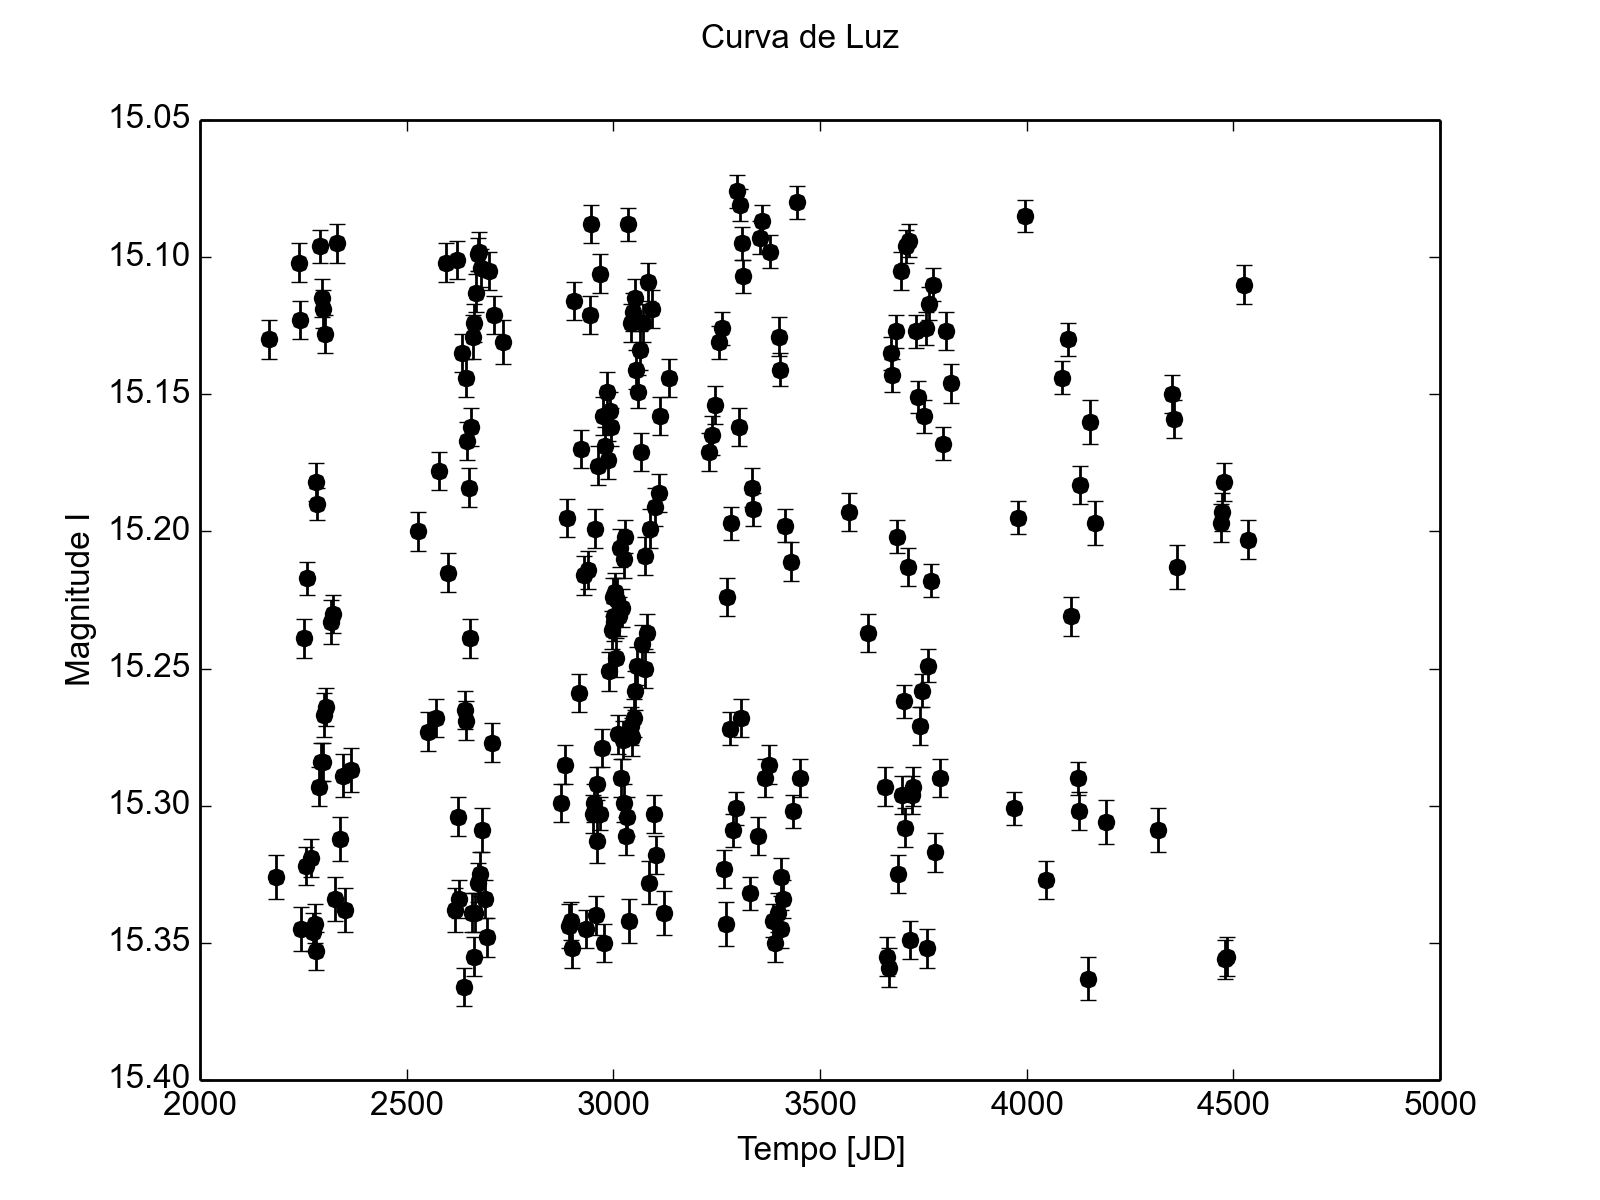
\includegraphics[width=0.7\linewidth]{0018_curva.png}
\caption[Exemplo de curva de luz]{Exemplo de curva de luz utilizando a Cefeida OGLE-LMC-CEP-0018 do catálogo OGLE. Podemos perceber o espaçamento entre os conjuntos de pontos.}
\label{fig:curva_luz}
\end{figure}


\subsection{Fase e o Espaço de Fase}

Quando uma estrela possui um comportamento periódico, a variação em sua magnitude é representada em ciclos iguais. Cada ciclo é uma fase. Se os ciclos são iguais, não importa qual ciclo nós estamos observando, apenas onde nós estamos no ciclo. Com isso, o espaço de fase é uma representação de todos os ciclos observados em apenas uma fase, ou em apenas um ciclo. Desta forma, os pontos se sobrepõem e formam uma oscilação geral da estrela. A fase é calculada pela seguinte expressão,
\begin{equation}
\phi_i = \frac{t_i}{P} - \Big[\frac{t_i}{P}\Big]
\end{equation}
em que $t_i$ é o i-ésimo dado do tempo, $P$ é o período de oscilação da magnitude e a quantidade entre colchetes representa apenas o numero inteiro da divisão. O espaço de fase é o gráfico da magnitude aparente versus a fase.


\begin{figure}[!ht]
\centering
\begin{subfigure}{.5\textwidth}
  \centering
  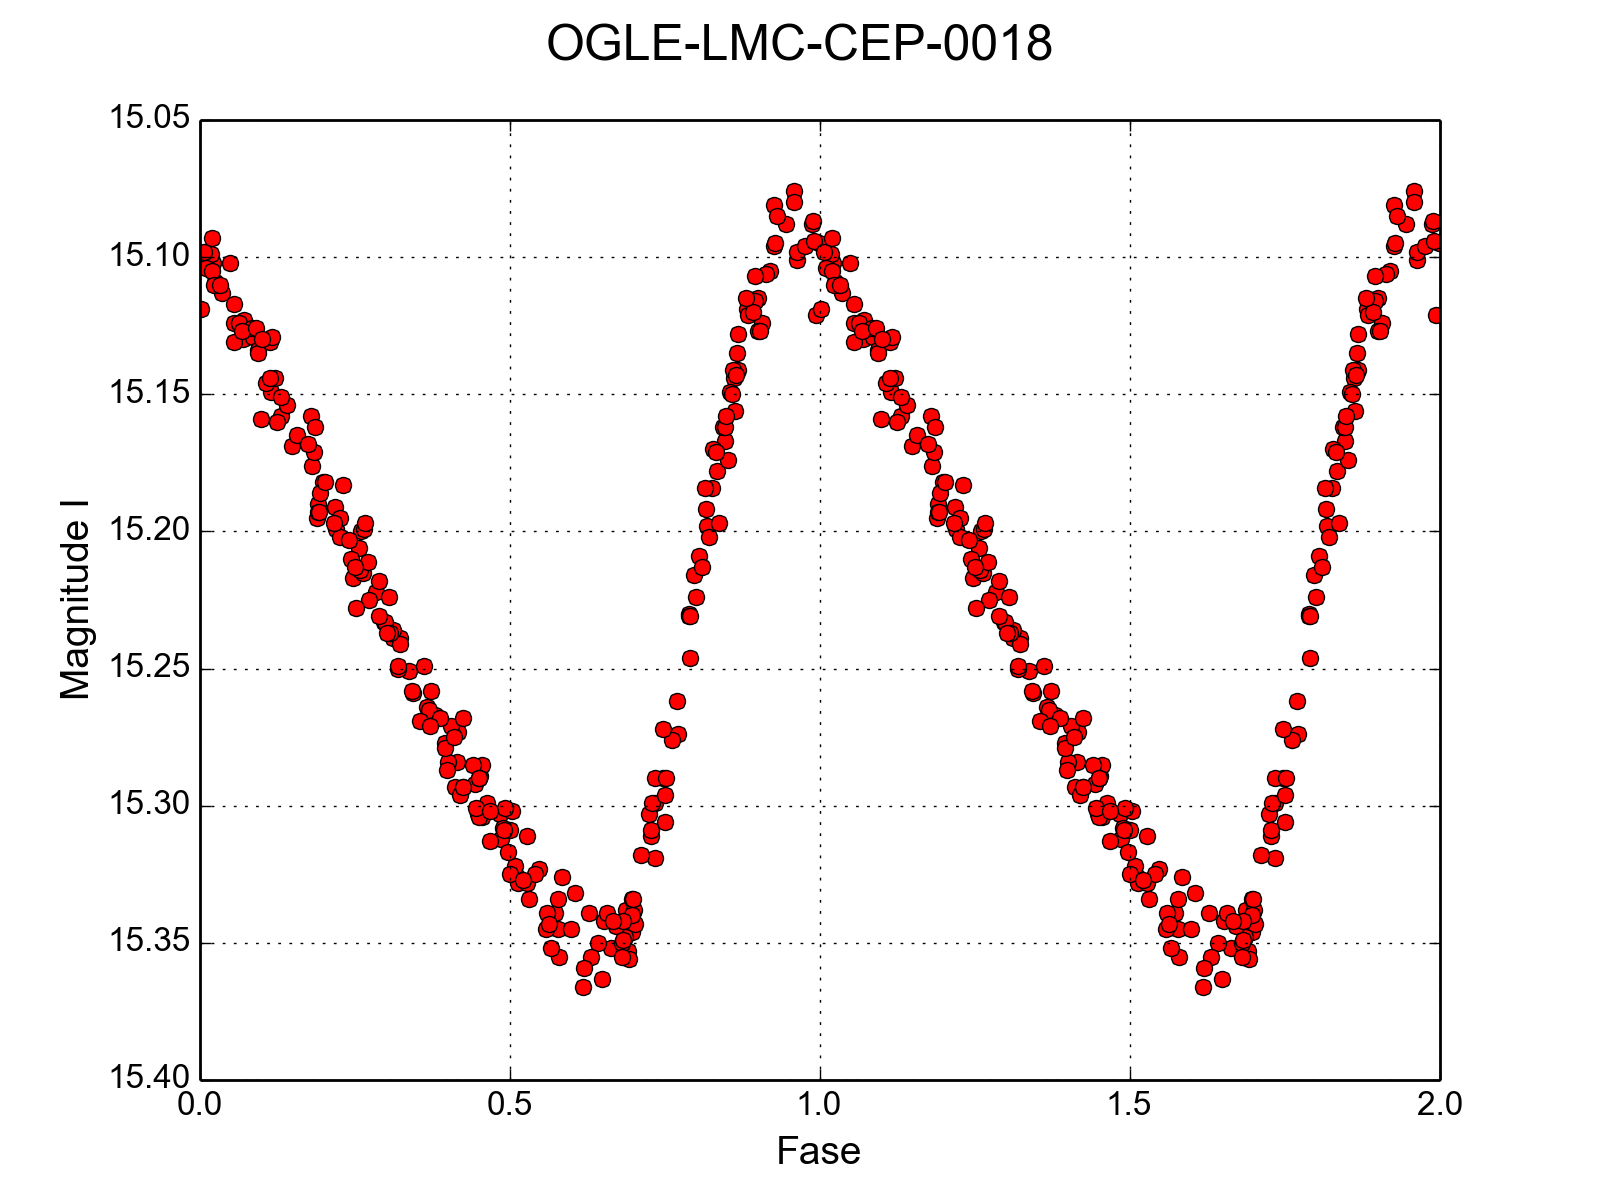
\includegraphics[width=\linewidth]{0018_correct.png}
  \caption{Período correto}
  \label{fig:right}
\end{subfigure}%
\begin{subfigure}{.5\textwidth}
  \centering
  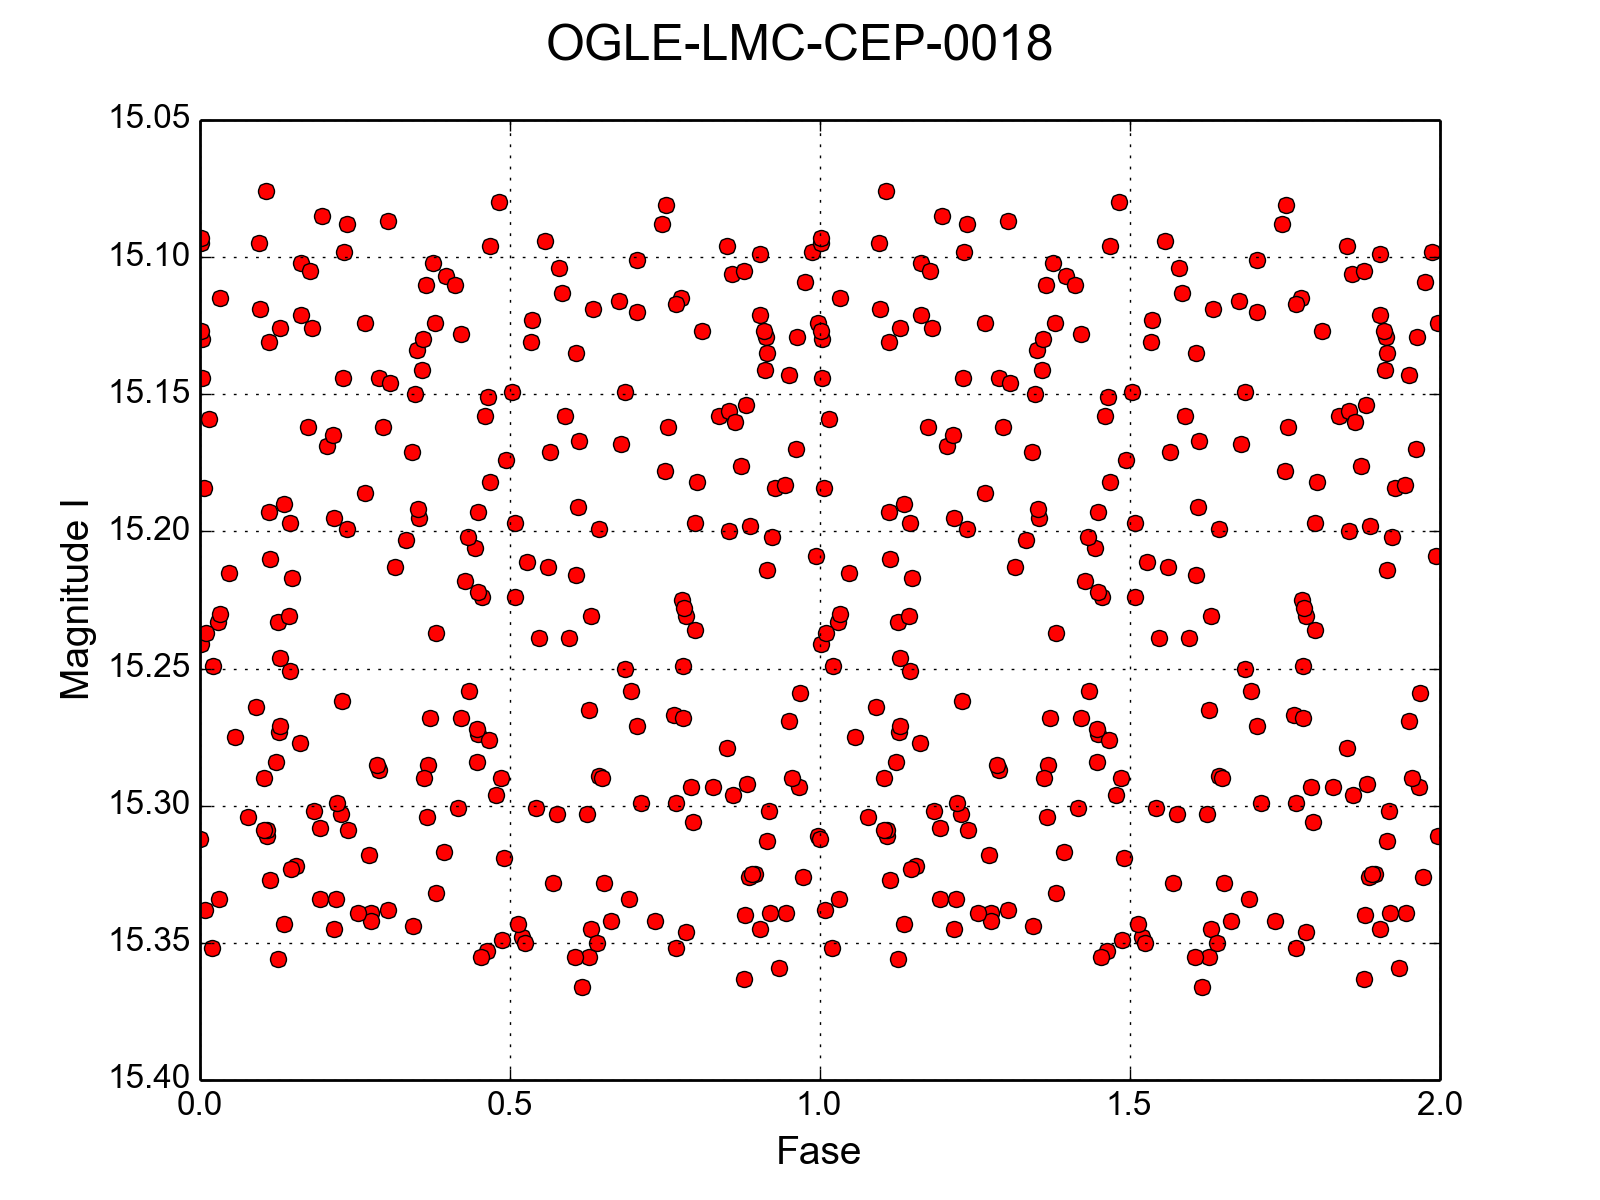
\includegraphics[width=\linewidth]{0018_wrong.png}
  \caption{Período errado}
  \label{fig:wrong}
\end{subfigure}
\caption[Exemplos de espaço de fase]{Exemplos de espaço de fase para a Cefeida OGLE-LMC-CEP-0018 do catálogo OGLE. O espaço de fase da imagem na esquerda foi construído utilizando o período correto da estrela ($P=4,0478$) e na imagem da direita foi utilizado um período aleatório ($P=3,0123$).}
\label{fig:exemplo_fase}
\end{figure}

Quando a série temporal de uma estrela periódica é dividida pelo período correto, será gerado uma dispersão com característica oscilante, como é o caso da figura \ref{fig:right}. Se o período utilizado na transformação não for o correto, será gerado uma dispersão aleatória, sem forma definida, como mostra a figura \ref{fig:wrong}.

%\subsection{Frequência de Nyquist}

%\subsection{Pulsação Estelar}
\subsection{Classificação Espectral}

A classificação espectral é uma forma de dividir as estrelas em relação aos elementos observados em seu espectro e em relação a sua temperatura. Esse método de classificação foi desenvolvido no laboratório de Harvard, nos Estados Unidos, no início do século XX %. A classificação foi desenvolvida
por Williamina Fleming (1857-1911), Antonia Caetana de Paiva Pereira Maury (1886-1952) e Annie Jump Cannon (1863-1941) que classificaram $225000$ estrelas até magnitude $9$.  A classificação espectral assim como a cor correspondente das estrelas, temperatura efetiva e as características das linhas espectrais podem ser vista na tabela \ref{tab:tipo_espectral}.

\begin{table}[!ht]
\begin{center}
\captionof{table}{Classificação Espectral.}
\begin{tabular}{c|c|c|c}
\toprule%\hline
Tipo Espectral & Cor & $T_{eff} \ \si{K}$ & Linhas no Espectro  \\
\midrule%\hline
O & Azul & 20000 a 40000 & HeII e HI \\
B & Branca-azulada & 15000 & HeI e HI\\
A & Branca & 9000 & HI \\
F & Branca-amarelada & 7000 & HI e CaII \\
G & Amarela & 5500 & HI e CaII\\
K & Laranja & 4000 & Linhas Metálicas \\
M & Vermelha & 3000 & CaI \\
\bottomrule%\hline
\end{tabular} \\
\small
\vspace{2mm}Fonte: Extraído de \citet{keplerLivro2013}.
\label{tab:tipo_espectral}
\end{center}
\end{table}


\subsection{Diagrama H-R}

O Diagrama H-R foi descoberto por Ejnar Hertzsprung (1873-1967) e Henry Russell (1877-1957) em 1913. Esse diagrama apresenta uma relação entre a luminosidade de uma estrela e a sua temperatura superficial. Hertzsprung descobriu que estrelas com uma mesma cor podiam ser divididas pela sua luminosidade, chamando as mais luminosas de gigantes e as menos luminosas de anãs.

\begin{figure}[!ht]
\centering
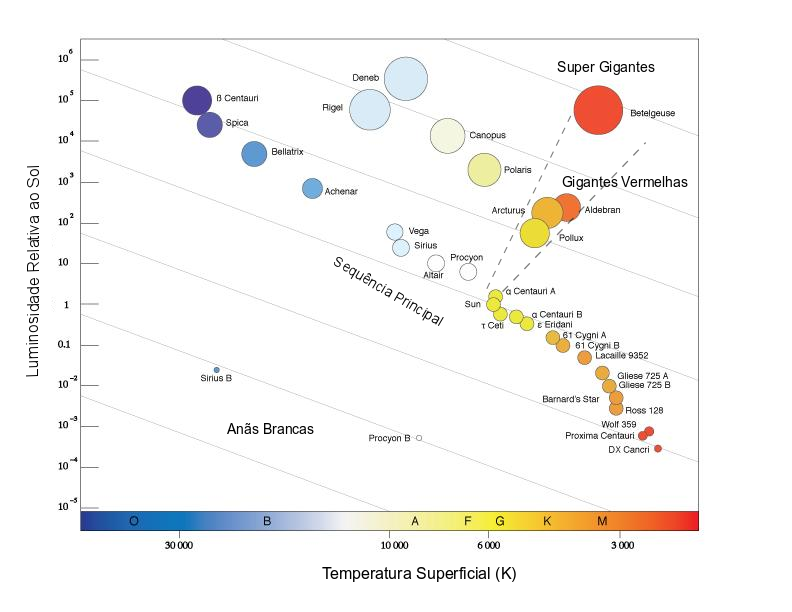
\includegraphics[width=\linewidth]{hr_diagrama.png}
\caption[Diagrama H-R.]{Diagrama H-R. O eixo das abcissas representa a temperatura superficial da estrela e por convenção cresce para à esquerda. Nesse mesmo eixo podemos ver a classificação espectral. O eixo das ordenadas representa a luminosidade das estrelas relativa com a luminosidade do Sol. As linhas diagonais no diagrama representam o tamanho do raio da estrela, quanto mais para o topo do diagrama, maior o raio. As linhas tracejadas delimitam a região chamada de faixa de instabilidade. Disponível em <\url{http://henrietta.iaa.es/el-harén-de-pickering-antonia-c-maury}>. Acessado e adaptado em maio de 2016.}
\label{fig:diagrama_hr}
\end{figure}

No diagrama H-R (figura \ref{fig:diagrama_hr}) o eixo das abcissas representa a temperatura que cresce para à esquerda e o eixo das ordenadas representa a luminosidade. Podemos dividir o diagrama em algumas seções. Uma dessas seções é a \textit{Sequência Principal}, que cobre a faixa na diagonal que vai do extremo direito inferior (estrelas frias e pouco luminosas) até o extremo esquerdo superior (estrelas quentes e muito luminosas). Na região superior direita acima da sequência principal há uma região chamada \textit{Gigantes Vermelhas} pois é onde esses tipos de estrelas se localizam. Essas estrelas são frias porém luminosas, o que indica um tamanho maior. Acima das Gigantes Vermelhas há a região das \textit{Supergigantes} que apresentam grande luminosidade. Por fim, no canto inferior esquerdo há a região das \textit{Anãs Brancas}, estrelas quentes e pouco luminosas, o que indica o seu tamanho reduzido.

Um fator que determina a posição de uma estrela no digrama H-R é a sua massa. Quanto mais massiva a estrela, mais quente e luminosa ela se torna. Também é possível interpretar o diagrama como uma relação entre massa e temperatura, pois a luminosidade é proporcional a massa da estrela.

Existe uma versão do diagrama H-R para estrelas variáveis. Nele é possível ver a localização de diversos tipos dessas estrelas. Essa versão do diagrama pode ser visto na figura \ref{fig:hr_variavel}. Nesse diagrama uma região importante é a chamada \textit{faixa de instabilidade} onde se localizam a maioria das estrelas variáveis pulsantes. Essa região é localizada entre as linhas tracejadas da figura \ref{fig:hr_variavel}.

\begin{figure}[ht!]
\centering
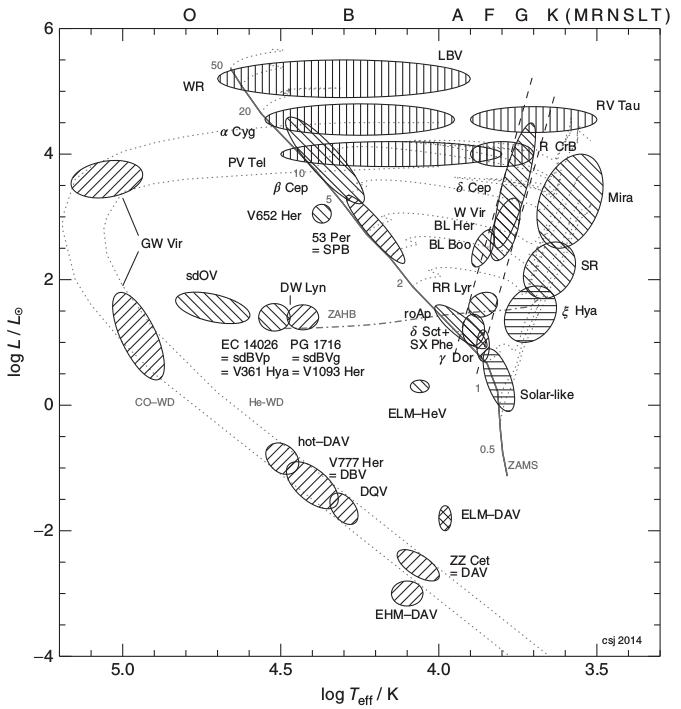
\includegraphics[width=\linewidth]{variability_hr_diagram.png}
\caption[Diagrama H-R para estrelas variáveis.]{Diagrama H-R para estrelas variáveis. A sequência principal é representada pela linha sólida. A região entre as linhas tracejadas representa a faixa de instabilidade onde estão localizadas diversas estrelas pulsantes. Adaptado de \citet{Catelan_book}.}
\label{fig:hr_variavel}
\end{figure}

\section{Pulsação Estelar}

%\nocite{astroseis}

Estrelas pulsam ou vibram de forma análoga a instrumentos de corda ou de sopro \citep{astroseis}. Cada instrumento possui uma frequência fundamental e o formato do objeto determina a sua frequência natural de vibração e seus harmônicos, que são múltiplos inteiros da frequência natural. A combinação destas frequências, amplitudes e fases dos harmônicos definem o timbre do instrumento, ou seja, o seu som característico. Logo, o formato interno do instrumento gera um som característico e, a partir das frequências emitidas podemos inferir o formato interno do instrumento.

De forma análoga, através da pulsação nós podemos determinar o formato interno da estrela. Porém, as estrelas não possuem harmônicos de vibração, elas possuem sobretons. Um sobretom é qualquer frequência acima da frequência natural de pulsação. Tecnicamente, os harmônicos são sobretons, mas nem todos sobretons são harmônicos. Dentro da astrofísica há um ramo chamado de astrossismologia que tem como objetivo medir a velocidade do som dentro das estrelas e determinar os parâmetros da estrutura interna destes corpos celestes. Portanto, a pulsação das camadas externas das estrelas nos dão informação a respeito dos processos que ocorrem no seu interior.

Porém, diferente de instrumentos onde há apenas ondas sonora se propagando, nas estrelas ocorrem os modos P (ondas sonoras) e modos G de pulsação. Estes modos também são chamados respectivamente de modos de pressão e modos de gravidade. Para entender melhor como ocorre a pulsação nas estrelas, vamos analisar alguns casos mais simples.

\subsection{Oscilação em uma corda}
No caso de oscilação mais simples, temos uma corda oscilando unidimensionalmente com as suas extremidades fixas. As frequências de oscilação dependem do comprimento $L$, da tensão $T$ e do material com o qual a corda é feita. Geralmente, a composição da corda e sua tensão são uniformes ao longo de seu comprimento. Assim, o primeiro harmônico (ou sobretom) é duas vezes a frequência fundamental ($2\omega_0$) o segundo harmônico é três vezes frequência fundamental ($3\omega_0$) e assim por diante, sendo o comprimento da corda relacionado com a frequência e comprimento de onda da seguinte forma \citep{astroseis}:
\begin{align}
\omega_0 = \frac{v}{2L} \quad \text{e} \quad L = \frac{\lambda}{2}
\end{align}
Em que $v$ é a velocidade da onda na corda e $\lambda$ o comprimento de onda. Um exemplo de pulsação em corda fixa pode ser visto na figura \ref{fig:corda}.

\begin{figure}[!ht]
\centering
\begin{subfigure}{.33\textwidth}
  \centering
  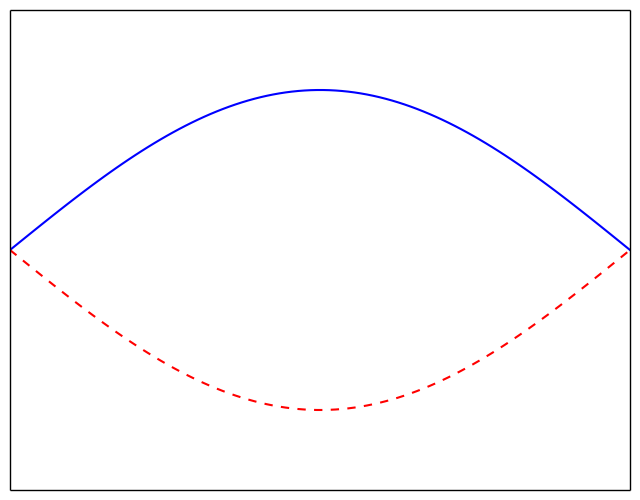
\includegraphics[width=\linewidth]{pulsacao_1d_corda_fu.png}
  \caption{Frequencia Fundamental}
  %\label{fig:right}
\end{subfigure}%
\begin{subfigure}{.33\textwidth}
  \centering
  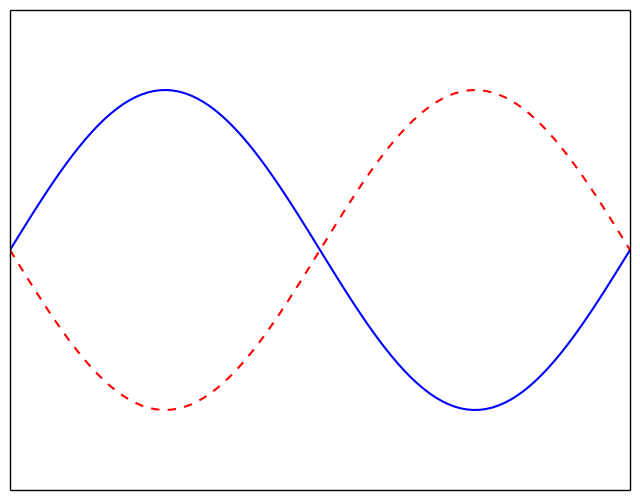
\includegraphics[width=\linewidth]{pulsacao_1d_corda_FO.png}
  \caption{Primeiro Harmônico}
  %\label{fig:wrong}
\end{subfigure}
\begin{subfigure}{.33\textwidth}
  \centering
  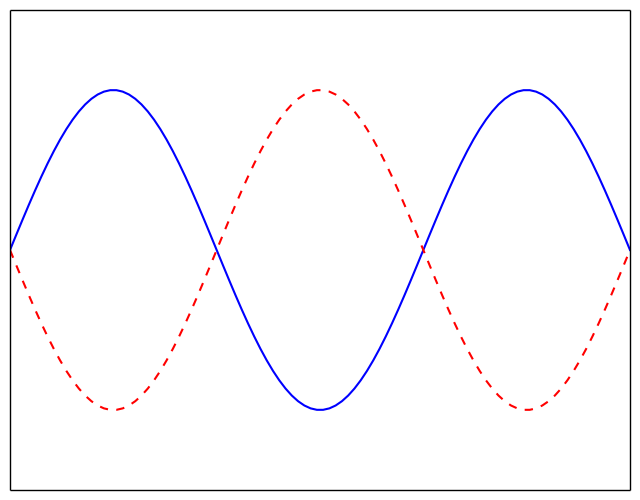
\includegraphics[width=\linewidth]{pulsacao_1d_corda_SO.png}
  \caption{Segundo Harmônico}
  %\label{fig:wrong}
\end{subfigure}
\caption[Oscilação em uma corda com extremidades fixas]{Exemplos de oscilação em uma corda com as extremidades fixas. A imagem da esquerda (a) representa a oscilação na frequência natural. A figura do meio (b) representa a pulsação no primeiro harmônico. Por ultimo, a imagem da direita (c) representa oscilação no segundo harmônico.}
\label{fig:corda}
\end{figure}

\subsection{Oscilação em uma corda com uma extremidade fixa}

Neste caso, temos uma corda que oscila de forma unidimensional e possui uma de suas extremidades fixa e a outra solta. Este exemplo é semelhante a um instrumento de sopro que possui uma extremidade fechada. A parte fixa da corda, ou fechada do instrumento de sopro, atua como um nó (ponto onde a amplitude é zero) e na extremidade fixa a amplitude é máxima (ou mínima). No caso do instrumento de sopro, como a temperatura e composição do gás são uniformes na parte interna do instrumento, a velocidade do som é constante nessa região. Para este caso, os harmônicos são múltiplos ímpares da frequência fundamental, por exemplo, $3\omega_0$, $5\omega_0$, etc.. A relação entre o comprimento da corda e a frequência fundamental assim como a relação com o comprimento de onda é dado por \citep{astroseis}:
\begin{align}
\omega_0 = \frac{v}{4L} \quad \text{e} \quad L = \frac{\lambda}{4}
\end{align}
Um exemplo deste comportamento pode ser visto na figura \ref{fig:corda_fixa}.

\begin{figure}[!ht]
\centering
\begin{subfigure}{.33\textwidth}
  \centering
  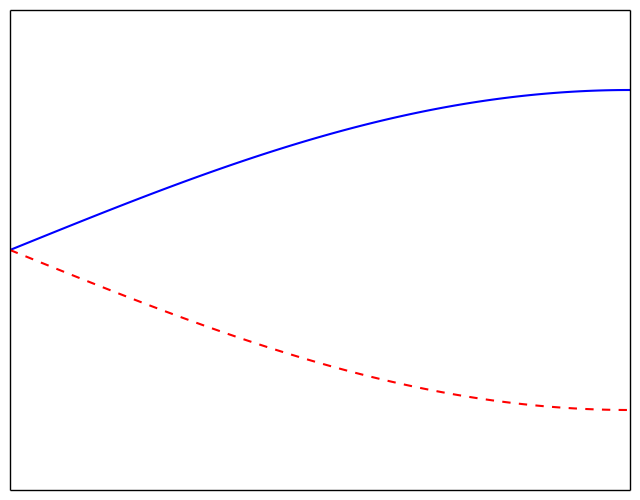
\includegraphics[width=\linewidth]{pulsacao_1d_sopro_FU.png}
  \caption{Frequência Fundamental}
  %\label{fig:right}
\end{subfigure}%
\begin{subfigure}{.33\textwidth}
  \centering
  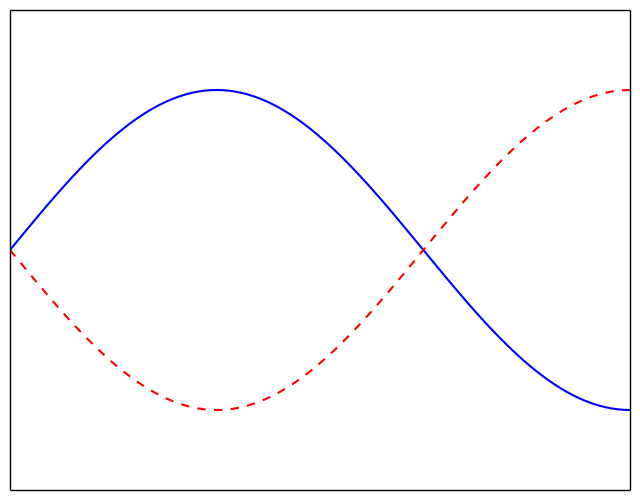
\includegraphics[width=\linewidth]{pulsacao_1d_sopro_FO.png}
  \caption{Primeiro Harmônico}
  %\label{fig:wrong}
\end{subfigure}
\begin{subfigure}{.33\textwidth}
  \centering
  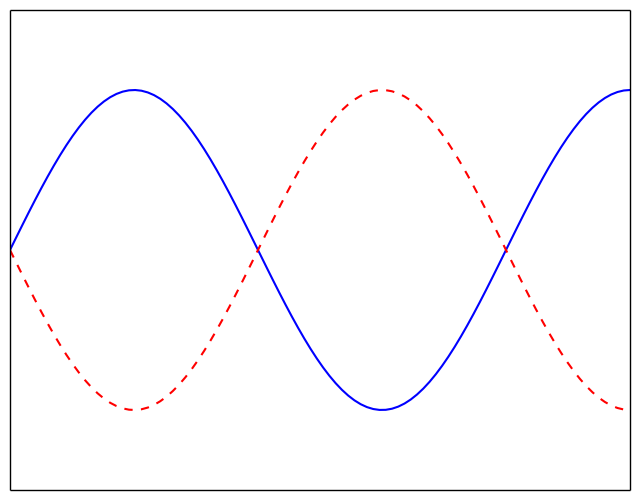
\includegraphics[width=\linewidth]{pulsacao_1d_sopro_SO.png}
  \caption{Segundo Harmônico}
  %\label{fig:wrong}
\end{subfigure}
\caption[Oscilação em uma corda.]{Exemplo de oscilação em uma corda com uma extremidade fixa e outra solta. A imagem (a) representa o modo fundamental, a imagem (b) representa o primeiro harmônico e a imagem (c) representa o segundo harmônico.}
\label{fig:corda_fixa}
\end{figure}

\subsection{Oscilação bidimensional}

Para o caso bidimensional vamos utilizar um disco como exemplo. Existem dois tipos de nós no caso bidimensional. Estes nós são ortogonais e podem ser classificados como radiais (modo radial) e não-radiais.

Os nós radiais são círculos concêntricos ao disco. A frequência fundamental de vibração para o modo radial é semelhante à frequência fundamental da corda com as extremidades fixas, o centro do disco terá amplitude máxima e mínima enquanto que a borda possui amplitude zero (nó). O primeiro sobretom radial possui um nó com formato de um circulo concêntrico onde o disco interno possui amplitude máxima e o disco externo amplitude mínima e vice e versa. O segundo sobretom radial possui dois nós, ou seja, dois círculos concêntrico e portanto há três áreas onde a amplitude varia de máxima a mínima \citep{astroseis}.

\begin{figure}[htb!]
\centering
\begin{subfigure}{.33\textwidth}
  \centering
  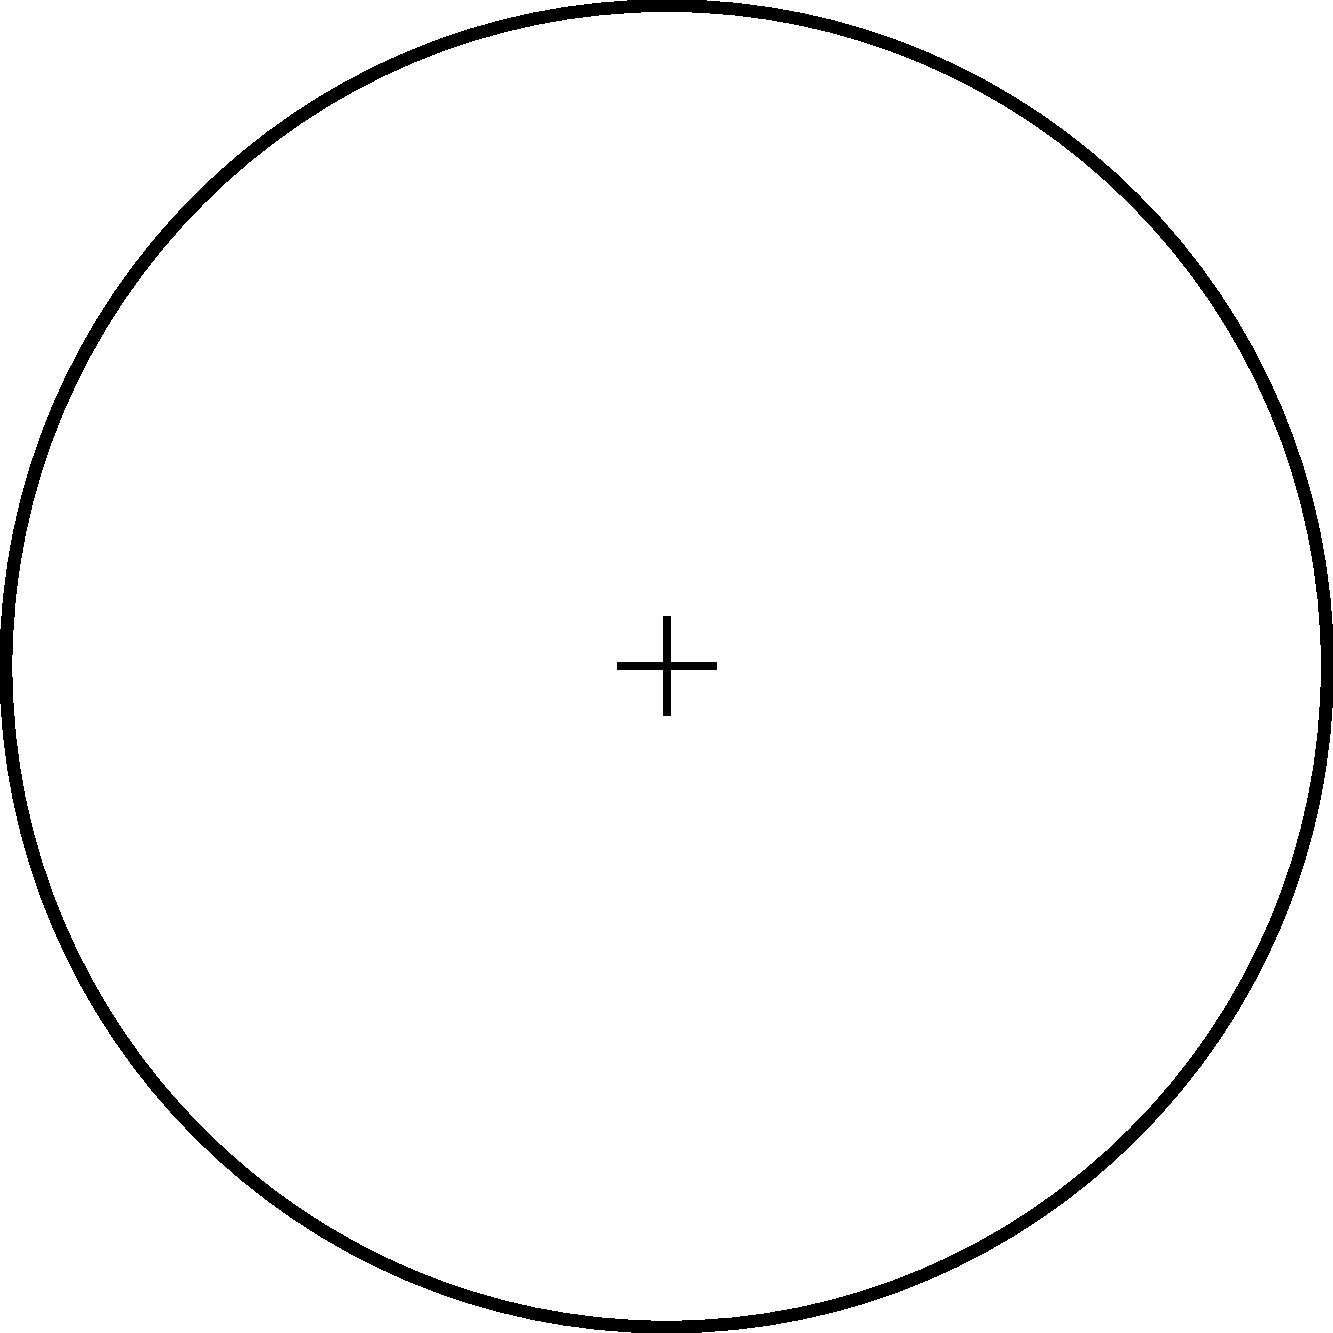
\includegraphics[width=\linewidth]{pulsacao_2d_radial_FU.pdf}
   \caption{Frequência Fundamental}
  %\label{fig:right}
\end{subfigure}%
\begin{subfigure}{.33\textwidth}
  \centering
  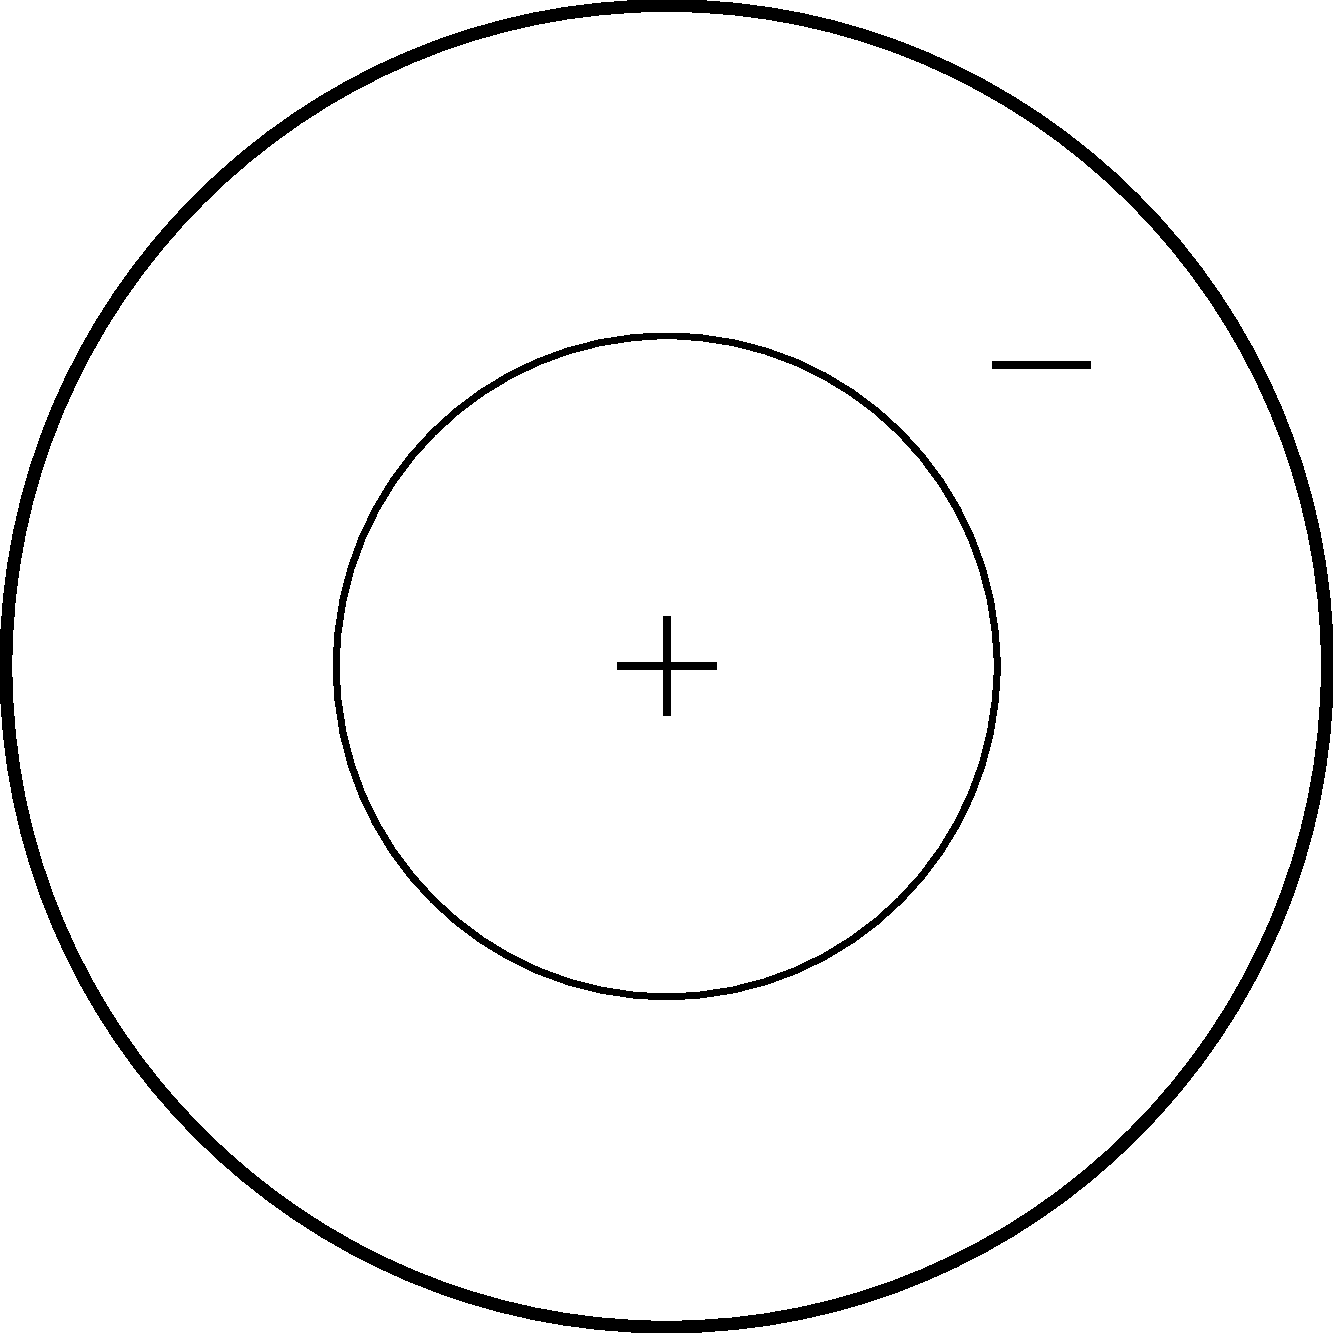
\includegraphics[width=\linewidth]{pulsacao_2d_radial_FO.pdf}
  \caption{Primeiro Sobretom}
  %\label{fig:wrong}
\end{subfigure}
\begin{subfigure}{.33\textwidth}
  \centering
  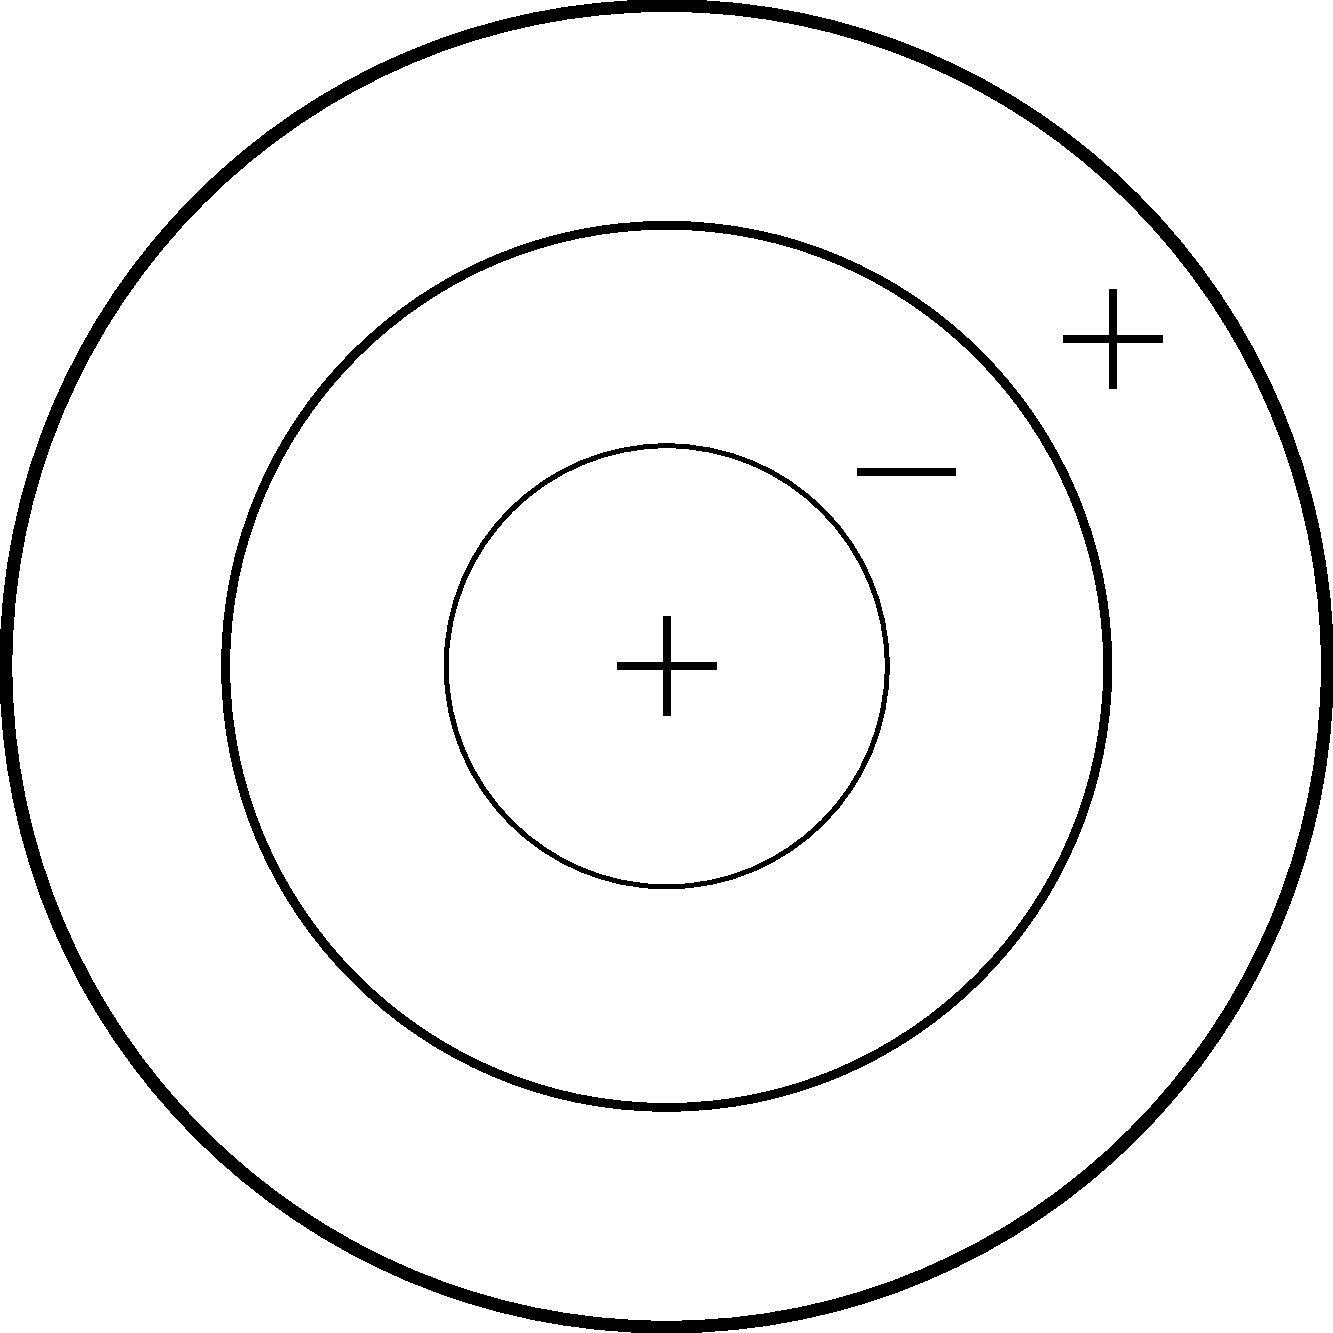
\includegraphics[width=\linewidth]{pulsacao_2d_radial_SO.pdf}
  \caption{Segundo Sobretom}
  %\label{fig:wrong}
\end{subfigure}
\caption[Oscilação radial em um disco.]{Exemplo de oscilação radial em um disco. Os sinais $+$ e $-$ significam os pontos de máximo e mínimo. A imagem (a) representa o a frequência fundamental, a imagem (b) representa o primeiro sobretom e a imagem (c) representa o segundo sobretom.}
\label{fig:disco_radial}
\end{figure}

A segunda forma de nós são os nós não-radiais. O primeiro nó não-radial é uma linha que divide o disco ao meio. Com isto, as duas metades do disco oscilam de forma oposta, enquanto uma possui o máximo de amplitude a outra metade possui o mínimo. O segundo nó não-radial são duas linhas ortogonais que dividem o disco em quatro partes com cada parte oscilando de forma contraria a outra.

\begin{figure}[htb!]
\centering
\begin{subfigure}{.33\textwidth}
  \centering
  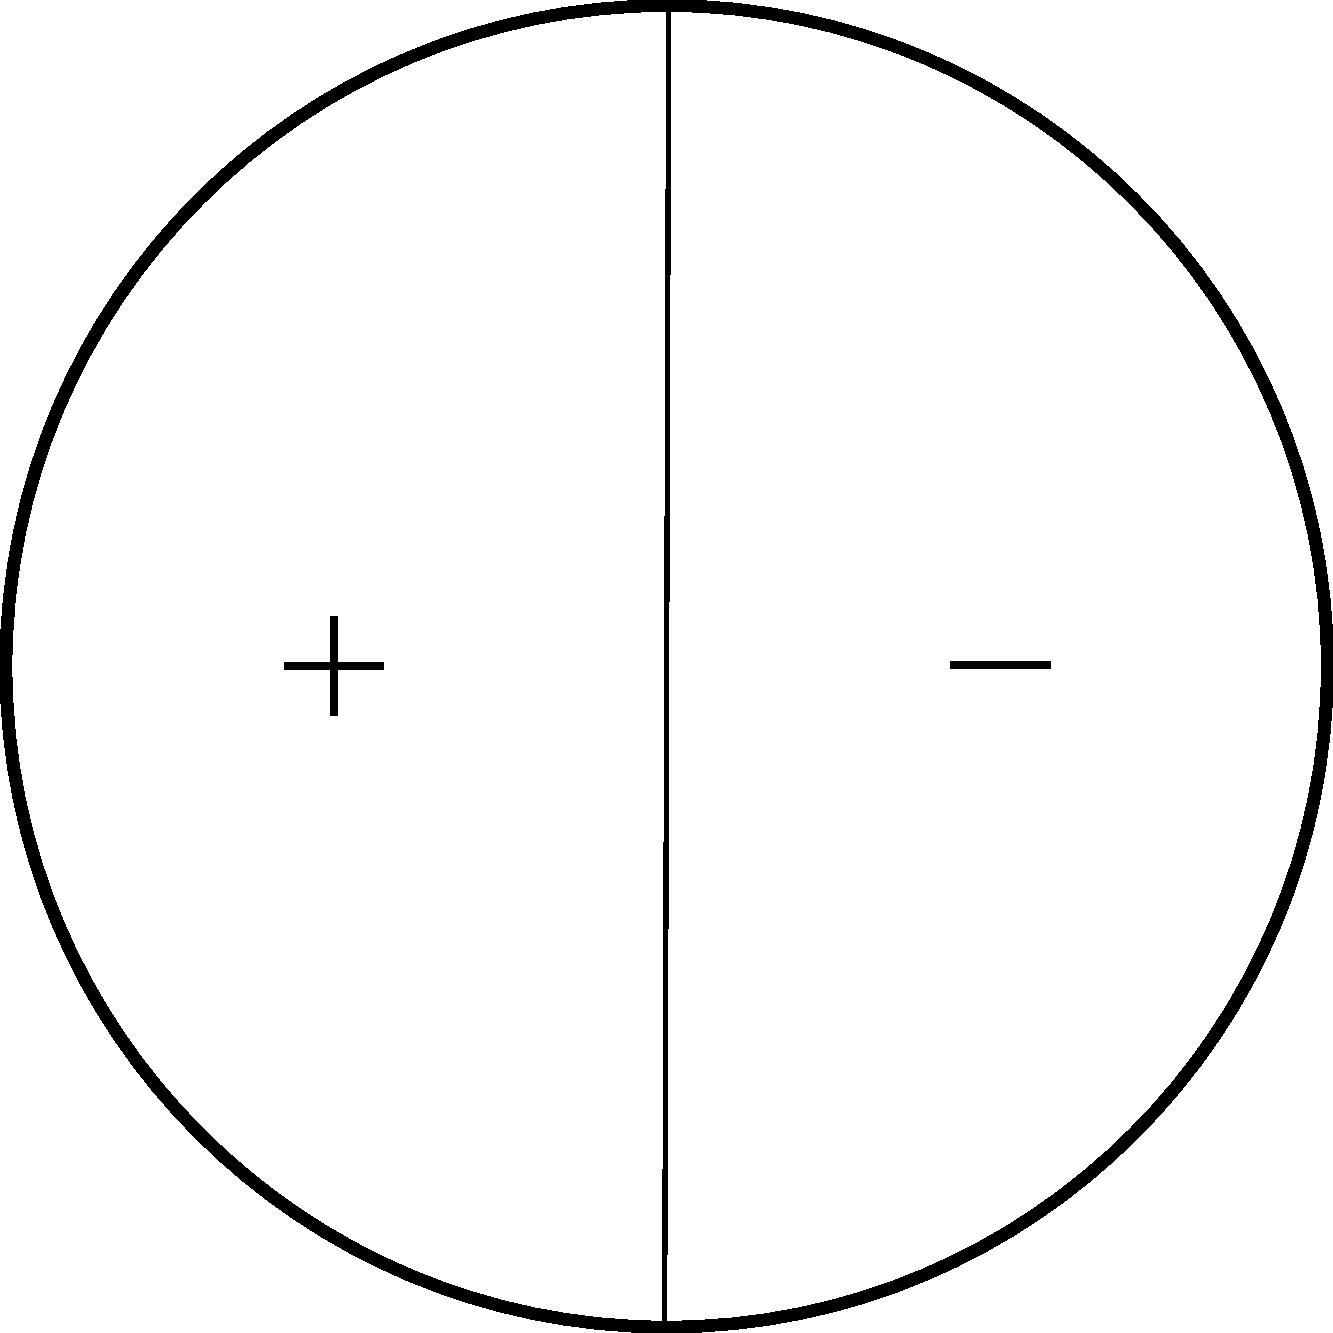
\includegraphics[width=\linewidth]{pulsacao_2d_naoradial_FU.pdf}
  \caption{Frequência Fundamental}
  %\label{fig:right}
\end{subfigure}%
\hspace{2mm}
\begin{subfigure}{.33\textwidth}
  \centering
  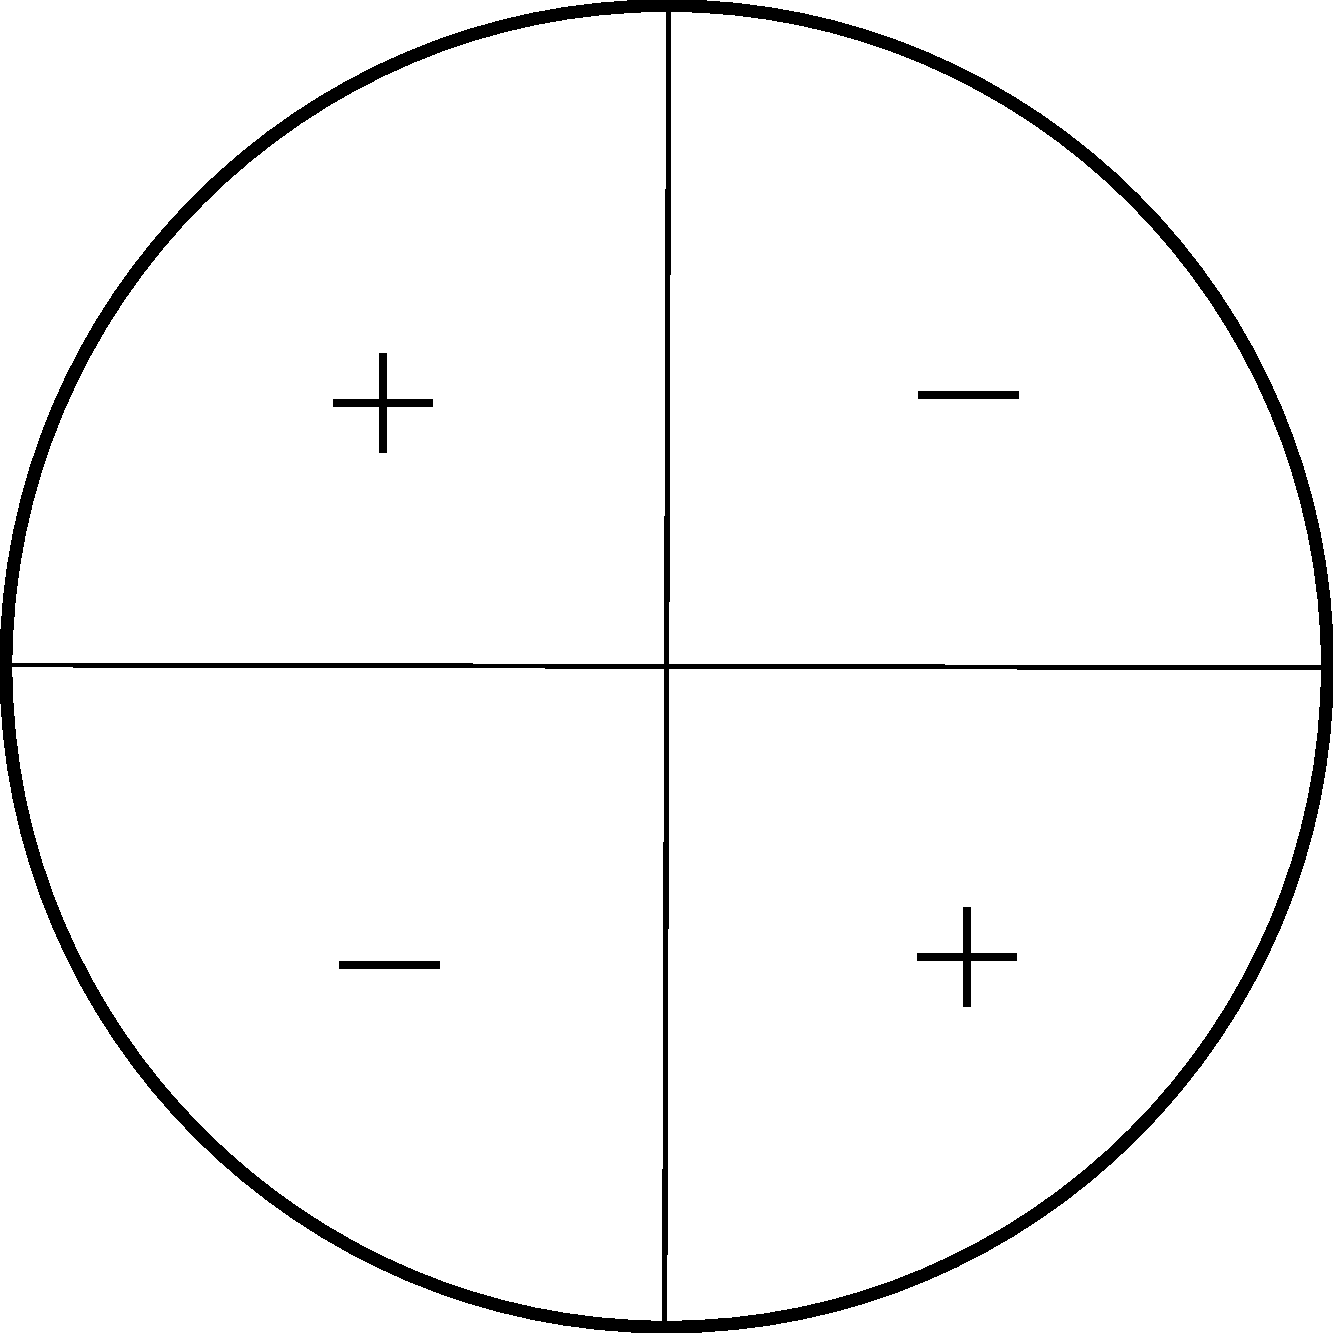
\includegraphics[width=\linewidth]{pulsacao_2d_naoradial_FO.pdf}
  \caption{Primeiro Sobretom}
  %\label{fig:wrong}
\end{subfigure}
\caption[Oscilação não-radial em um disco.]{Exemplo de oscilação não-radial em um disco. A imagem (a) representa a frequência fundamental e a imagem (b) representa o primeiro sobretom.}
\label{fig:disco_naoradial}
\end{figure}

Porém, essas duas formas de oscilação não ocorrem isoladamente pois, geralmente há combinações dos sobretons radiais e não radiais nas estrelas.
\begin{figure}[h]
\center
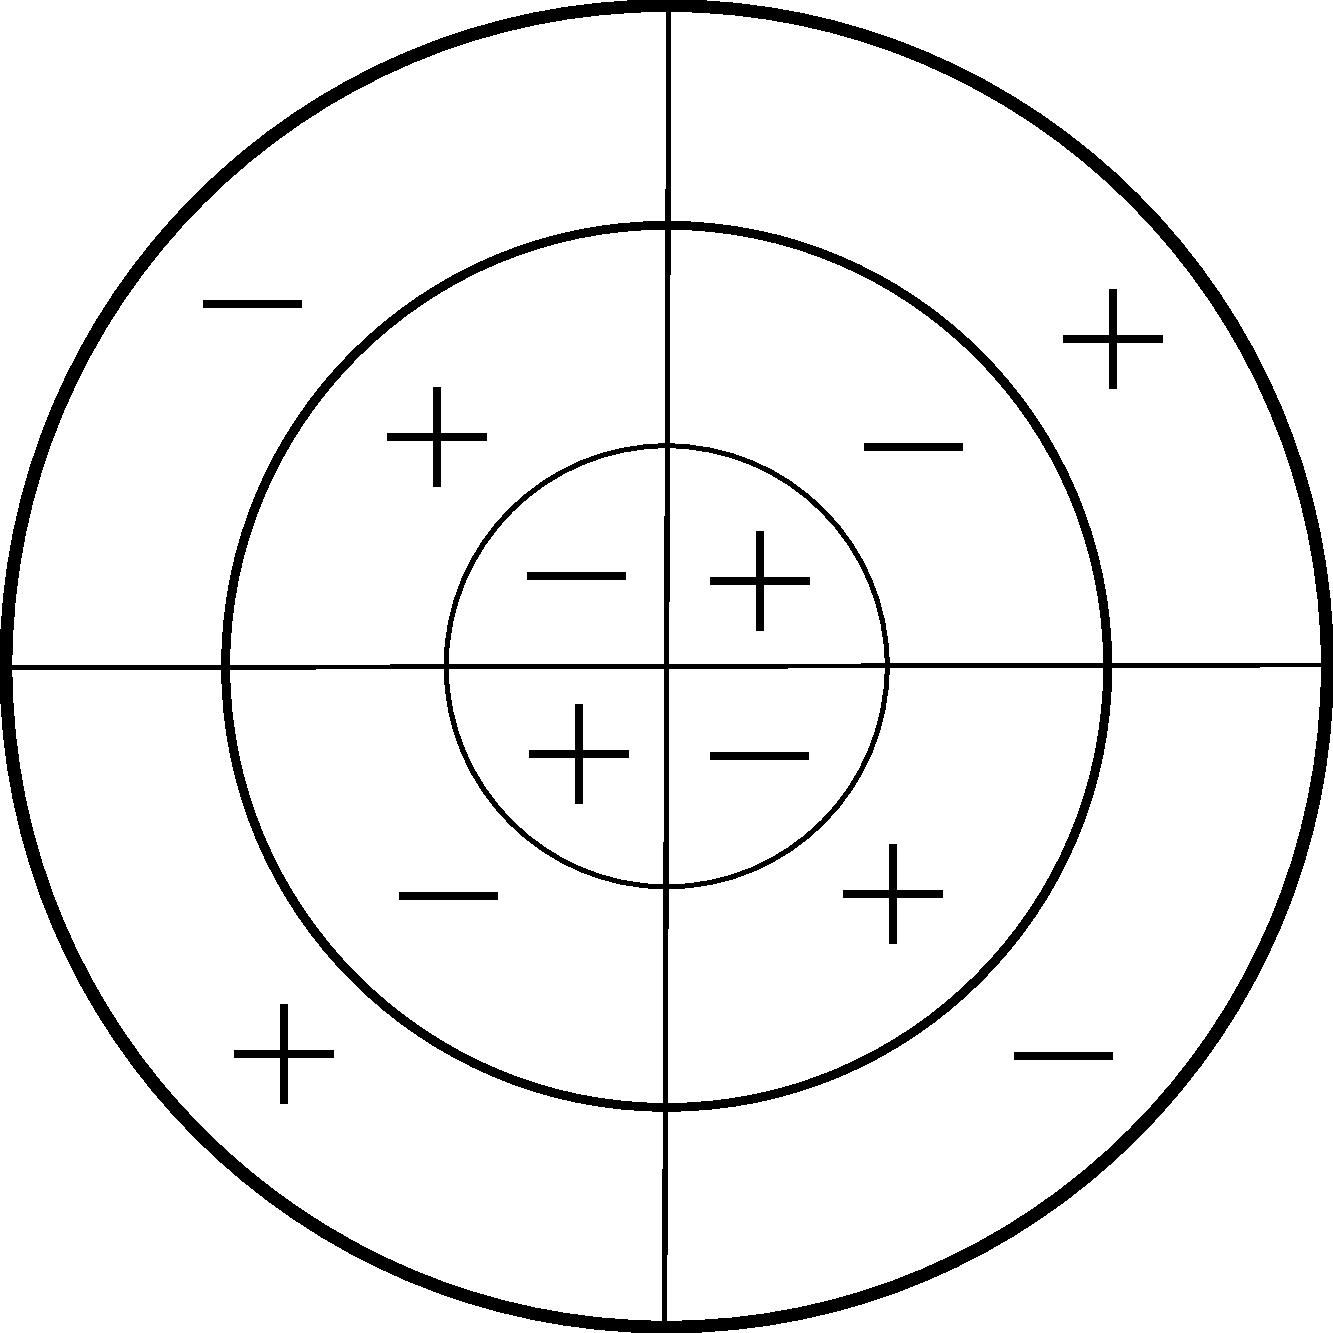
\includegraphics[width=0.33\linewidth]{pulsacao_2d_naoradial_SO.pdf}
\caption{Oscilação radial e não-radial em um disco.}
\end{figure}

\subsection{Oscilações em 3 dimensões}
%ler sobre eixo de rotacao e de pulsacao
Estrelas possuem um formato esférico e suas pulsações obedecem os modos de oscilações em 3 dimensões.
De forma análoga ao disco que possui dois modos de pulsação em direções ortogonais, as oscilações em uma esfera possuem três modos  em direções ortogonais. Estas direções são a distancia do centro $r$, latitude $\theta$ e longitude $\phi$. Os nós serão compostos por cascas esféricas de tamanho $r$, cones de tamanho $\theta$ e planos de dimensão $\phi$.

Para uma estrela simétrica, as soluções das equações de movimento ondulatório são as seguintes \citep{astroseis},
\begin{align}
\xi_{r}(r , \theta , \phi , t) &= a(r) \; Y_{l}^{m}(\theta , \phi) \; exp(-i2\pi\nu t) \\
\xi_{\theta}(r , \theta , \phi , t) &= b(r) \; \frac{\partial Y_{l}^{m}(\theta , \phi)}{\partial\theta} \; exp(-i2\pi\nu t) \\
\xi_{\phi}(r , \theta , \phi , t) &= \frac{b(r)}{\sin\theta} \; \frac{\partial Y_{l}^{m}(\theta , \phi)}{\partial\phi} \; exp(-i2\pi\nu t)
\end{align}
em que $a(r)$ e $ b(r)$ são amplitudes, $ \nu $ é a frequência de oscilação e $ Y^m_l(\theta , \phi) $ são esféricos harmônicos que são calculados da seguinte forma \citep{astroseis},
\begin{align}
Y^m_l(\theta , \phi) = (-1)^m \sqrt{\frac{2l+1}{4\pi}\frac{(l-m)!}{(l+m)!}} \; P_l^m(\cos\theta) \; exp(im\phi)
\end{align}
onde $ P_l^m(\cos\theta)$ são polinômios de Legendre dados por \citep{astroseis},
\begin{align}
P_l^m(\cos\theta) = \frac{1}{2^l l!}(1-\cos^2\theta)^{m/2}\frac{d^{l+m}}{d\cos^{l+m}\theta}(\cos^2\theta - 1)^l .
\end{align}
As letras $ l$ e $ m $ são o grau da função harmônica e a ordem, que são números inteiros e caracterizam os modos de pulsação. A variação destes números indicam se haverá pulsação radial ou não-radial.

\subsubsection{Modo radial}

Na pulsação radial o número $ l$ é igual a zero. O modo mais simples de pulsação radial é chamado de modo fundamental radial. Neste modo, a estrela se contrai e expande isotropicamente de forma simétrica. Este é o principal modo de pulsação de estrelas Cefeidas e RR Lyrae.

O primeiro sobretom do modo radial possui um nó no interior da estrela. Este nó é uma casca esférica onde a amplitude é sempre zero. As camadas da estrela antes e depois deste modo se movem de forma oposta, ou seja, enquanto uma contrai a outra expande.

%$$ \text{exemplo de modo radial} $$

%Existem estrelas que pulsam com o modo fundamental e o primeiro sobretom ao mesmo tempo. Estas estrelas são classificadas como Cefeidas de modo duplo e RRLyraes tipo D.



\begin{figure}[!ht]
\centering
\begin{subfigure}{.5\textwidth}
  \centering
  
\includegraphics[scale=0.6]{3d_l3m0.png}
  \caption{$m = 0$}

\end{subfigure}%
\begin{subfigure}{.5\textwidth}
  \centering
  
\includegraphics[scale=0.6]{3d_l3m1.png}
  \caption{$m = \pm 1$}
\end{subfigure}
\\
\begin{subfigure}{.5\textwidth}
  \centering
  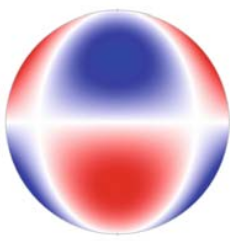
\includegraphics[scale=0.6]{3d_l3m2.png}
  \caption{$m = \pm 2$}

\end{subfigure}%
\begin{subfigure}{.5\textwidth}
  \centering
  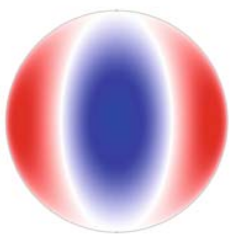
\includegraphics[scale=0.6]{3d_l3m3.png}
  \caption{$m = \pm 3$}
\end{subfigure}
\caption[Oscilação não-radial em uma esfera.]{Oscilação não-radial em uma esfera com $l=3$ e $ m$ variando de $0$ a $2$. As figuras mostram uma estrela vista de lado, com os polos sendo no topo e na região mais baixa. O equador seria exatamente no meio das esferas. As linhas brancas são os nós e a regiões em azul e vermelho estão contraindo e expandindo. Adaptado de \citet{astroseis}}
\label{fig:esfera_naoradial}
\end{figure}


\subsubsection{Modos não-radiais}

O modelo mais simples de pulsação não-radial possui $l=1$ e $ m=0 $. Neste modo, o equador da estrela é um nó, então um hemisfério expande enquanto o outro contrai. Este modelo também é chamado de modo de dipolo. O modo de pulsação com $ l=2$ possui dois nós na sua superfície e é chamado de modo de quadrupolo. Neste modo, os polos se expandem enquanto o equador contrai e vice e versa.
Na figura \ref{fig:esfera_naoradial} temos a representação de um modo de pulsação com $l=3$ e $m$ variando de $0$ a $2$.






%\subsection{Relação período-luminosidade}

%\subsection{Ascensão reta ($\alpha$)}

%\subsection{Declinação ($\delta$)}

%\section{Introdução Histórica - Estrelas Variáveis}
%\section{Introdução Histórica}

\section{Introdução Histórica às Estrelas Variáveis}

%\subsection{Estrelas Variáveis}
No século 16, acreditava-se que as estrelas eram fixas em posição e com brilho constante. Em 1572, foi observada uma supernova na constelação de Cassiopeia que atingiu magnitude $-4$. Este evento, que foi estudado por Tycho Brahe (1546-1601), fez com que a comunidade astronômica da época voltasse a se interessar pela descobertas de novas estrelas. Alguns anos mais tarde, em 1596, o holandês David Fabricius (1564-1617) fez o primeiro registro de variação em brilho de uma estrela na constelação da Baleia (Cetus).  Essa estrela foi observada em agosto e em outubro havia desaparecido. Em 1603, Johann Bayer observou a mesma estrela e deu o nome de omicron ($O$) Ceti, porém não sabia que era a mesma estrela que Fabricius havia observado, pois achava que se tratava de uma supernova. Em 1638, Johannes Holwarda (1618-1651) observou novamente $O$ Ceti. Em 1662, Johannes Hevelius (1611-1687) fez um estudo detalhado da estrela e a renomeou, chamando-a de Mira Ceti (a Maravilhosa). Ismael Bullialdus (1605-1694) percebeu que o pico de magnitude da estrela ocorria sempre um mês mais cedo a cada ano, descobrindo a natureza cíclica de sua variação de brilho. Bullialdus publicou em 1967 que o período de oscilação era de 333 dias. Essa estrela foi a primeira variável a ter o período conhecido e virou referência para as estrelas variáveis de períodos longos, conhecidas hoje em dia como as \textit{variáveis Mira}.

Em 1784, o inglês Jonh Goodricke (1764-1786) descobriu a variação no brilho da estrela $\delta$ Cephei. Ele mediu o período $5\si{\day}8\si{\hour}$. No mesmo ano, o inglês Edward Pigott (1753-1825) descobriu a variabilidade de $\eta$ Aquilae. Ambas estrelas se tornaram os protótipos da classe de \textit{variáveis Cefeidas}.

Em 1912, a americana Henrietta Swan Leavitt (1868-1921) derivou uma relação entre o período e a luminosidade (também conhecida como lei de Leavitt) para as estrelas Cefeidas localizadas na Pequena Nuvem de Magalhães \citep{Leavitt1912}. Graças a essa relação que em 1913 Hertzsprung foi capaz de calcular a primeira determinação de distância da Pequena Nuvem \citep{Hertzsprung1913}. Utilizando a mesma relação, Hubble determinou a distância de Andrômeda em 1923.


%\section{Introdução Histórica - Técnicas de Observação}
\subsection{Técnicas de Observação}

O primeiro dispositivo utilizado na observação de estrelas variáveis foi o olho humano.
Embora este dispositivo nos seja muito útil no dia-a-dia, para a observações de estrelas não seria o mais adequado, pois a sua precisão para captar brilho é baixa ($\approx 0.1$ magnitudes), o que faz com que apenas estrelas com variação de algumas unidades de magnitude nos chamaria a atenção. Da mesma forma, a percepção de mudanças no céu noturno não é possível com observações feitas em telescópios. Apenas com a introdução da placas fotográficas é que foi possível ter um controle mais efetivo desta variações.

%\subsection{Métodos fotográficos}
\subsubsection{Métodos fotográficos}

As primeiras fotografias astronômicas foram obtidas em torno de 1850 e 1860 utilizando o Daguerreótipo (ou método de Daguerre), que consistia em fixar a imagem em uma placa de cobre com uma fina camada de prata. Devido a sua limitação para variações em luminosidade, apenas fotos da Lua, Sol e estrelas mais brilhantes foram obtidas por este método. Apenas com o advento do método de placa seca em 1871 foi possível melhorar as observações de estrelas variáveis. Porém, identificar estrelas variáveis em placas fotográficas era um trabalho tedioso. Uma única imagem do céu noturno poderia conter milhares de estrelas. Uma forma utilizada para tentar identificar as variações de brilho seria utilizar uma série de 10 ou mais fotografias da mesma porção do céu, fazer divisões nas fotografias e comparar todas elas para perceber variações nos brilhos das estrelas. Através desta técnica aplicada em aglomerados globulares, o astrônomo Solon Bailey detectou mais de 500 variáveis \citep{Bailey1902}.

Outros métodos surgiram para aprimorar a identificação da estrelas variáveis. Um desses métodos seria a sobreposição dos negativos e positivos da mesma fotografia. No positivo, as estrelas seriam brancas em um fundo escuro enquanto que no negativo seria o oposto. Se o brilho de uma estrela variasse, a imagem negativa seria menor ou maior do que a imagem positiva.

Uma das principais ferramentas utilizadas para analisar as fotografias de estrelas era o dispositivo chamado \textit{Comparador Blink} (do inglês, \textit{Blink Comparator}). Nesse dispositivo, duas placas fotográficas eram analisadas, uma por cada olho do observador. Se as imagens fossem iguais, não seria identificado variação, porém alguma variação no brilho de uma imagem para a outra seria percebida pela mudança de tamanho da estrela entre as imagens.

Embora a quantidade de estrelas variáveis descobertas a partir de 1880 aumentou drasticamente devido aos métodos fotográficos, essa técnica não consegue identificar pequenas variações no brilho, apenas variações em torno de um terço da magnitude máxima da estrela, fazendo com que uma parcela das estrelas não fossem identificadas. Assim, surgiu a necessidade de algum método mais efetivo.


%\subsection{Métodos fotoelétricos}
\subsubsection{Métodos fotoelétricos}
O desenvolvimento da fotometria fotoelétrica ocorreu na década de 40. Esses métodos captam a luz em uma célula fotossensível que converte o fluxo de fótons recebido em sinal elétrico através do efeito fotoelétrico. Os sistemas de magnitudes (filtros) foram desenvolvidos para estes tipos de equipamentos.

Os primeiros dispositivos  desta época utilizavam placas de selênio e eram capazes de captar o brilho de apenas um objeto por vez. A magnitude de uma estrela era obtido fazendo a leitura do brilho da estrela e do céu noturno a sua volta, após era feita a leitura apenas de uma porção do céu e subtraído da leitura da estrela.

Uma das revoluções nesta área de observação ocorreu com a utilização das células fotomultiplicadoras na astronomia em 1936 pela Radio Corporation of America (RCA) \citep{Miles2007}. As vantagens dessas células são a amplificação do sinal observado, o que melhorou a precisão das medidas, maior faixa de detecção ($640 \si{nm}$ até a faixa do vermelho) e menor ruído. Embora a célula fotomultiplicadora tenha trazido grandes avanços na astronomia observacional, essa tecnologia ainda era limitada a observar objetos individuais. A grande revolução ocorreu com a utilização dos detectores em área.

%\subsection{Detectores em área}
\subsubsection{Detectores em área}

Em 1969 as placas CCD (do inglês, \textit{Charged Coupled Device}) foram criadas no Bell Laboratories nos Estado Unidos. Esse dispositivo apresenta alta sensibilidade espectral, podendo ser utilizado em faixas de $350$ a $1000 \si{nm}$. Também, possui a habilidade de detectar luz em área quando dispostas em conjunto (chamado de \textit{CCD Array}) e habilidade de transformar a observação em sinal digital sendo possível analisar as imagens em computadores, facilitando o trabalho de detecção de periodicidades através dos métodos de detecção de períodos.

%Atualmente, as placas CCD são os dispositivos utilizados no grandes projetos de levantamento de dados astronômicos (\textit{Surveys}). Um destes projetos é o OGLE que atualmente está atuando em sua quarta fase. A terceira fase \citep{Udalski2008} que já esta completa e possui seus dados públicos e utilizados nesse trabalho, monitorou mais de 200 milhões de estrelas nas Nuvens de Magalhães e se espera detectar em torno de um milhão de estrelas variáveis .


\section{Detecção de Períodos}

A busca por periodicidades na curva de luz de uma estrela variável é um dos mais importantes processos na análise de dados observacionais. A importância desse processo é devido as grandezas físicas que podemos derivar a partir do período. Dentro dessas grandezas, a distância é sem duvidas uma das mais importantes, pois a determinação de distâncias astronômicas é um dos problemas fundamentais da astronomia.

Devido a importância na determinação de períodos, diversos métodos surgiram ao longo dos anos. Uma técnica comum para demonstrar os períodos de uma estrela seria o \textit{Periodograma} ou \textit{Espectro de Potência}. Neste método, a intensidade do sinal gerado através dos dados é mostrado em um gráfico versus o período. Os picos desse gráfico seriam o período principal com os seu harmônicos. Alguns desse métodos utilizam o método dos mínimos quadrados para ajustar uma função com período conhecido à curva de luz da estrela \citep{lomb}. Outros determinam o período através dos picos no espectro de Fourier \citep{mello81} ou fazem analise de variância nesses picos \citep{aov}. Ou também, calculam a minimização da dispersão dos pontos observacionais no espaço de fase \citep{Cincotta1999, entropy, ce}.

Um dos principais problemas na determinação de períodos está nos dados observacionais. Dados que contenham uma semana de observação são impróprios para objetos que possuem período na ordem de anos. Para calcularmos o período com confiança, precisamos que o tempo de observação seja de pelo menos o dobro do tempo do período, de acordo com o \textit{Teorema de Nyquist} \citep{Nyquist1928}. Se esta condição não é satisfeita, podemos obter mais de um período ou o período errado para o nosso dado (este efeito é conhecido como \textit{Aliasing}). Outro motivo de erro nos dados são os espaçamentos entre as observações. Devido a estes espaçamento, as técnicas de detecção de períodos podem identificar períodos que aparentemente produzem uma curva de luz adequada, mas que não são os períodos corretos, sendo uma fonte de Aliasing. Alguns motivos para espaçamento entre os dados são a disponibilidade do telescópio, a limitação de observação para o turno da noite e a posição da lua nos telescópios terrestres, o que pode fazer com que as observações sejam espaçadas por até um mês. Por esses motivos apresentados, seria interessante aprimorar técnicas que sejam independentes deste espaçamento entre os dados, como as técnicas que utilizam a dispersão da curva de luz no espaço de fase, técnica utilizado pelo método aplicado neste trabalho.

\chapter{Justificativa e Objetivos}

por quê???
%!TEX root = /home/glauffer/Dropbox/FURG/final_project/monografia/monografia.tex
\chapter{Metodologia}
\label{cap:tecnicas}
%\textcolor{red}{descrição das técnicas em detalhes}

Neste capítulo será abordado o método utilizado para a determinação de períodos de estrelas variáveis pulsantes, assim como a metodologia aplicada para a análise do método e criação do algoritmo, cobrindo o catálogo utilizado para obtenção dos dados e o formato dos mesmos.

%A busca por periodicidades na curva de luz de uma estrela variável é um dos mais importantes processos na análise de dados observacionais. A importância desse processo é devido as grandezas físicas que podemos derivar a partir do período. Dentro dessas grandezas, a distância é sem duvidas uma das mais importantes pois, a determinação de distâncias astronômicas é um dos problemas fundamentais da astronomia.

%Devido a importância na determinação de períodos, diversos métodos surgiram ao longo dos anos. Uma técnica comum para demonstrar os períodos em um dado seria o \textit{Periodograma} ou \textit{Espectro de Potência}. Neste método, a intensidade do sinal gerado através dos dados é mostrado em um gráfico versus o período. Os picos desse gráfico seriam o período principal com os seu harmônicos. Alguns desse métodos utilizam o método dos mínimos quadrados para ajustar uma função com período conhecido à curva de luz da estrela \citep{lomb}. Outros determinam o período através dos picos no espectro de Fourier \citep{mello81} ou fazem analise de variância nesses picos \citep{aov}. Ou também, calculam a minimização da dispersão dos pontos observacionais no espaço de fase \citep{Cincotta1999, entropy, ce}.

%Um dos principais problemas na determinação de períodos está nos dados observacionais. Dados que contenham uma semana de observação são impróprios para objetos que possuem período na ordem de anos. Para calcularmos o período com confiança, precisamos que o tempo de observação seja de pelo menos o dobro do tempo do período, de acordo com o \textit{Teorema de Nyquist}. Se esta condição não é satisfeita, podemos obter mais de um período ou o período errado para o nosso dado (este efeito é conhecido como \textit{Aliasing}). Outro motivo de erro nos dados são os espaçamentos entre as observações. Devido a estes espaçamento, as técnicas de detecção de períodos podem identificar períodos que aparentemente produzem uma curva de luz adequada mas que não são os períodos corretos, sendo uma fonte de Aliasing. Alguns motivos para espaçamento entre os dados são a disponibilidade do telescópio, a limitação de observação para o turno da noite e a posição da lua nos telescópios terrestres, o que pode fazer com que as observações sejam espaçadas por até um mês. Por estes motivos apresentados, seria interessante aprimorar técnicas que sejam independentes deste espaçamento entre os dados, como as técnicas que utilizam a dispersão da curva de luz no espaço de fase, técnica utilizado pelo método aplicado neste trabalho.


%\begin{comment}
%
%\section{Principais Técnicas de Observação}
%
%O primeiro dispositivo utilizado na observação de estrelas variáveis foi o olho humano.
%Embora este dispositivo nos seja muito útil no dia a dia, para a observações de estrelas não seria o mais adequado pois a sua precisão para captar brilho é baixa ($\approx 0.1$) o que faz com que apenas estrelas com varição de algumas unidades de magnitude nos chamaria a atenção. Também, a percepção de mudanças no céu noturno não é possível com observações feitas em telescópios. Apenas com a introdução da placas fotográficas que foi possível ter um controle mais efetivo desta variações.
%
%\subsection{Métodos fotográficos}
%
%As primeiras fotografias astronômicas foram obtidas em torno de 1850 e 1860 utilizando o Daguerreótipo (ou método de Daguerre), que consistia em fixar a imagem em uma placa de cobre com uma fina camada de prata. Devido a sua limitação para variações em luminosidade, apenas fotos da Lua, Sol e estrelas mais brilhantes foram obtidas por este método. Apenas com o advento do método de placa seca em 1871 foi possível melhorar as observações de estrelas variáveis. Porém, identificar estrelas variáveis em placas fotográficas era um trabalho tedioso. Uma única imagem do céu noturno poderia conter milhares de estrelas. Uma forma utilizada para tentar identificar a variações de brilho seria utilizar uma série de 10 ou mais fotografias da mesma porção do céu, fazer divisões nas fotografias e comparar todas elas para perceber variações nos brilhos das estrelas. Através desta técnica aplicada em clusters globulares, o astronomo Solon Bailey detectou mais de 500 variáveis \citep{Bailey1902}.
%
%Outros métodos surgiram para aprimorar a identificação da estrelas variáveis. Um desses métodos seria a sobreposição dos negativos e positivos da mesma fotografia. No positivo, as estrelas seriam brancas em um fundo escuro enquanto que no negativo seria o oposto. Se o brilho de uma estrela variasse, a imagem negativa seria menor ou maior do que a imagem positiva.
%
%Uma das principais ferramentas utilizadas para analisar as fotografias de estrelas era o dispositivo chamado \textit{Comparador Blink} (do inglês, \textit{Blink Comparator}). Neste dispositivo, duas placas fotográficas eram analisadas, uma por cada olho do observador. Se as imagens fossem iguais, não seria identificado variação, porem, alguma variação no brilho de uma imagem para a outra seria percebida pela mudança de tamanho da estrela entre as imagens.
%
%Embora a quantidade de estrelas variáveis descobertas a partir de 1880 aumentou drasticamente devido ao métodos fotográfico, esta técnica não consegue identificar pequenas variação no brilho, apenas variações em torno de um terço da magnitude máxima da estrela, fazendo com que uma parcela das estrelas não fossem identificadas. Assim, surgiu a necessidade de algum método mais efetivo.
%
%
%\subsection{Métodos fotoelétricos}
%
%O desenvolvimento da fotometria fotoelétrica ocorreu na década de 40. Estes métodos captam a luz em uma célula fotossensível que converte o fluxo de fótons recebido em sinal elétrico através do efeito fotoelétrico. Os sistemas de magnitudes (filtros) foram desenvolvidos para estes tipos de equipamentos.
%
%Os primeiros dispositivos  desta época utilizavam placas de selênio e eram capazes de captar o brilho de apenas um objeto por vez. A magnitude de uma estrela era obtido fazendo a leitura do brilho da estrela e do céu noturno a sua volta, após era feita a leitura apenas de uma porção do céu e subtraído da leitura da estrela.
%
%Uma das revoluções nesta área de observação ocorreu com a utilização das células fotomultiplicadoras na astronomia em 1936 pela Radio Corporation of America (RCA) \citep{Miles2007}. As vantagens destas células são a amplificação do sinal observado, o que melhorou a precisão das medidas, maior faixa de detecção ($640 \si{nm}$ até a faixa do vermelho) e menor ruído. Embora a célula fotomultiplicadora tenha trazido grandes avanços na astronomia observacional, esta tecnologia ainda era limitada a observar objetos individuais. A grande revolução ocorreu com a utilização dos detectores em área.
%
%\subsection{Detectores em área}
%
%Em 1969 as placas CCD (do inglês, \textit{Charged Coupled Device}) foram criadas no Bell Laboratories nos Estado Unidos. Este dispositivo apresenta alta sensibilidade espectral, podendo ser utilizado em faixas de $350 a 1000 \si{nm}$, habilidade de detectar luz em área quando dispostas em conjunto (chamado de \textit{CCD Array}) e por transformar a observação em sinal digital sendo possível analisar as imagens em computadores, facilitando o trabalho de detecção de periodicidades através dos métodos de detecção de períodos.
%
%As placas CCD são os dispositivos utilizados no grandes projetos de levantamento de dados astronômicos (\textit{Surveys}) atualmente. Um destes projetos é o OGLE que atualmente está atuando em sua quarta fase. A terceira fase \citep{Udalski2008} que já esta completa e possui os dados públicos\footnote{\url{http://ogledb.astrouw.edu.pl/~ogle/CVS/}} e parte desses dados são utilizados neste trabalho, monitorou mais de 200 milhões de estrelas nas Nuvens de Magalhães e se espera detectar em torno de um milhão de estrelas variáveis .
%
%\end{comment}

%\section{Amostragem}

%\textcolor{red}{A vantagem de utilizar as RRLyraes AB é tal que a distancia pode ser obtida pela relaçao pl e a extinção pela relacao periodo-cor \citep{Pejcha2009}}

%\textit{falar sobre a amostragem das Lyraes e Nyquist}

%\section{Analise de Fourier}

%\subsection{Lomb-Scargle}

%\begin{comment}
%
%\section{Espaço de fase}
%
%Quando uma estrela possui um comportamento periódico, a variação em sua magnitude é representada em ciclos iguais. Cada ciclo é uma fase. Se os ciclos são iguais, não importa qual ciclo nos estamos observando, apenas onde nos estamos no ciclo. Assim, o espaço de fase é uma representação de todos os ciclos observados em apenas uma fase, ou em apenas um ciclo. Assim, os pontos de sobrepõem e formam uma oscilação geral da estrela. Este espaço de fase é calculado pela seguinte expressão,
%\begin{equation}
%\phi_i = \frac{t_i}{P} - \Big[\frac{t_i}{P}\Big]
%\end{equation}
%em que $t_i$ é o i-ésimo dado do tempo, $P$ é o período de oscilação da magnitude e a quantidade entre colchetes representa apenas o numero inteiro da divisão.
%%Most of the entropy based methods are based on information entropy. In information theory, entropy is a measure of the uncertainty in a random variable. So, the entropy measures the lack of information of one variable.
%
%%Information theory based methods extract information from the probability density function and so include higher-order statistical moments present in the data whereas Fourier or analysis of variance techniques are based only on second-order statistical analyses. This implies that information theory brings better modeling of the underlying process and robustness to noise and outliers \citep{graB13}.
%
%
%%Para calcular a entropia condicional, primeiramente é necessário transformar os dados para o espa\c{c}o de fase e normalizar a luminosidade da estrela. Quando os dados são lidos pelo programa, ele gera dois vetores, um com os dados sobre o tempo e outro com os dados sobre a luminosidade da estrela. Para transformar o tempo em fase é necessário dividir cada um dos elementos do vetor tempo pelo período e subtrair o inteiro desta divisão,
%%\begin{equation}
%%\phi_i = \frac{t_i}{P} - \Big[\frac{t_i}{P}\Big]
%%\end{equation}
%%assim, temos um novo vetor com os dados da fase. O gráfico que pode ser obtido com os dados da fase e da luminosidade representa a dispersão da série temporal no espa\c{c}o de fase. A entropia condicional é calculada a partir desta dispersão.
%
%%Um exemplo de espa\c{c}o de fase é dado a seguir:
%
%
%\begin{figure}[h!]
%\centering
%\begin{subfigure}{.5\textwidth}
%  \centering
%  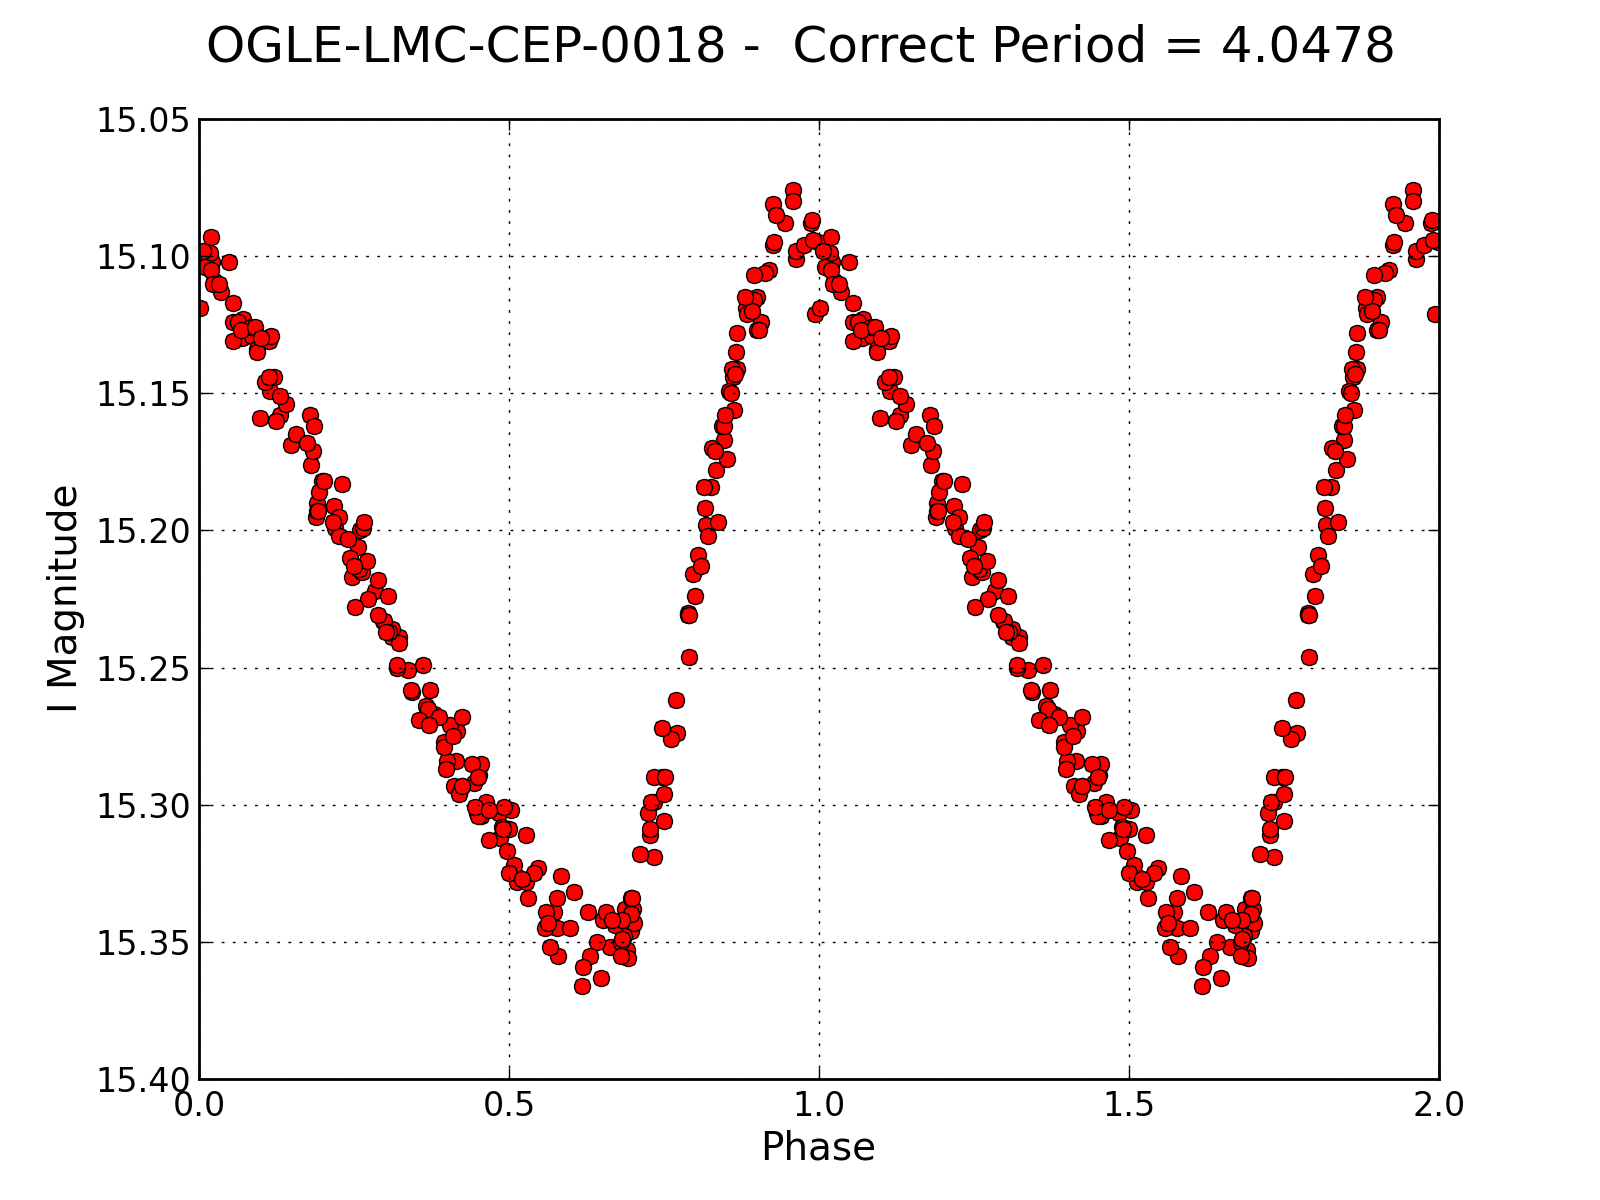
\includegraphics[width=\linewidth]{lightcurve_0018_correct_period.png}
%  \caption{Período correto}
%  \label{fig:right}
%\end{subfigure}%
%\begin{subfigure}{.5\textwidth}
%  \centering
%  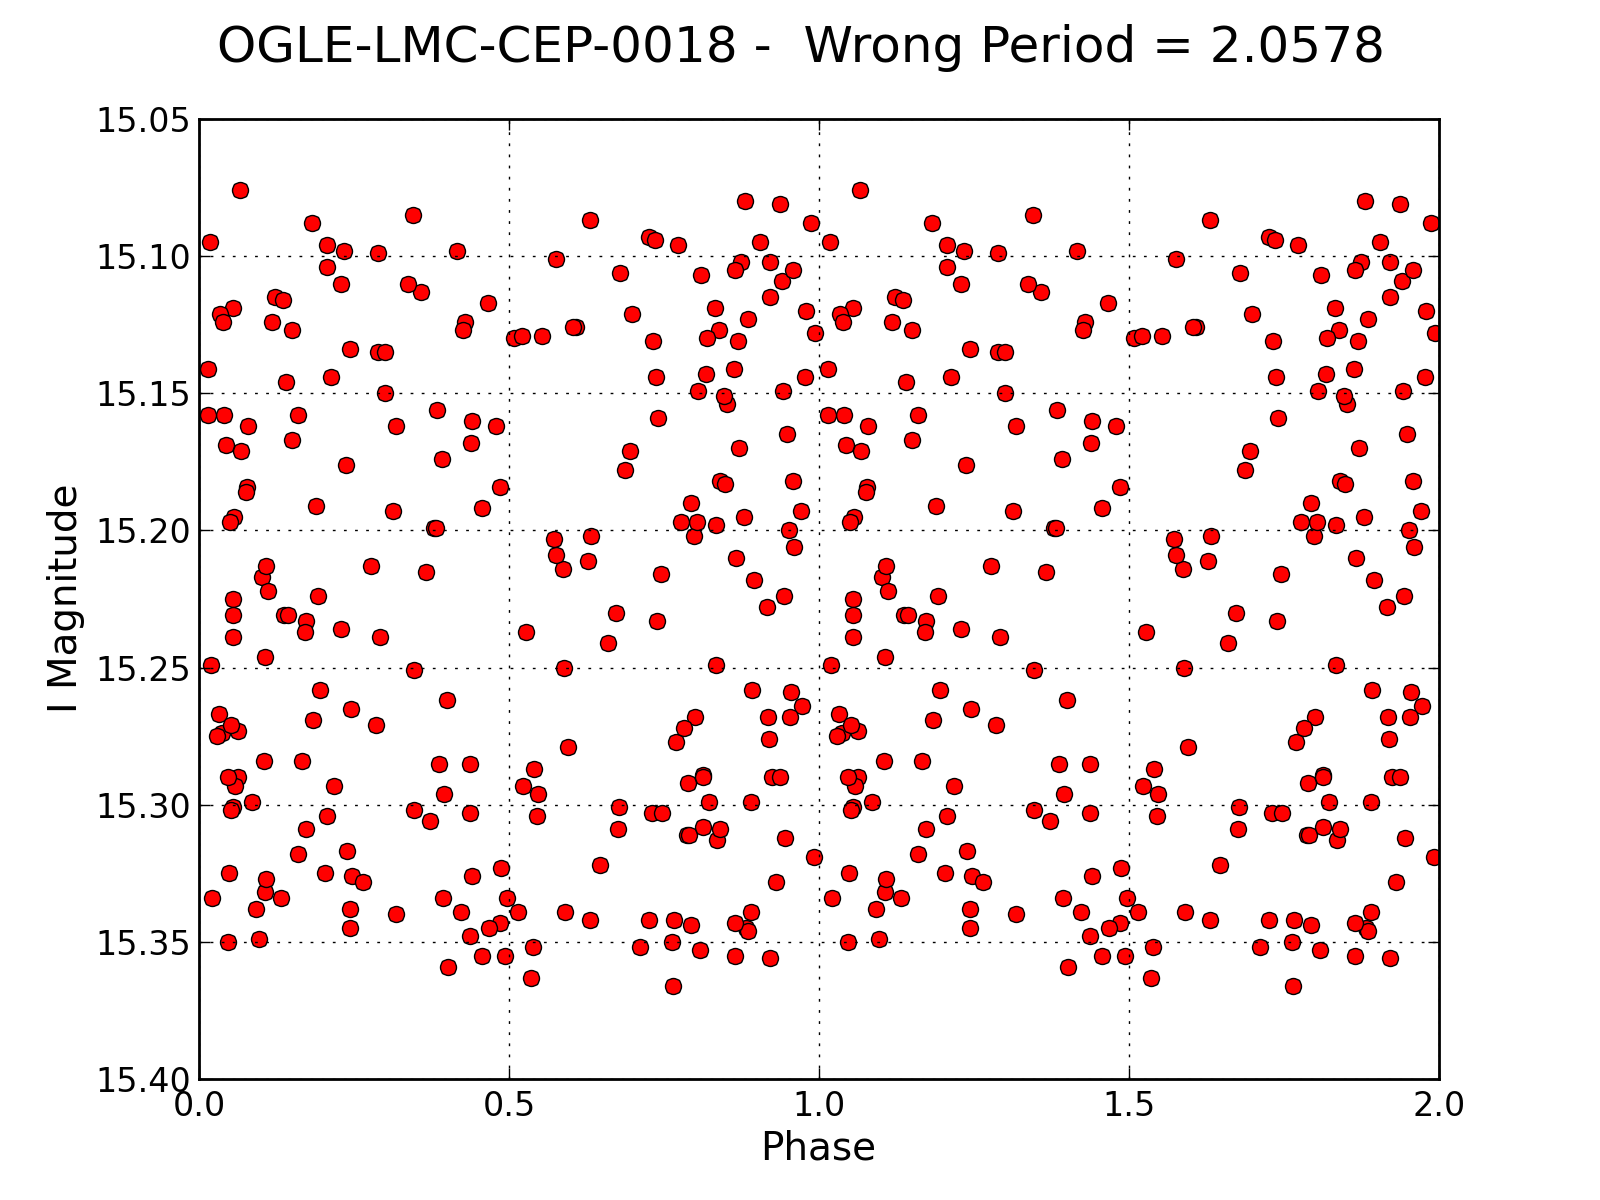
\includegraphics[width=\linewidth]{lightcurve_0018_wrong_period.png}
%  \caption{Período errado}
%  \label{fig:wrong}
%\end{subfigure}
%\caption{Exemplos de espa\c{c}o de fase}
%\label{fig:exemplo}
%\end{figure}
%
%Quando uma série temporal é dividida pelo período correto, será gerado uma dispersão com característica oscilante, como é o caso da figura \ref{fig:right}. Se o período utilizado na transforma\c{c}ão não for o correto, será gerado uma dispersão aleatória, sem forma definida, como mostra a figura \ref{fig:wrong}.
%
%\end{comment}

\section{Entropia de Shannon}

Na teoria de informação, a entropia ou entropia de Shannon \citep{informationTheory} é a medida de incerteza de uma variável. Em outras palavras, essa grandeza mede o grau de desordem para um sinal. Este sinal pode ser uma curva de luz ou até mesmo observações de velocidade radial de uma estrela \citep{entropy}. %A entropia de Shannon mede a falta de informação do nosso sistema, ou seja, quanto maior o seu valor mais incorreto a variável que estamos medindo. Desta forma, vamos procurar pela minimização da entropia no nosso espaço de fase.

O princípio deste método aplicado para a curva de luz de estrelas pulsantes se baseia na seguinte ideia: sendo sinais periódicos as curvas de luz das variáveis pulsantes, ao fazer a transformação para o espaço de fase, essa transformação com o período correto possui um certo grau de ordem, enquanto que a curva de luz construída com um período errôneo não possui ordem, gerando uma dispersão de pontos e todo o espaço de fase. Desta forma, a entropia de Shannon calculada para um sinal totalmente disperso em seu espaço de fase possui um valor maior do que essa mesma grandeza calculada para um sinal mais ordenado. Portanto, a entropia nos informa esse grau de desordem ou incerteza da variável em estudo, que neste caso é o período, e para um conjunto de períodos que queremos analisar a entropia de Shannon deve ser mínima para o período que produz a dispersão mais ordenada no espaço de fase. Um exemplo de espaço de fase com diferentes períodos é mostrado na figura \ref{fig:exemplo_entropia}.


\begin{figure}[!h]
\centering
\begin{subfigure}{.5\textwidth}
  \centering
  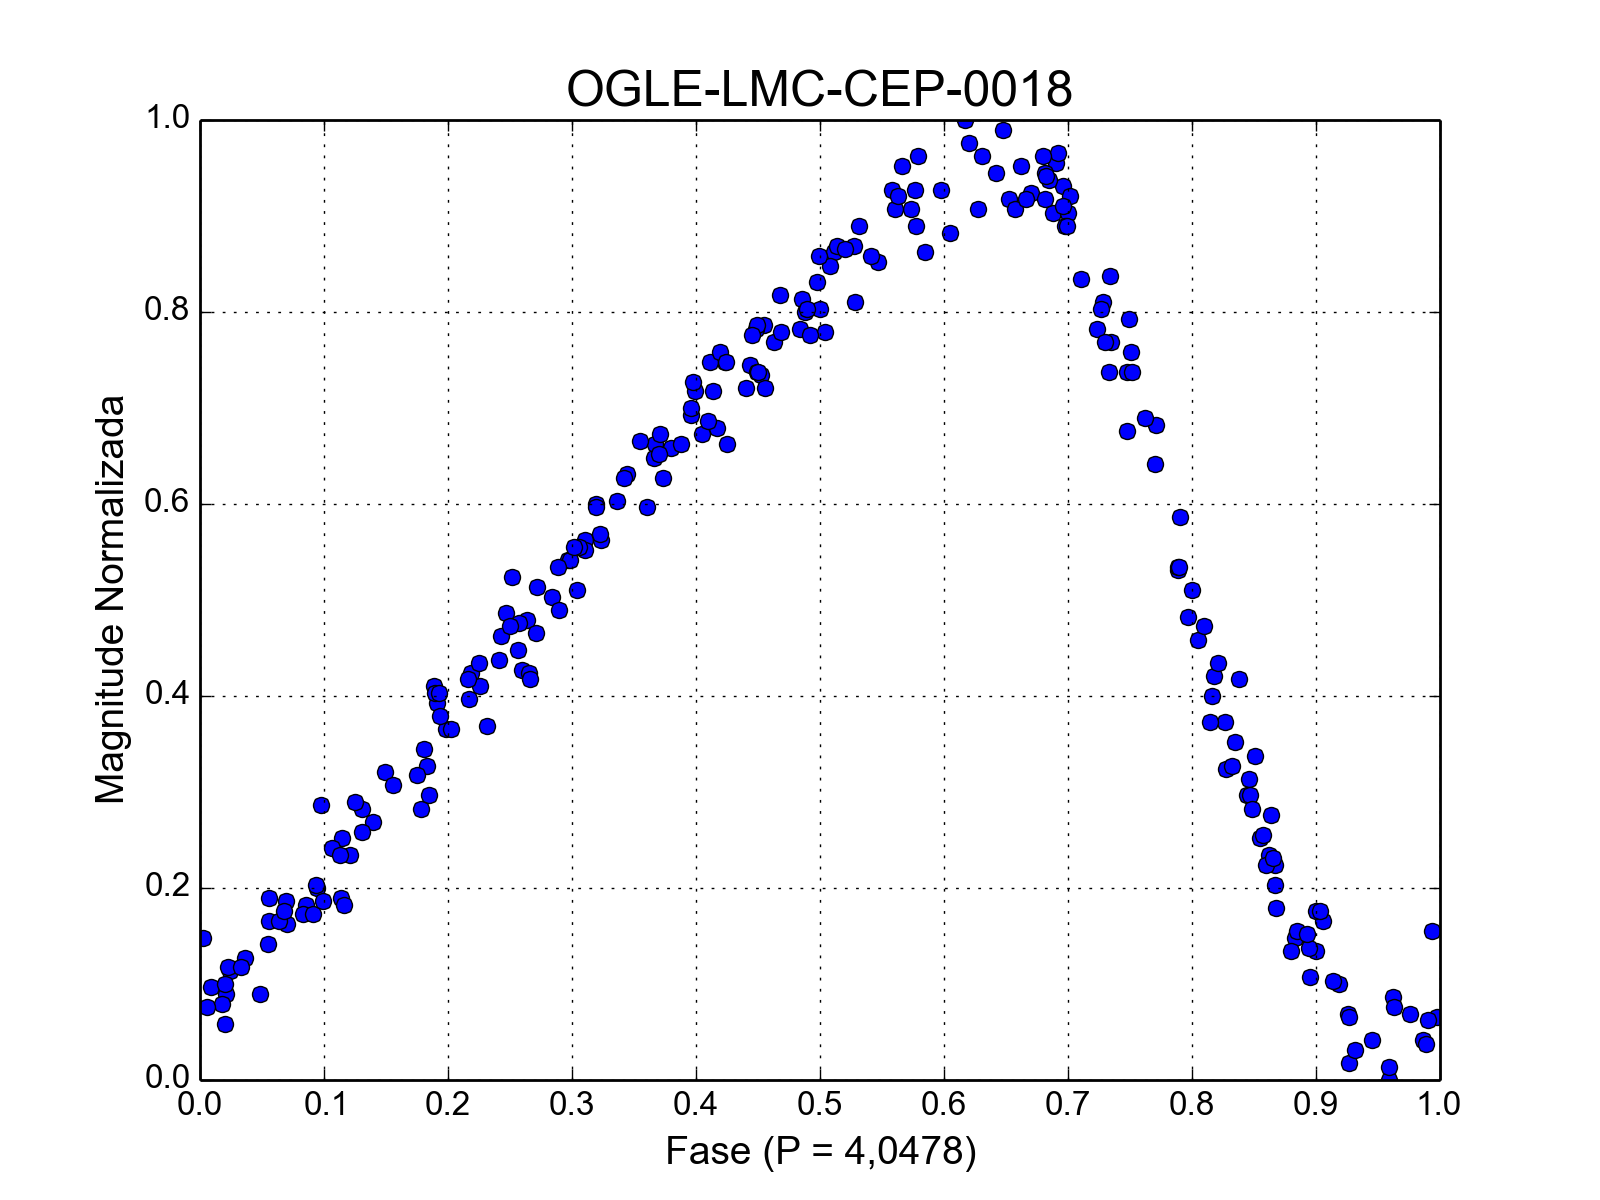
\includegraphics[width=\linewidth]{esp_fase_correto.png}
  \caption{Período correto}
  \label{fig:esp_fase_correto}
\end{subfigure}%
\begin{subfigure}{.5\textwidth}
  \centering
  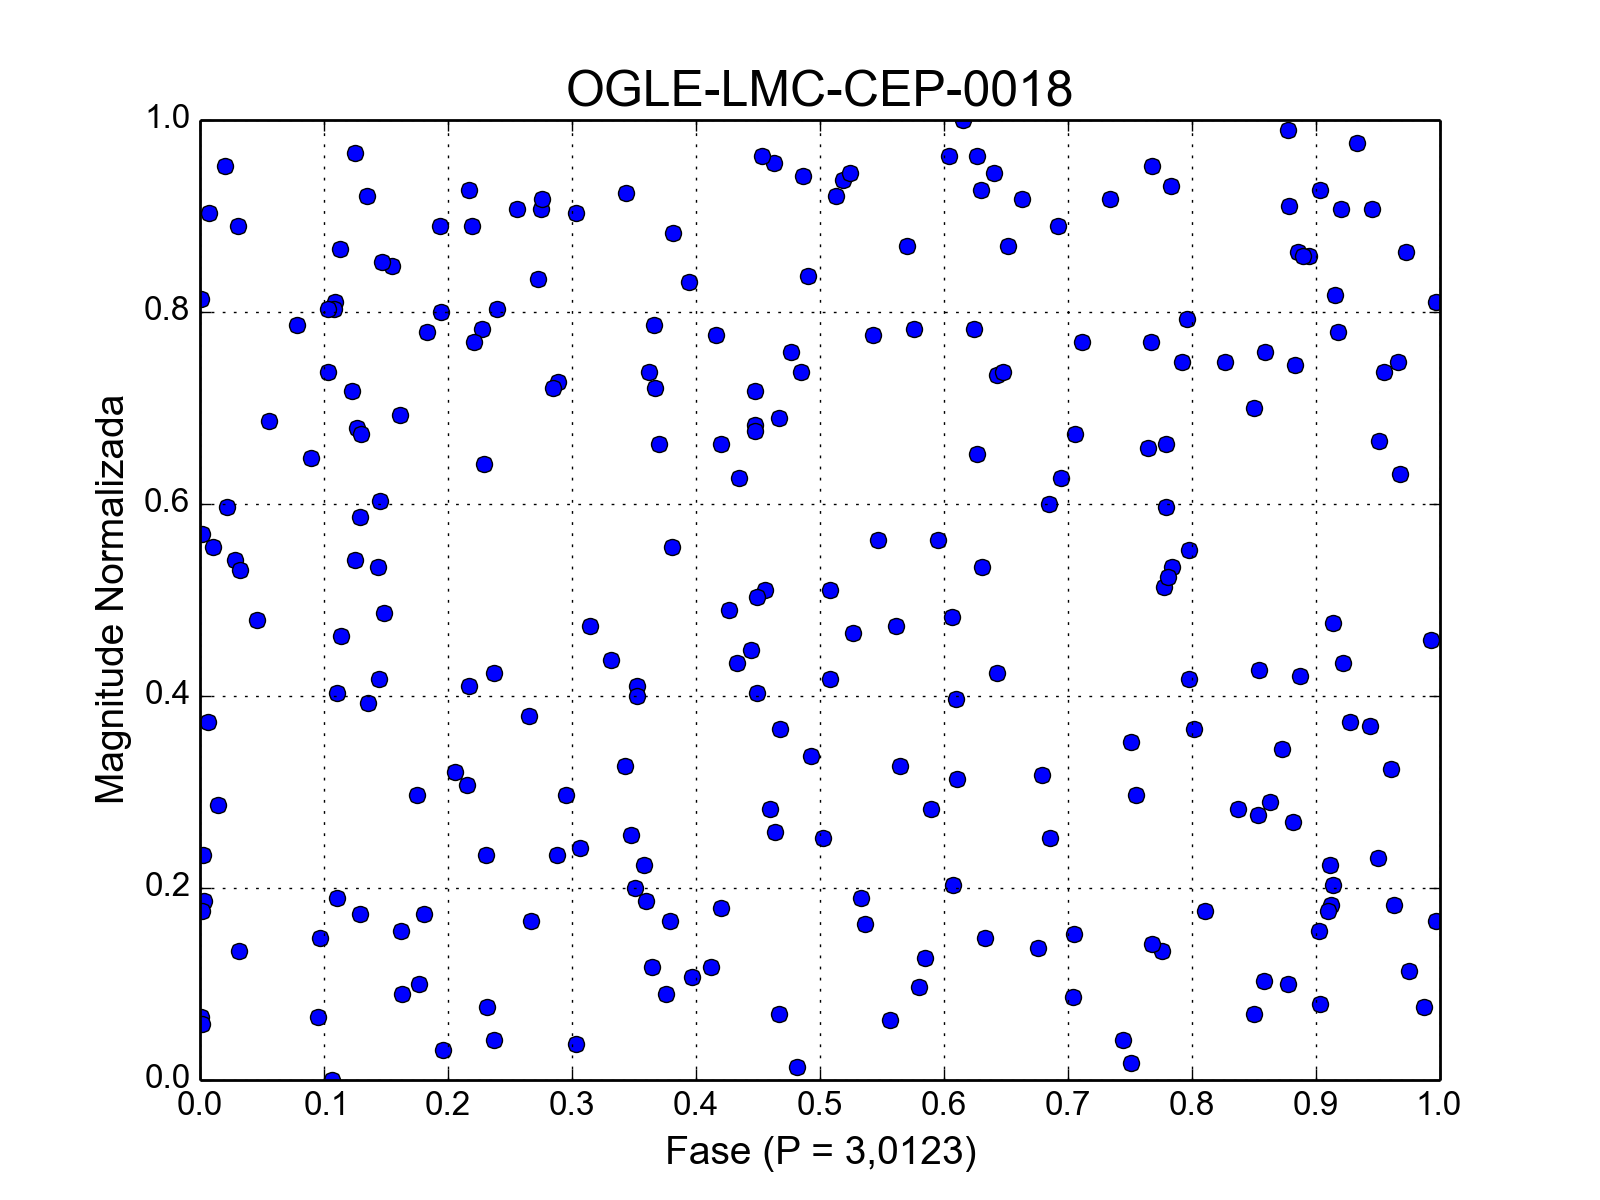
\includegraphics[width=\linewidth]{esp_fase_errado.png}
  \caption{Período errado}
  \label{fig:esp_fase_errado}
\end{subfigure}
\caption[Exemplos de entropia]{Exemplos da distribuição de pontos espaço de fase para a Cefeida OGLE-LMC-CEP-0018 do catálogo OGLE. O espaço de fase da imagem na esquerda foi construído utilizando o período correto ($P=4,0478$) e possui um valor para entropia de $H_c = 1,0762$. A imagem da direita foi utilizado um período aleatório ($P=3,0123$) e o valor de entropia calculado é $H_c = 1,5943$.}
\label{fig:exemplo_entropia}
\end{figure}


A entropia de Shannon foi aplicada pela primeira vez em curvas de luz por \citet{entropy}. Os autores normalizaram a magnitude das curvas de luz, transformaram para o espaço de fase e fizeram $m$ repartições nesse espaço. Desta forma, a entropia que é definida por:
\begin{align}
H = - \sum_i^m \mu_i \ln \mu_i
\end{align}
foi calculada. Nessa expressão, $\mu_i$ representa a probabilidade de ocupação da repartição $i$. Numericamente, a probabilidade de ocupação é calculada simplesmente contando os pontos de observação dentro da repartição e dividindo pela quantidade total de pontos. As vantagens desse método são a facilidade para lidar com sinais que possuam espaçamento variável entre os seu pontos, a simplicidade de aplicação e possui um embasamento matemático e estatístico bem definido dentro da teoria de informação, sendo que nem todos os métodos de detecção de períodos possuem esse ultimo item bem definido \citep{entropy}.


\subsection{Entropia condicional de Shannon }

A entropia de Shannon condicional surgiu da necessidade de contornar um problema bem conhecido da análise de curvas de luz: o efeito de \textit{Aliasing} causado pelo período $P=1$ dia. Este efeito ocorre devido as observações serem efetuadas sempre à noite, o que ocasiona um espaçamento de um dia entre os conjuntos de observação. A figura \ref{fig:periodo1dia} mostra a distribuição de pontos no espaço de fase normalizado utilizando o período $P=1$ dia. A entropia de Shannon calculada para uma distribuição desta forma retorna um valor pequeno, pois os pontos estão localizado em uma determinada parte do espaço.
\begin{figure}[!ht]
\centering
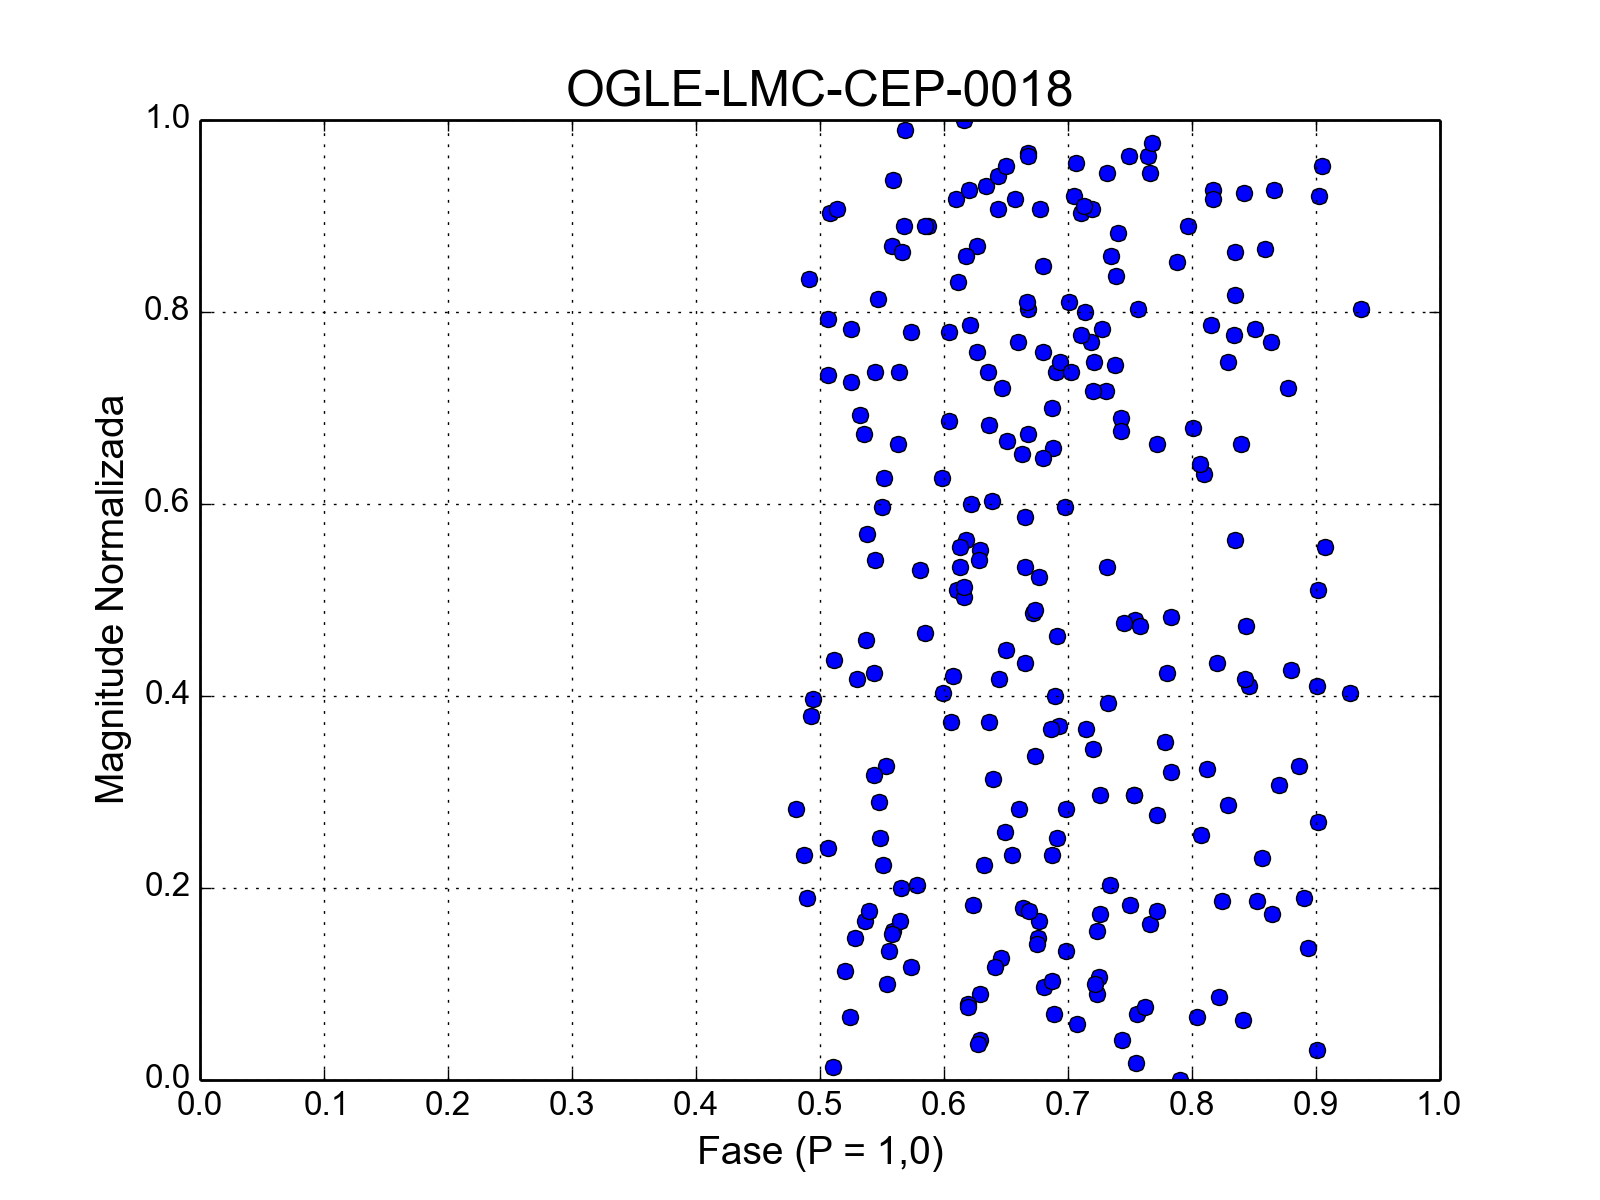
\includegraphics[width=0.5\linewidth]{esp_fase_1dia.png}
\caption[Efeito de \textit{Aliasing} com período de 1 dia.]{Efeito de \textit{Aliasing} devido ao período de 1 dia para a Cefeida OGLE-LMC-CEP-0018 do catálogo OGLE. Os pontos se localizam em uma determinada região do espaço de fase (menos da metade) o que faz com que a entropia calculada seja pequena. A entropia condicional foi proposta para lidar com este problema e para este caso o seu valor é $H_c=1,5542$.}
\label{fig:periodo1dia}
\end{figure}
Para lidar com esse problema, \citet{ce} propuseram a entropia de Shannon condicional. Nesta variação do método o espaço de fase é dividido em $i$ repartições na magnitude e $j$ repartições na fase e a entropia é calculada da seguinte forma:
\begin{align}
H_c = \sum_{i,j} p(m_i,\phi_j) \ln \left( \frac{p(\phi_j)}{p(m_i,\phi_j)} \right)
\end{align}
em que $p(m_i,\phi_j)$ é a probabilidade de ocupação na $i$-ésima repartição da magnitude e na $j$-ésima repartição da fase e $p(\phi_j)$ é a probabilidade de ocupação na $j$-ésima repartição da fase. Como estamos lidando com repartições retangulares:
\begin{align}
p(\phi_j) = \sum_i p(m_i,\phi_j)
\end{align}
ou seja, $p(\phi_j)$ é a soma das probabilidades na i-ésima coluna.

\citet{ce} analisaram o impacto no resultado da entropia causado pela quantidade de repartições e estimaram que $5$ repartições na magnitude ($\Delta m = 0,2$) e $10$ repartições na fase ($\Delta \phi = 0,1$) seriam ideais, pois quanto maior a quantidade dessas repartições mais recursos computacionais são necessários, e com essa escolha a entropia continua retornando bons resultados em pouco tempo.

Desta forma, a entropia de Shannon condicional será utilizada considerando $5$ repartições para a magnitude e $10$ para fase. Este método será aplicado para o espaço de fase normalizado para um conjunto de períodos que se quer analisar, calculando a entropia de Shannon condicional para cada espaço de fase criado para esse conjunto de períodos. O menor valor de entropia corresponde ao conjunto de pontos mais ordenado, o que seria o período correto da estrela \citep{ce} . Porém, antes de entrar em detalhes no algoritmo criado é necessário entender os dados utilizado no trabalho.


%\begin{comment}
%Quando uma estrela possui um comportamento periódico, a variação em sua magnitude é representada em ciclos iguais. Cada ciclo é uma fase. Se os ciclos são iguais, não importa qual ciclo nos estamos observando, apenas onde nos estamos no ciclo. Assim, o espaço de fase é uma representação de todos os ciclos observados em apenas uma fase, ou em apenas um ciclo. Assim, os pontos de sobrepõem e formam uma oscilação geral da estrela. Este espaço de fase é calculado pela seguinte expressão,
%\begin{equation}
%\phi_i = \frac{t_i}{P} - \Big[\frac{t_i}{P}\Big]
%\end{equation}
%em que $t_i$ é o i-ésimo dado do tempo, $P$ é o período de oscilação da magnitude e a quantidade entre colchetes representa apenas o numero inteiro da divisão.
%%Most of the entropy based methods are based on information entropy. In information theory, entropy is a measure of the uncertainty in a random variable. So, the entropy measures the lack of information of one variable.
%
%%Information theory based methods extract information from the probability density function and so include higher-order statistical moments present in the data whereas Fourier or analysis of variance techniques are based only on second-order statistical analyses. This implies that information theory brings better modeling of the underlying process and robustness to noise and outliers \citep{graB13}.
%
%
%%Para calcular a entropia condicional, primeiramente é necessário transformar os dados para o espa\c{c}o de fase e normalizar a luminosidade da estrela. Quando os dados são lidos pelo programa, ele gera dois vetores, um com os dados sobre o tempo e outro com os dados sobre a luminosidade da estrela. Para transformar o tempo em fase é necessário dividir cada um dos elementos do vetor tempo pelo período e subtrair o inteiro desta divisão,
%%\begin{equation}
%%\phi_i = \frac{t_i}{P} - \Big[\frac{t_i}{P}\Big]
%%\end{equation}
%%assim, temos um novo vetor com os dados da fase. O gráfico que pode ser obtido com os dados da fase e da luminosidade representa a dispersão da série temporal no espa\c{c}o de fase. A entropia condicional é calculada a partir desta dispersão.
%
%%Um exemplo de espa\c{c}o de fase é dado a seguir:
%
%\begin{figure}[h!]
%\centering
%\begin{subfigure}{.5\textwidth}
%  \centering
%  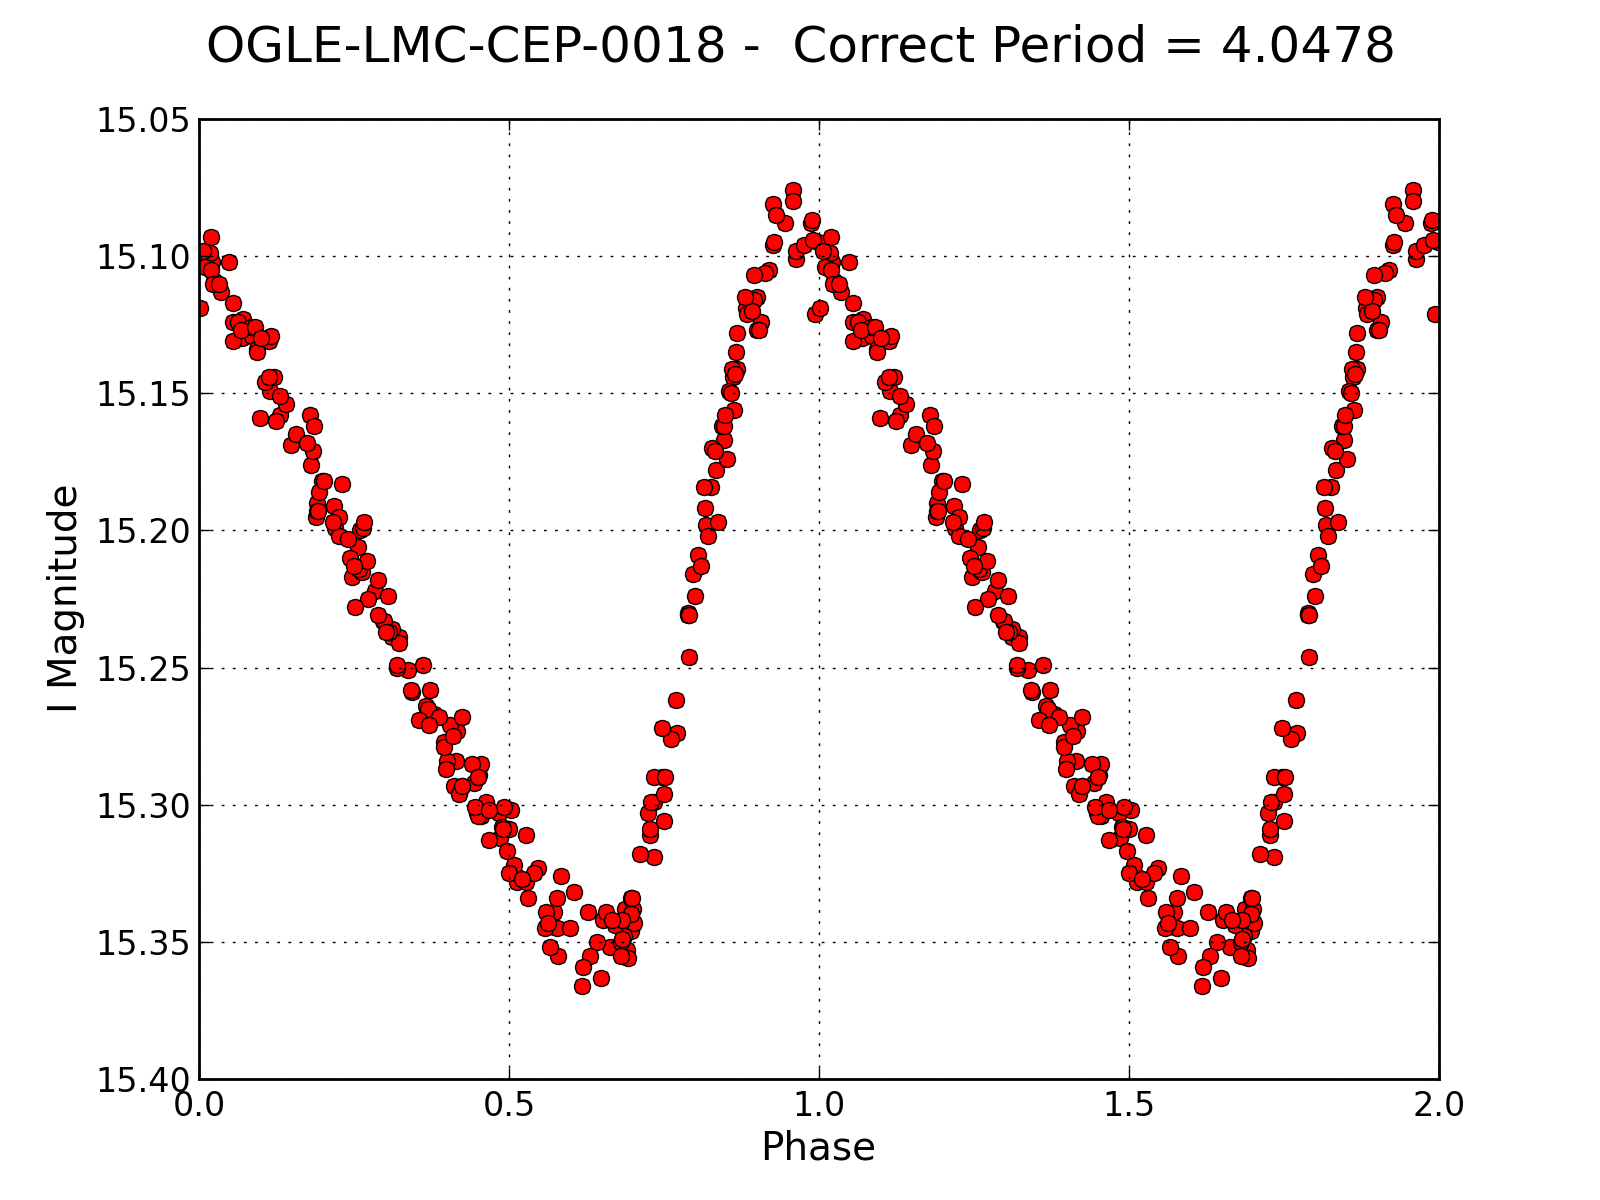
\includegraphics[width=\linewidth]{lightcurve_0018_correct_period.png}
%  \caption{Período correto}
%  \label{fig:right}
%\end{subfigure}%
%\begin{subfigure}{.5\textwidth}
%  \centering
%  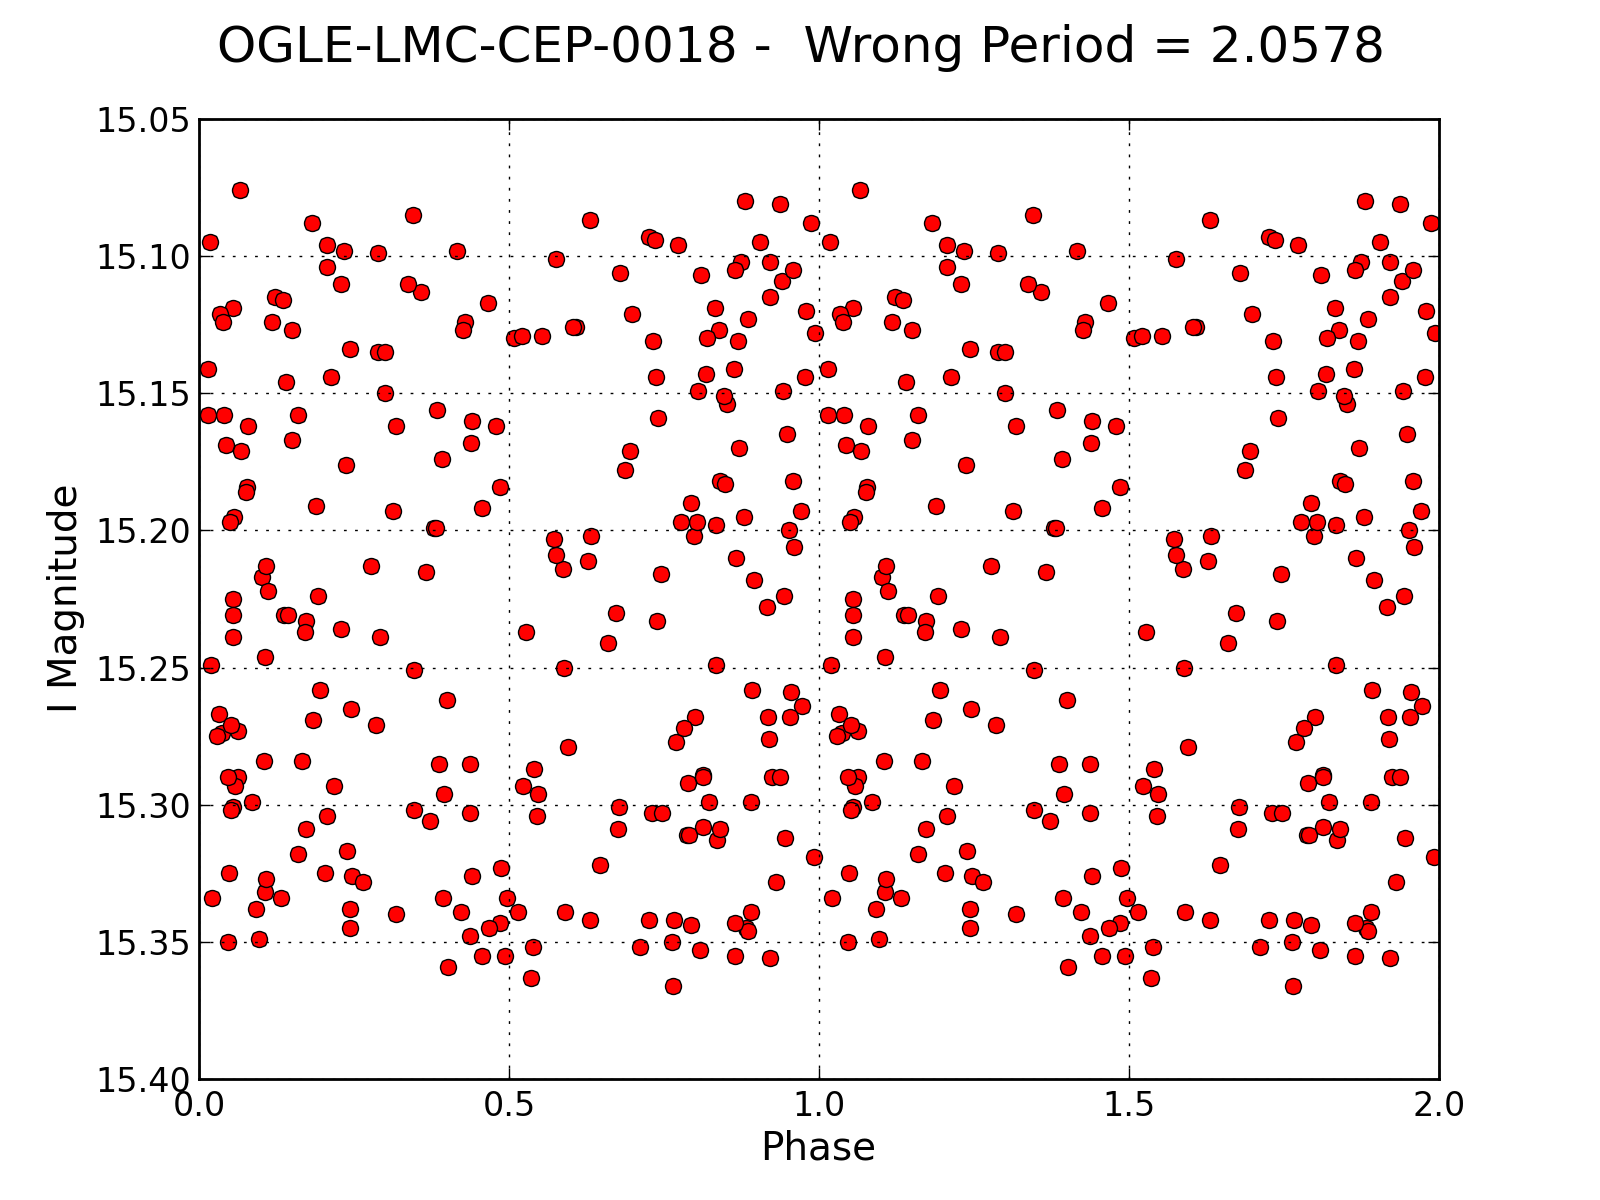
\includegraphics[width=\linewidth]{lightcurve_0018_wrong_period.png}
%  \caption{Período errado}
%  \label{fig:wrong}
%\end{subfigure}
%\caption{Exemplos de espa\c{c}o de fase}
%\label{fig:exemplo}
%\end{figure}
%
%Quando uma série temporal é dividida pelo período correto, será gerado uma dispersão com característica oscilante, como é o caso da figura \ref{fig:right}. Se o período utilizado na transforma\c{c}ão não for o correto, será gerado uma dispersão aleatória, sem forma definida, como mostra a figura \ref{fig:wrong}.
%
%\end{comment}

%Podemos observar que, no caso da figura \ref{fig:right}, os pontos se sobrepõem e formam uma curva. Assim, fazendo reparti\c{c}ões no dimensão da fase e da magnitude, podemos calcular a probabilidade dos pontos estarem localizados em cada um dos quadrados formados por estas reparti\c{c}ões em rela\c{c}ão a coluna em que eles estão e somá-los para obter uma grandeza. Esta grandeza é a entropia condicional, que é calculada pela seguinte formula \citep{ce},
%
%\begin{equation}
%H_c = \sum_{i,j} p(m_i,\phi_j)\ln \Big(\frac{p(\phi_j)}{p(m_i,\phi_j)}\Big)
%\end{equation}
%onde $p(m_i,\phi_j)$ é a probabilidade de ocupa\c{c}ão na $i$-ésima reparti\c{c}ão da magnitude e na $j$-ésima reparti\c{c}ão da fase e $p(\phi_j)$ é a probabilidade de ocupa\c{c}ão na $j$-ésima reparti\c{c}ão da fase. No caso de reparti\c{c}ões retangulares, %a probabilidade de ocupa\c{c}ão
%\begin{equation}
%p(\phi_j) = \sum_i p(m_i,\phi_j)
%\end{equation}

%A entropia de Shannon mede a falta de informa\c{c}ão do sistema, ou seja, quanto maior o seu valor, mais incorreto o período. Por isso que buscamos a minimiza\c{c}ão da entropia.
%Considerando estes dois exemplos, a probabilidade de de ocupa\c{c}ão das reparti\c{c}ões é menor na figura \ref{fig:right} do que na figura \ref{fig:wrong}. O menor valor de entropia condicional é associado ao período mais provável da estrela \citep{ce}.


\section{Catálogo OGLE}

O catálogo OGLE (\textit{The Optical Gravitational Lensing Experiment}) \citep{Udalski2008} consiste em 8 anos de dados observacionais cobrindo uma área de 40 graus quadrados na direção das Nuvens de Magalhães. Esse catálogo busca por estrelas variáveis tendo monitorado mais de 200 milhões de estrelas. As observações foram feitas utilizando os filtros Cousins I e V \citep{Cousins1973}. Na banda I, as observações possuem um tempo de $180 \si{s}$ de exposição tendo em média 400 medidas de observação. Por outro lado, a banda V possui em média apenas 30 medidas de observação. Os dados da sua terceira fase \citep{Udalski2008}, chamado de OGLE-III, são públicos\footnote{\url{http://ogledb.astrouw.edu.pl/~ogle/CVS/}} e foram utilizados nesse trabalho, dando prioridade para as observações na banda I devido a maior quantidade de medidas em relação a banda V.

Os dados de observação disponíveis são obtidos no formato .dat e possuem três colunas que significam tempo em dias Julianos, magnitude e erro na magnitude. Um exemplo de dado pode ser visto na tabela \ref{tab:dados}.

\begin{table}
\begin{center}
%\captionof{table}{Exemplo de dados}
\caption{Exemplo de dados do catálogo OGLE}
\begin{tabular}{c|c|c}
\toprule
Tempo & Magnitude & Erro \\
\midrule
2165,85271 & 15,130 & 0,007 \\
%\hline
2183,83450 & 15,326 & 0,008 \\
2238,62899 & 15,102 & 0,007 \\
$\vdots$ & $\vdots$ & $\vdots$ \\
\bottomrule
\end{tabular}
\label{tab:dados}
\end{center}
\end{table}

Nesse trabalho foram utilizados os dados de dois tipos de estrelas variáveis pulsantes localizadas na Grande Nuvem de Magalhães, as Cefeidas Clássicas e as RR Lyraes, sendo utilizados $3056$ Cefeidas classificadas entre modo fundamental (FU) e primeiro sobretom (FO) e $22651$ RR Lyraes também classificas entre modo fundamental (AB) e primeiro sobretom (C), totalizando $25707$ estrelas.

%We selected RRab stars from OGLE-III catalog that con- sists of 8-year archival data identified and characterized by the Fourier coefficients of the light curves (SZ09). The cat- alog contains 17, 693 RRab stars having a mean period of < Pab >= 0.576 days. The OGLE field in the LMC cov- ers nearly 40 deg2. Most of the observations were carried out using the Cousins I-band filter with exposure time of 180s having an average of 400 photometric observations. The catalog also contains V -band light curves of 17, 337 stars having an average of 30 data points per light curve. The



\section{Algoritmo}

Foi desenvolvido um algoritmo em \texttt{Python3} para calcular a entropia condicional de dados de estrelas variáveis pulsantes  pertencentes ao Catálogo OGLE-III. A figura \ref{alg:algoritmo} apresenta um pseudo-código do algoritmo. O código completo é apresentado no apêndice \ref{apend:algoritmo}. %\href{http://ogledb.astrouw.edu.pl/~ogle/CVS/}{Catálogo OGLE-III de estrelas variáveis}. %Os dados são obtidos no formato .dat e possuem três colunas que significam tempo, magnitude e erro. Um exemplo de arquivo pode ser visto na tabela \ref{tab:dados}.

\begin{algorithm}[!h]
\SetAlgoLined
\Entrada{Tempo e Magnitude \\
\Saida{Período $P$ que minimiza a entropia}
\Inicio{
Leitura dos dados de entrada como vetores; \\
Cria um vetor com $n$ períodos sendo P = ($p_1$ , $p_2$, $\cdots$, $p_n$); \\
Normalização da magnitude;\\
%\ParaCada{$p_i$ com $i = 1$  \Ate $i =n$}{
\ParaCada{$p_i$ em $P$}{
Transformar o tempo para o espaço de fase; \\
Faz as repartições e contabiliza os pontos; \\
Calcula a entropia de Shannon condicional; \\
Armazena a entropia calculada para o período $p_i$
}
Achar o valor mínimo de entropia: $E_{min}$ = min(Entropia) \\
Achar o período que minimiza a entropia:
$P_{E_{min}}$=P[min(entropia)]
}
\Retorna{$P_{E_{min}}$}
}
\caption[Pseudo-código do algoritmo.]{Pseudo-código do algoritmo em português estruturado.}
\label{alg:algoritmo}
\end{algorithm}

Para cada um dos dados das estrelas que serão analisadas, o programa faz a leitura das informações de tempo e magnitude da estrela, criando um vetor de períodos que serão analisados. Para uma Cefeida, esse vetor de períodos é criado com período inicial $p_1 = 0,1$ dias e período final $p_n = 32$ dias, com um intervalo entre os períodos de $0,001$ dia. Então, para cada um dos elementos do vetor período o algoritmo faz as seguintes ações: o tempo é transformado em fase, são feitas as repartições no espaço de fase e são contabilizados a quantidade de pontos em cada repartição; a entropia de Shannon condicional é calculada e o valor armazenado em um vetor entropia. % O mesmo é feito para o próximo período do vetor período até que sejam calculados a entropia para todos os dados deste vetor.
No fim, o algoritmo indica o menor valor do vetor entropia e qual período esta relacionado com este valor. %A figura \ref{fig:flow} apresenta um fluxograma do algoritmo.

%\begin{figure}[!hb]
%\centering
%	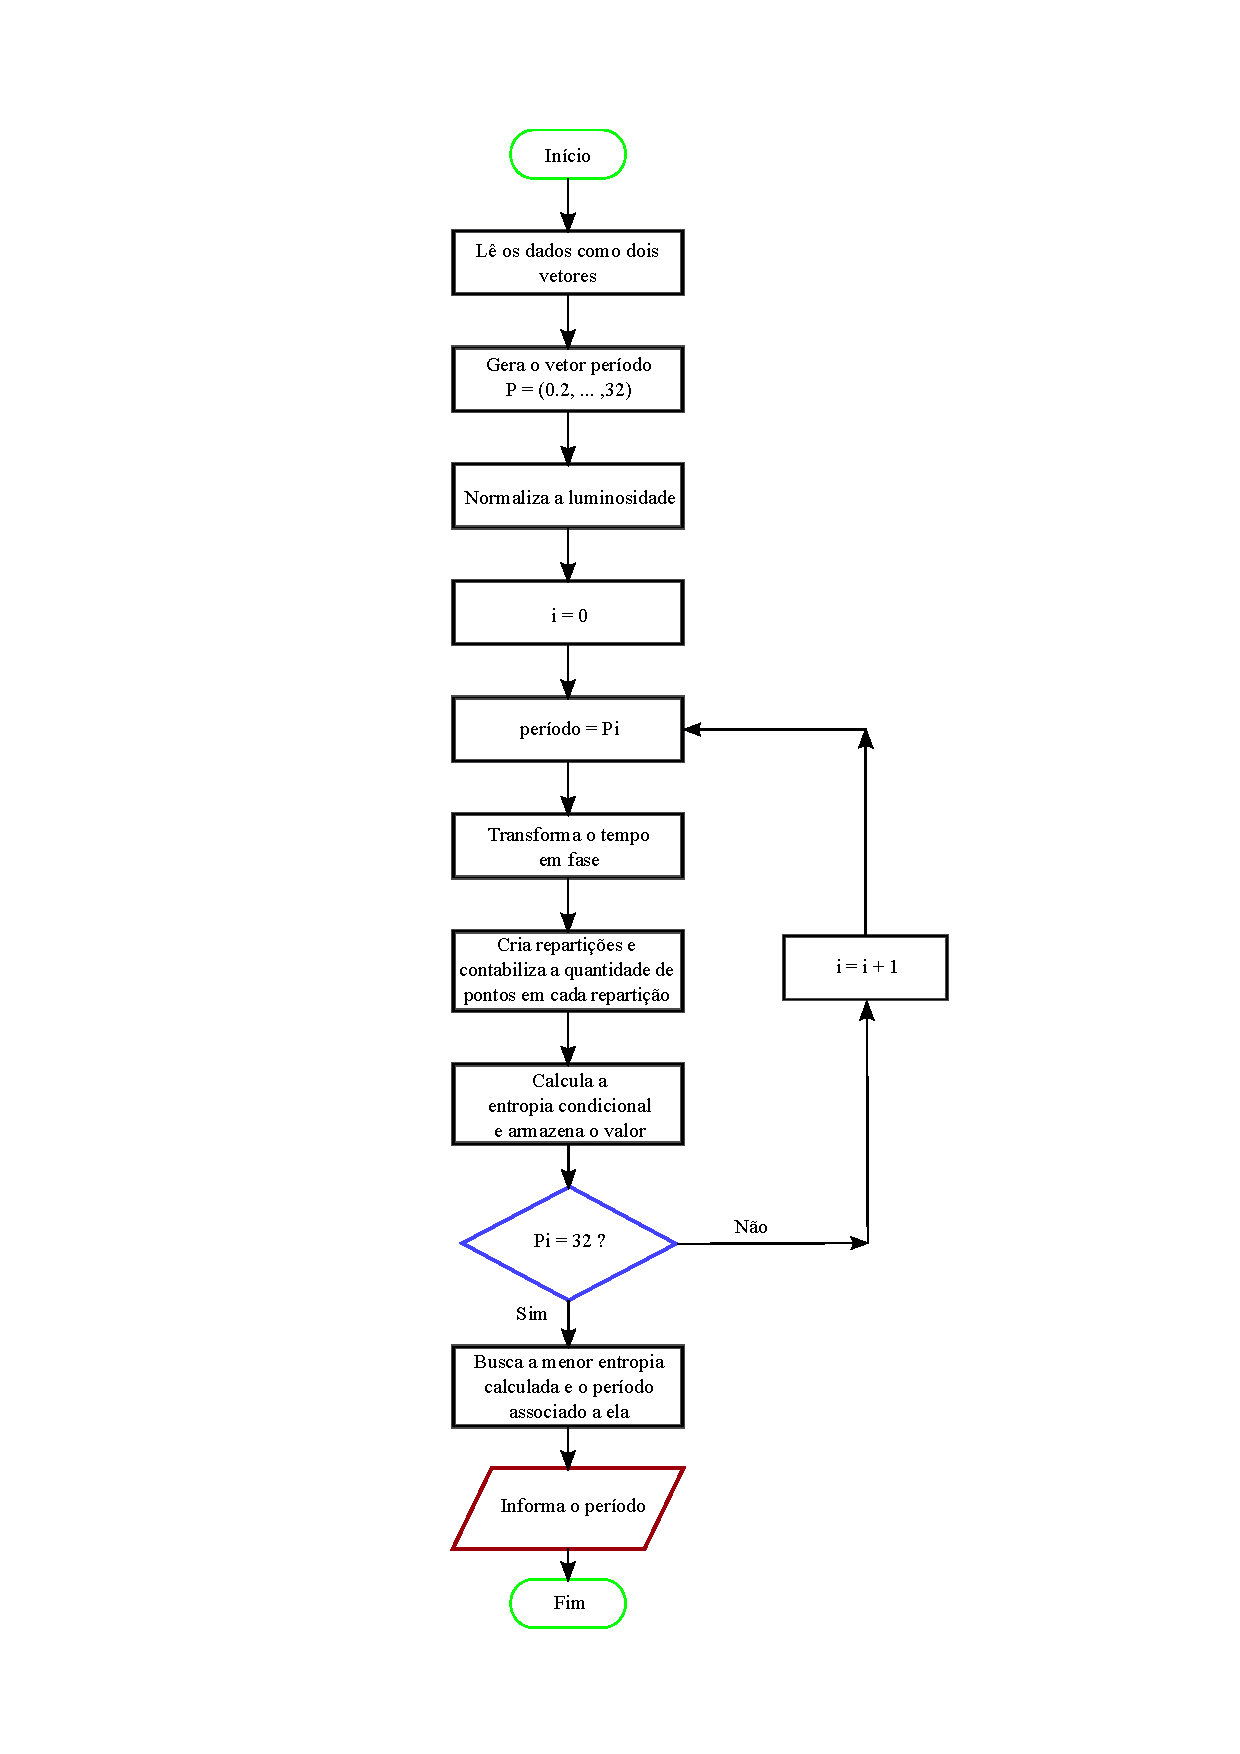
\includegraphics[scale=.6]{drawing.pdf}
%	\caption{Fluxograma do algoritmo}
%	\label{fig:flow}
%\end{figure}

\section{Análise Teórica}

Ao aplicar o algoritmo nos dados do catálogo podemos analisar como o método responde para dados reais. Porém, se quisermos analisar qual a abrangência de atuação desta técnica, é possível calcular a entropia de Shannon para um conjunto de dados teóricos em que seja conhecido o período. Desta forma, podemos entender como o formato de um sinal influencia nos resultados finais.

De acordo com %a literatura,
\citet{ce} e \citet{entropy}, um sinal periódico sintético que se assemelhe com os dados observacionais da maioria dos Surveys de estrelas variáveis pode ser construído utilizando a expressão:
\begin{align}
m(t) = A_0 + \sum_{i=1}^3 A_i \sin \left( \frac{2 k \pi t}{P} \right) + B \eta \label{eq:dado_sint}
\end{align}
Em que $m(t)$ é a magnitude sintética, $A_0$ é termo de deslocamento linear, os termos $A_i$ são termos de escala para as funções senos, $k$ é um parâmetro de escala para a amostragem do sinal, $t$ é o vetor tempo, $P$ é o período de oscilação do sinal, $\eta$ é uma distribuição gaussiana com média zero e desvio unitário que tem como função introduzir ruído no sinal e $B$ é um parâmetro de escala para esse ruído.

A amostragem ($f_s$) de um sinal representa a frequência de pontos de observação. Essa quantidade afeta diretamente a construção do vetor tempo, pois a amostragem é definida como:
\begin{align}
f_s = \frac{1}{dt} \quad \to \quad dt = \frac{1}{f_s} \label{eq:amostragem}
\end{align}
Ou seja, o intervalo de tempo depende do valor da amostragem. Desta forma, assim que for definida a nossa amostragem, podemos variar essa grandeza para construir os vetores tempos e com isso construir o sinal sintético para calcular a entropia de Shannon condicional e analisar os resultados. A análise de todos os dados, sintéticos e reais, será discutida no capítulo \ref{cap:resultados}.

%!TEX root = /home/glauffer/Dropbox/FURG/final_project/monografia/monografia.tex
\chapter{Resultados e Discussão}
\label{cap:resultados}
%Como mostrar os resultados de maneira eficiente

%\section{resultado parciais}
\section{Dados do Catálogo OGLE}

Em um total foram calculados os períodos de $25707$ estrelas variáveis localizadas na Grande Nuvem de Magalhães e pertencentes ao catálogo OGLE. Deste numero total, $3056$ eram Cefeidas clássicas tipo FO e FU, e $22651$ eram RRLyraes tipo AB e C. Os resultados obtidos foram comparados com os resultados do catálogo e o percentual de acertos, considerando uma precisão de $10^{-4}$, pode ser visto na tabela \ref{tab:resultados}.

\begin{table}
\begin{center}
\caption[Quantidade de dados analisados e resultados corretos.]{Quantidade de dados analisados e resultados corretos considerando uma precisão de $10^{-4}$.}
\begin{tabular}{c|c|c|c}
\toprule
Estrelas & Quantidade & Acertos  & Porcentagem \\
\midrule
Cefeidas FU & $1818$ & $1817$ & $99,94 \%$ \\
Cefeidas FO & $1238$ & $1231$ & $99,43 \%$ \\
%\hline
RRLyraes AB& $17693$ & $17540$ & $99,14 \%$ \\
RRLyraes C& $4958$ & $4535$ & $91,47 \%$ \\
\midrule
\textbf{Total} & $\textbf{25707}$ & $\textbf{25123}$ & $\textbf{97,73 \%}$ \\
\bottomrule
\end{tabular}
\label{tab:resultados}
\end{center}
\end{table}

De acordo com os resultados da tabela \ref{tab:resultados} podemos perceber que para as Cefeidas o método apresenta um resultado um pouco melhor se comparado com as RR Lyraes. Uma explicação para este resultado seria que o método de entropia de Shannon condicional funciona melhor para magnitudes mais brilhantes \citep{comparison}. Tendo em vista que as Cefeidas ($m \approx 15$) são mais brilhantes do que as RR Lyraes ($m \approx 19$), essa afirmação é coerente com os resultados. %e sendo as Cefeidas ($m \approx 15$) mais brilhantes do que as RR Lyraes ($m \approx 19$), essa afirmação é coerente com os resultados.  %ver faixa de magnitude da cefeidas e lyraes

A alta taxa de acerto do método nos informa que
com estes resultados podemos confiar no método de entropia de Shannon condicional, porém para entender melhor o comportamento desse método será analisado os resultados para dados sintéticos.

\section{Dados Sintéticos}

Dados sintéticos foram criados a fim de explorar o método e entender até onde podemos utilizá-lo, pois os sinais sintéticos são construídos com parametros que podemos controlar e modificar. De acordo com a tabela \ref{tab:resultados}, as RRLyraes apresentaram uma taxa menor de acerto, por essa razão elas foram utilizadas como referencia para construir os dados sintéticos. Para isto, é necessário entender os dados das RR Lyraes do catálogo OGLE para obter os parâmetro sobre o tempo e amostragem para enfim utilizar a expressão \ref{eq:dado_sint} e construir os dados.

Analisando os dados das $22651$ estrelas, foram criados histogramas sobre os dados iniciais e finais do tempo e a quantidade de pontos de observação. As figuras \ref{fig:hist} e \ref{fig:histo_n} nos mostram esses histogramas.

\begin{figure}[!h]
\centering
\begin{subfigure}{.5\textwidth}
  \centering
  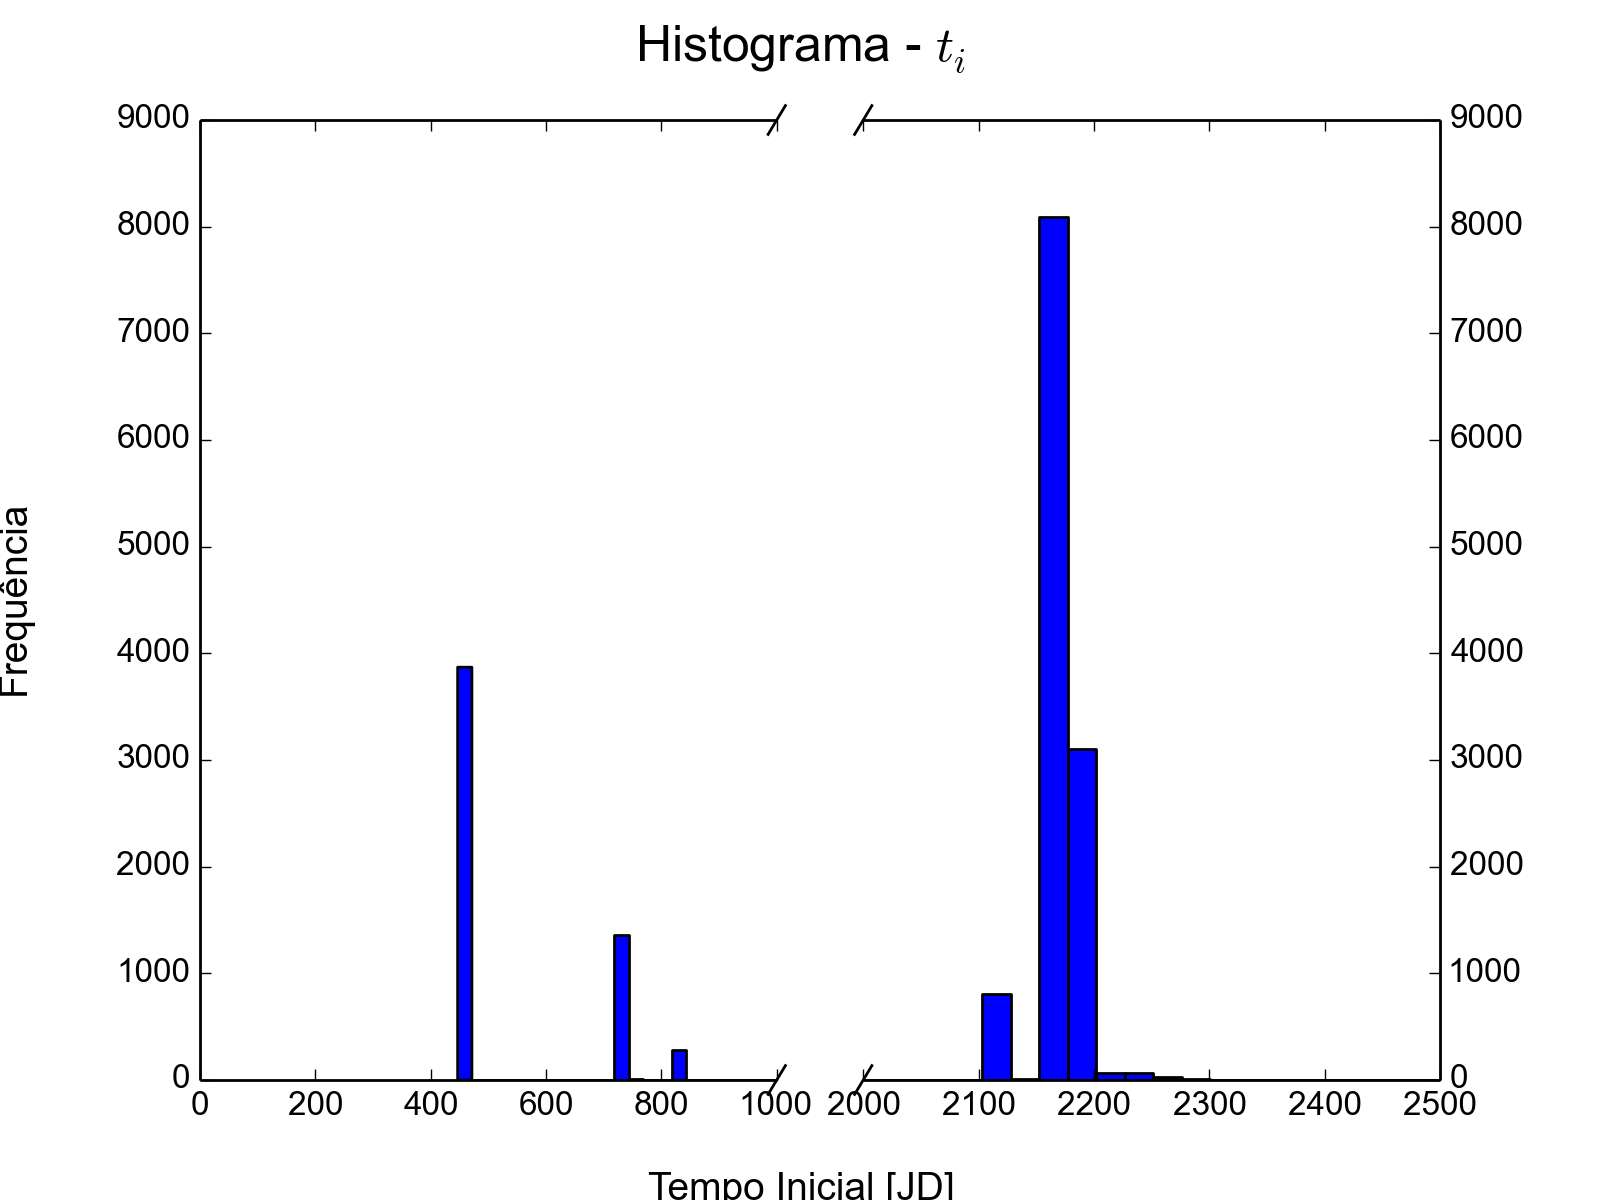
\includegraphics[width=\linewidth]{hist_ti.png}
  \caption{Tempo Inicial}
  %\label{fig:right}
\end{subfigure}%
\begin{subfigure}{.5\textwidth}
  \centering
  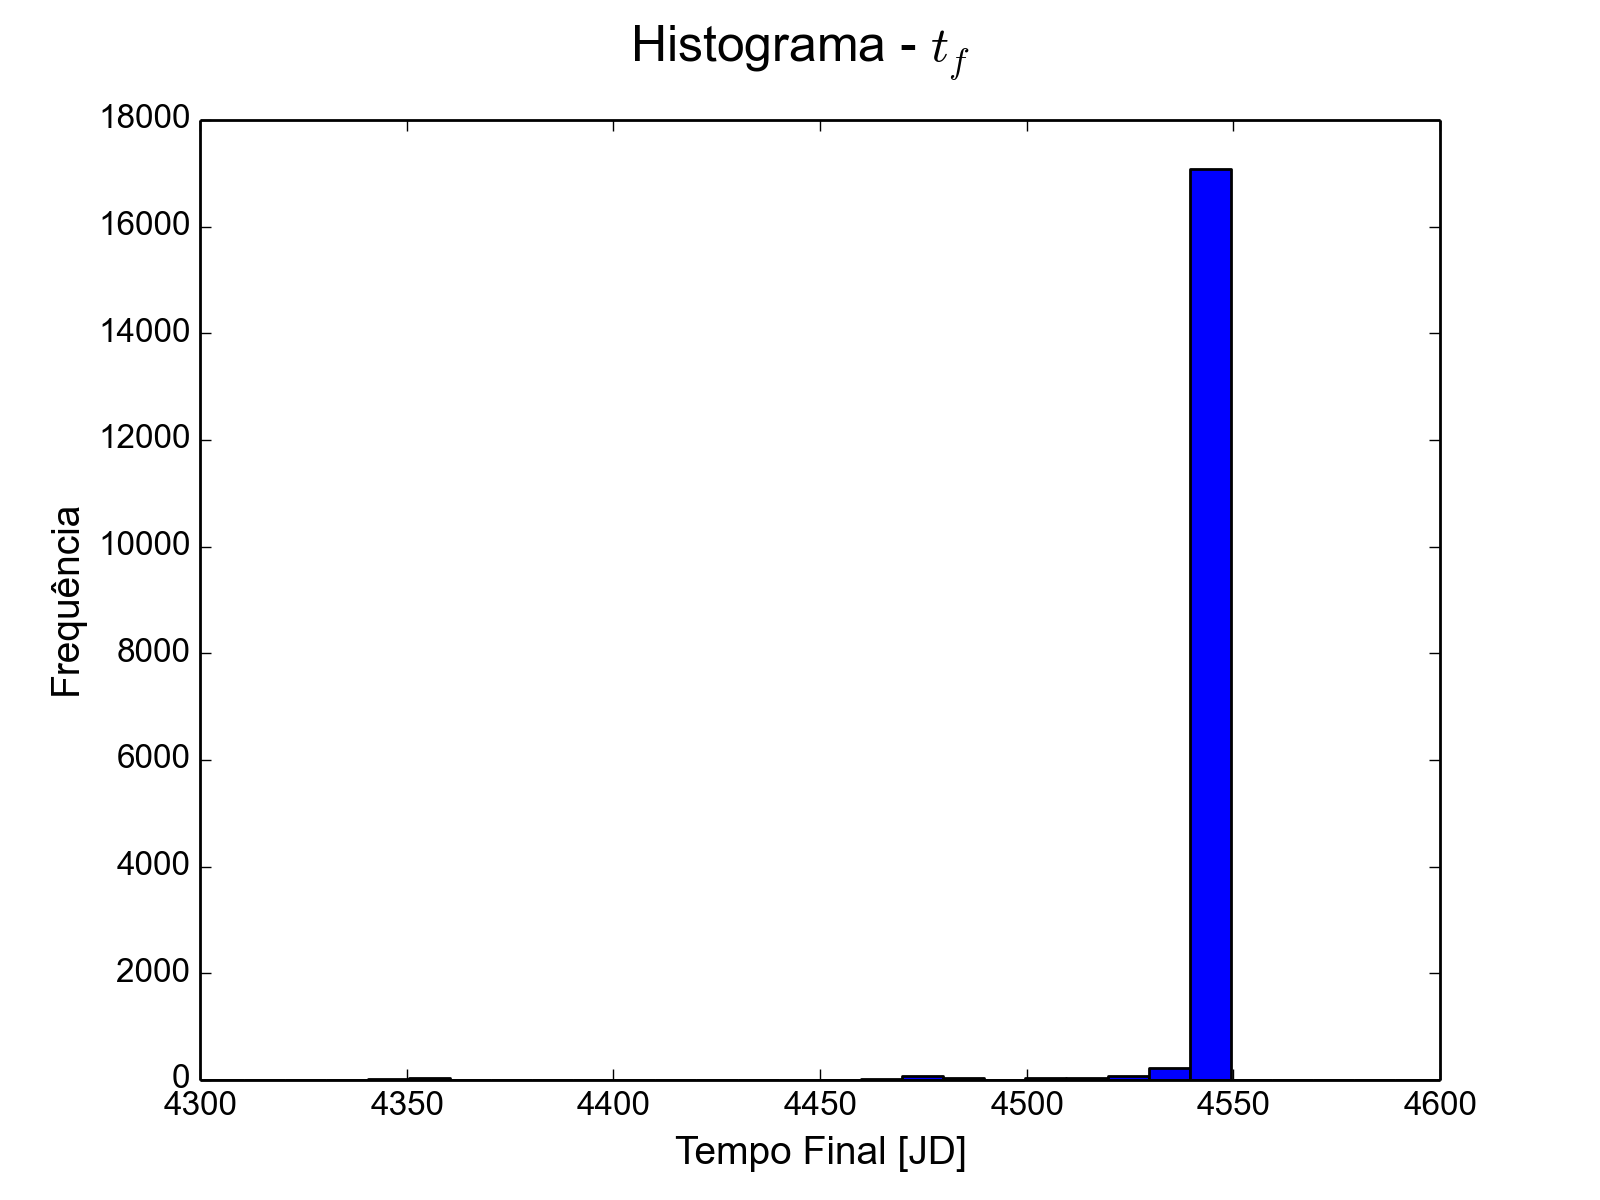
\includegraphics[width=\linewidth]{hist_tf.png}
  \caption{Tempo Final}
  %\label{fig:wrong}
\end{subfigure}
\caption[Histogramas sobre tempo inicial e final.]{Histogramas sobre o tempo inicial e final das RR Lyraes. As imagens representam (a) tempo inicial e (b) tempo final . A partir dessa análise foram obtidos os valores $t_i = 2152,5019$ e $t_f = 4539,4593$.}
\label{fig:hist}
\end{figure}

A partir dessa análise foram obtidos os valores $t_i = 2152,5019$ e $t_f = 4539,4593$ e $n = 352$ como os valores de tempo inicial, final e quantidade de pontos mais frequentes nos dados das RR Lyraes. Desta forma, utilizando esses valores é possível construir um sinal sintético que se assemelhe com os dados do catálogo. Então, a amostragem é calculada pela expressão \ref{eq:amostragem} em que a variação do tempo é obtida da seguinte forma:
\begin{align}
dt = \frac{t_f - t_i}{n} = \frac{4539,4593 - 2152,5019}{352} = 6,7888
\end{align}
E substituindo este resultado na equação \ref{eq:amostragem} teremos:
\begin{align}
f_s = 0,1473 .
\end{align}
Desta forma foi determinado, a partir dos dados do catálogo, qual a variação média entre os pontos de observação e foi calculada a amostragem média dos dados.

\begin{figure}[!ht]
  \centering
  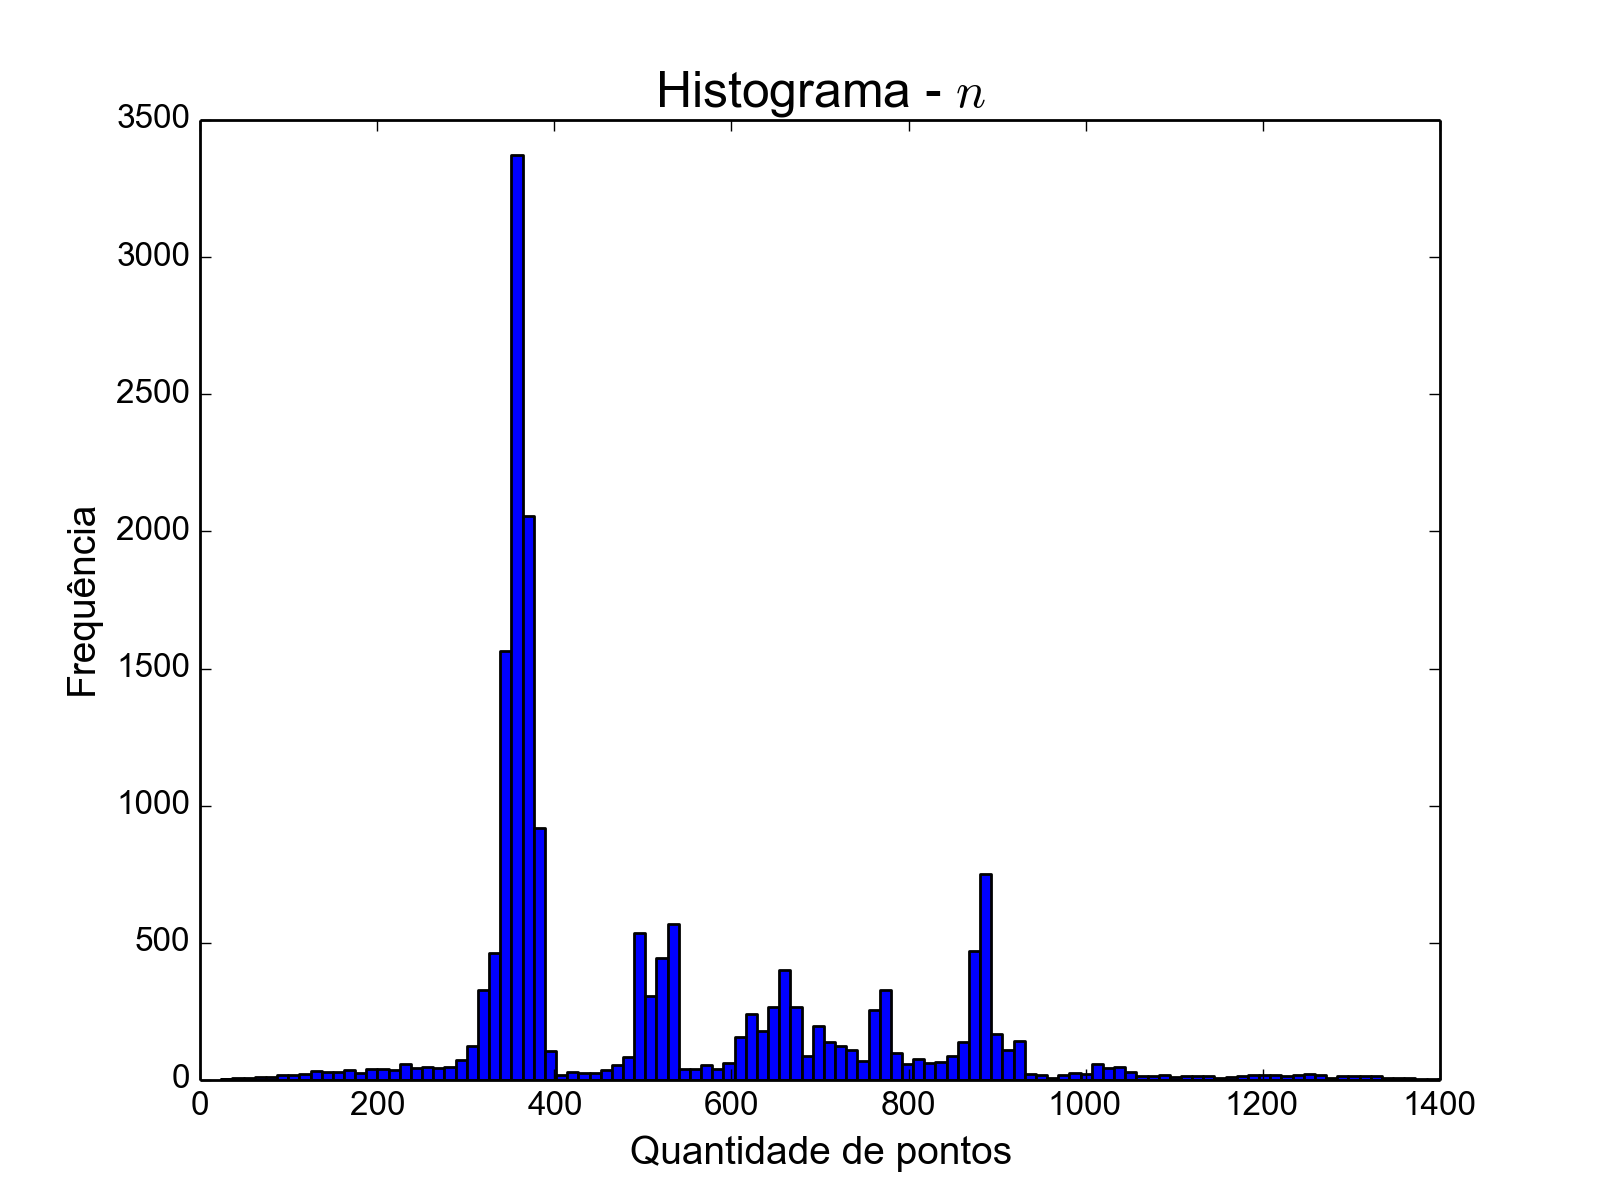
\includegraphics[width=0.6\linewidth]{hist_n.png}
  \caption[Histograma sobre quantidade de pontos.]{Histograma sobre a quantidade de pontos nos dados das RR Lyraes. A quantidade com maior frequência é $k = 352$.}
  \label{fig:histo_n}
\end{figure}

Tendo obtido a amostragem, podemos construir dados sintéticos variando a frequência de pontos e o nível de ruído para estudar como o método se comporta com esses sinais. O sinal sintético é construido pela expressão \ref{eq:dado_sint} em que os termos $A_i$ são dados por \citet{ce} e \citet{entropy} como sendo
$A_0 = 15$, $A_1 = -0.5$, $A_2 = 0.15$ e $A_3 = -0.05$ . O período utilizado para criar o sinal será $P = 0.576$ dias, pois de acordo com \citet{lyraes} esse é o valor de período médio das RR Lyraes do catálogo.

\begin{figure}[ht]
\centering
\begin{subfigure}{.5\textwidth}
  \centering
  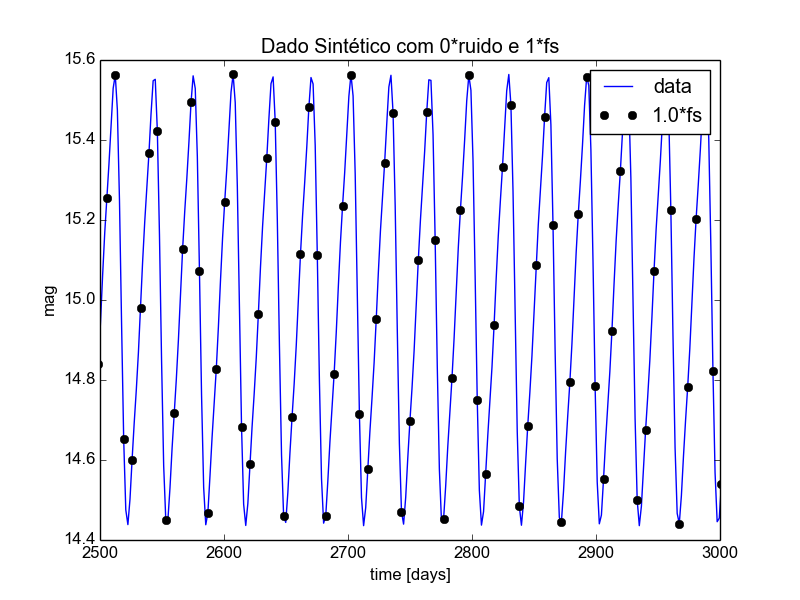
\includegraphics[width=\linewidth]{dado_sintetico_0_ruido_1_amos.png}
  \caption{Dado sem ruído e com amostragem padrão}
  \label{fig:1amos}
\end{subfigure}%
\begin{subfigure}{.5\textwidth}
  \centering
  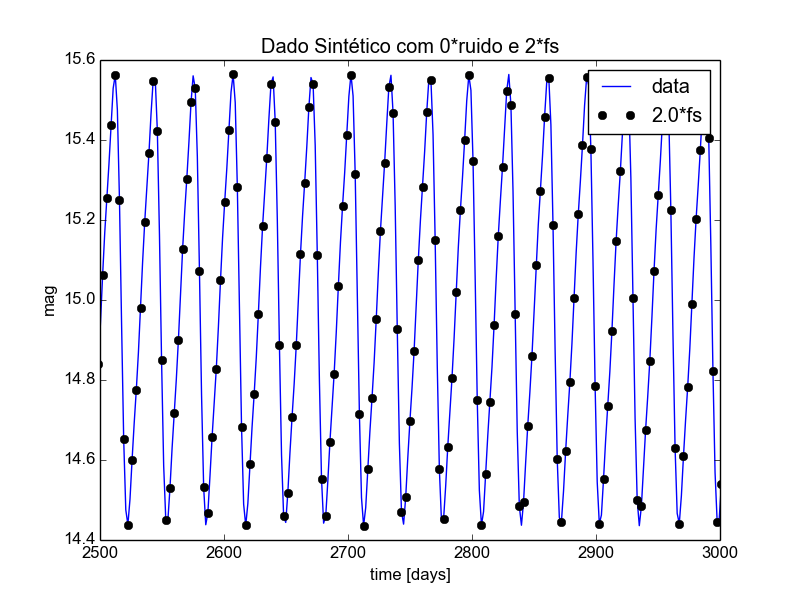
\includegraphics[width=\linewidth]{dado_sintetico_0_ruido_2_amos.png}
  \caption{Dado sem ruído e $k=2$}
  \label{fig:2amos}
  \end{subfigure}
\\
\begin{subfigure}{.5\textwidth}
  \centering
  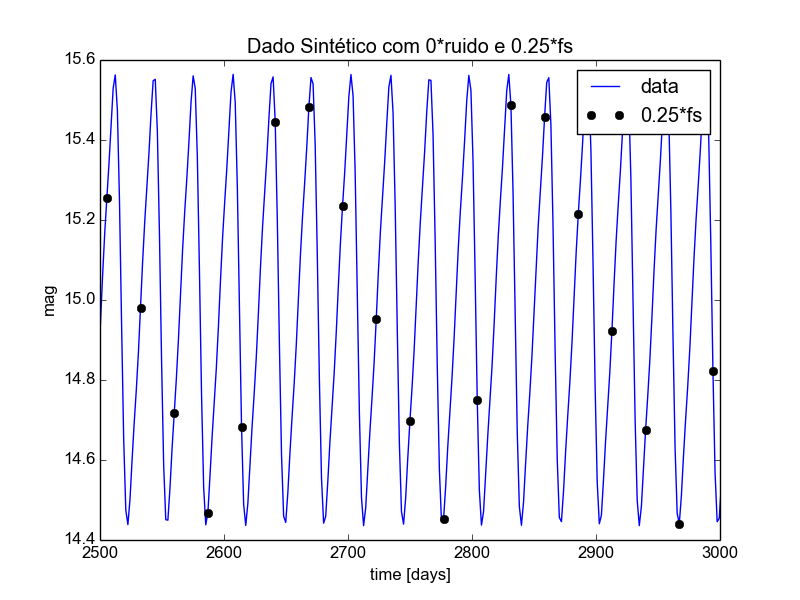
\includegraphics[width=\linewidth]{dado_sintetico_0_ruido_0_25_amos.png}
  \caption{Dado sem ruído e $k=1/4$}
  \label{fig:025amos}
\end{subfigure}%
\begin{subfigure}{.5\textwidth}
  \centering
  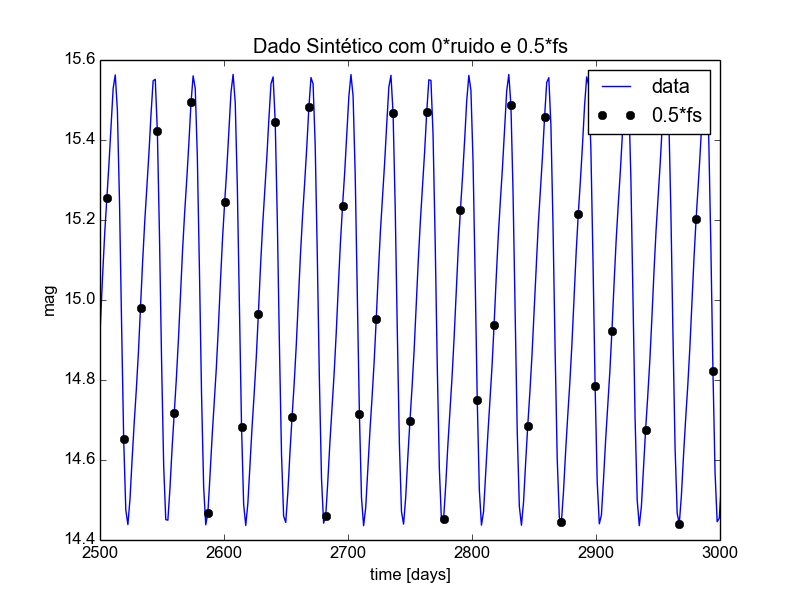
\includegraphics[width=\linewidth]{dado_sintetico_0_ruido_0_5_amos.png}
  \caption{Dado sem ruído e $k=1/2$}
  \label{fig:05amos}
  \end{subfigure}
\caption[Curva de luz sintética.]{Exemplos de curvas de luz sintética. Os exemplos foram criados sem ruído, $B=0$, e variando $k$. A linha azul representa o sinal original completo e os pontos e linha preta correspondem a observação com a amostragem $k$.}
\label{fig:exemplo_curva_luz}
\end{figure}


Para estudar a influência da amostragem nos dados, o vetor $t$ será criado utilizando os valores obtidos pelos histogramas de tempo inicial ($t_i = 2152,5019$) e final ($t_f = 4539,4593$) e a variação de pontos $dt$ será construído pela relação:
\begin{align}
dt = \frac{1}{f}
\end{align}
Em que $f = k \times f_s$, ou seja, a frequência de pontos $f$ será um parâmetro de escala $k$ vezes a amostragem $f_s$ dos dados. Desta forma, variando o parâmetro $k$ de $0,25$ a $4,0$ com um intervalo de $0,25$ e variando o parâmetro de escala para o ruído $B$ de $0,0$ até $1,0$ com intervalo de $0,05$, foram criadas 300 curvas de luz para serem analisadas. Quatro exemplos de curva de luz sintética gerada pelo método acima podem ser vistas na figura \ref{fig:exemplo_curva_luz}.




Na figura \ref{fig:exemplo_curva_luz}, os pontos e linha preta correspondem aos pontos de observação e a linha contínua azul seria o sinal original completo. Podemos perceber que quanto maior a amostragem, maior a quantidade de pontos.

\begin{figure}[H]
\centering
\hspace{-2.5cm}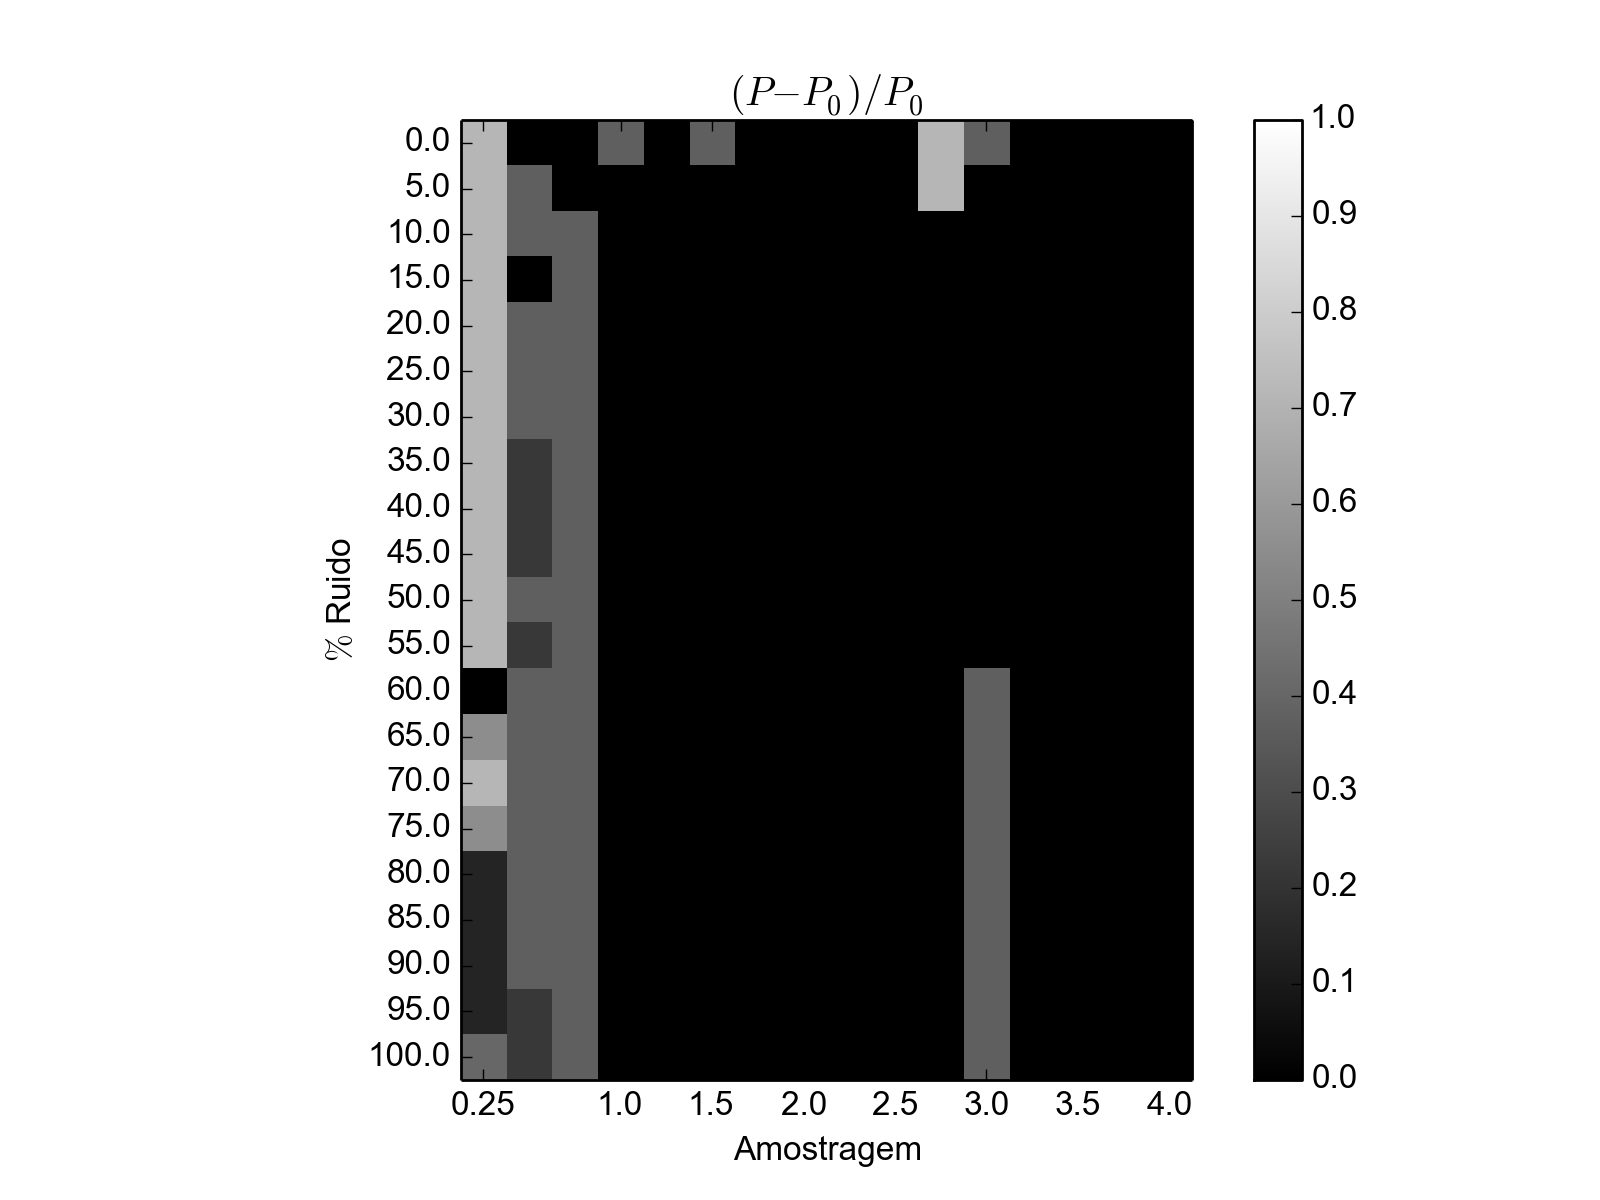
\includegraphics[scale=.8]{ce_inshow.png}
\caption[Resultados obtidos em escala de cinza.]{Resultados obtidos em escala de cinza. O eixo das abcissas representa o parâmetro de escala $k$ da amostragem e o eixo das ordenadas representa a variação do parâmetro de escala $B$ para o ruído. Quanto mais escura a cor do quadrado mais correto o valor calculado pela entropia de Shannon condicional.}
\label{fig:imshow}
\end{figure}

A figura \ref{fig:imshow} nos mostra um mapa de cor em escala de cinza entre parâmetro de escala $B$ do ruído e o parâmetro de escala $k$ da amostragem. A cor representa o valor $|(P - P_0)/P_0|$, ou seja, quanto o período calculado está variando em relação ao período original. A cor mais escura representa o valor 0 (período calculado = período real) e quanto mais clara a cor, maior o desvio do período.



%Obtendo a amostragem, podemos construir dados sintéticos variando a amostragem e o nível de ruído afim de estudar o comportamento do método. De acordo com \cite{ce} e \cite{entropy}, para construir dados sintéticos semelhantes com os dados observacionais da maioria dos Surveys de estrelas variáveis, podemos utilizar a seguinte expressão,
%\begin{align}
%m(t) &= A_0 + \sum_i^3 A_n \sin \Big( \frac{2 k \pi t}{P} \Big) + B \eta
%\end{align}
%em que $B$ é um fator de escala para o ruido entre \(0.0\) e \(1.0\), \(\eta\) é uma distribuição gaussiana com média zero e desvio unitário e \(P\) é o período médio das RRlyraes que, segundo \cite{lyraes} é de \(0.576\) dias.
%
%A influencia da amostragem está no vetor \(t\) que é construindo a fim de representar de forma mais fiel possível os dados do Catálogo OGLE-III. Sendo assim, o vetor tempo é construído com os seguinte parâmetros: tempo inicial de \(2152.5019\) HJD, tempo final de \(4539.4593\) HJD e espaçamento entre os pontos \(dt = 1 / f\) em que \(f = k \times f_s\) e \(k\) é um parâmetro de escala para a amostragem. Os tempos iniciais e finais foram escolhidos desta forma por serem os valores de maior frequência entre os dados das RRLyraes. Quatro exemplos de curva de luz sintética gerada pelo método acima podem ser vistas na figura \ref{fig:exemplo_curva_luz}.
%
%\begin{figure}[H]
%\centering
%\begin{subfigure}{.5\textwidth}
%  \centering
%  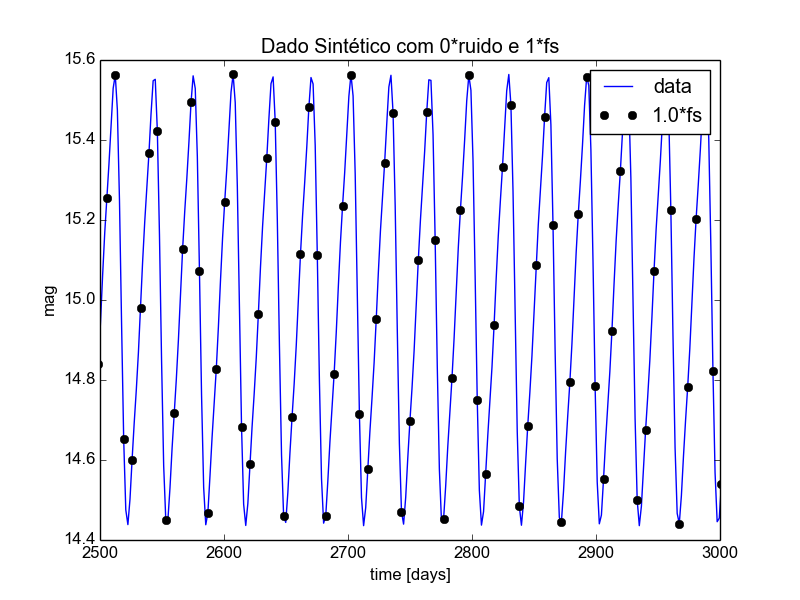
\includegraphics[width=\linewidth]{dado_sintetico_0_ruido_1_amos.png}
%  \caption{Dado sem ruído e com amostragem padrão}
%  \label{fig:1amos}
%\end{subfigure}%
%\begin{subfigure}{.5\textwidth}
%  \centering
%  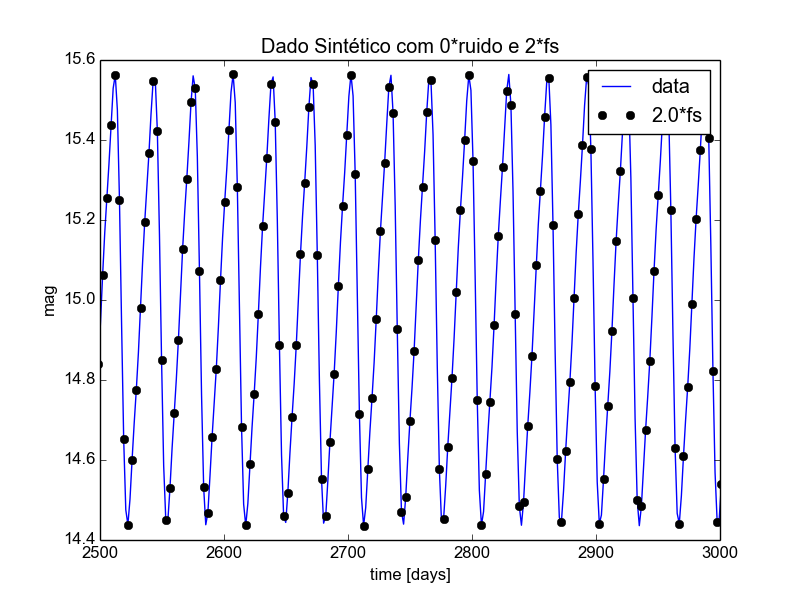
\includegraphics[width=\linewidth]{dado_sintetico_0_ruido_2_amos.png}
%  \caption{Dado sem ruído com $n=2$}
%  \label{fig:2amos}
%  \end{subfigure}
%\\
%\begin{subfigure}{.5\textwidth}
%  \centering
%  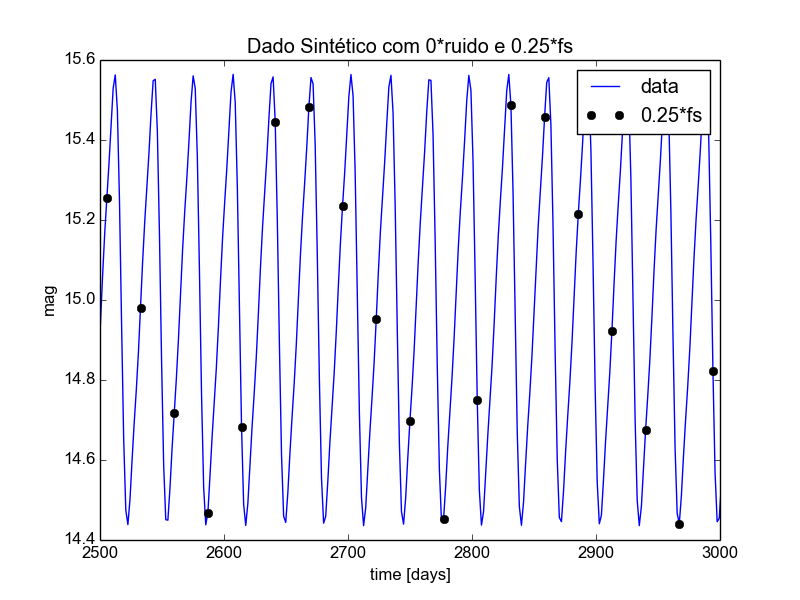
\includegraphics[width=\linewidth]{dado_sintetico_0_ruido_0_25_amos.png}
%  \caption{Dado sem ruído e com $n=1/4$}
%  \label{fig:025amos}
%\end{subfigure}%
%\begin{subfigure}{.5\textwidth}
%  \centering
%  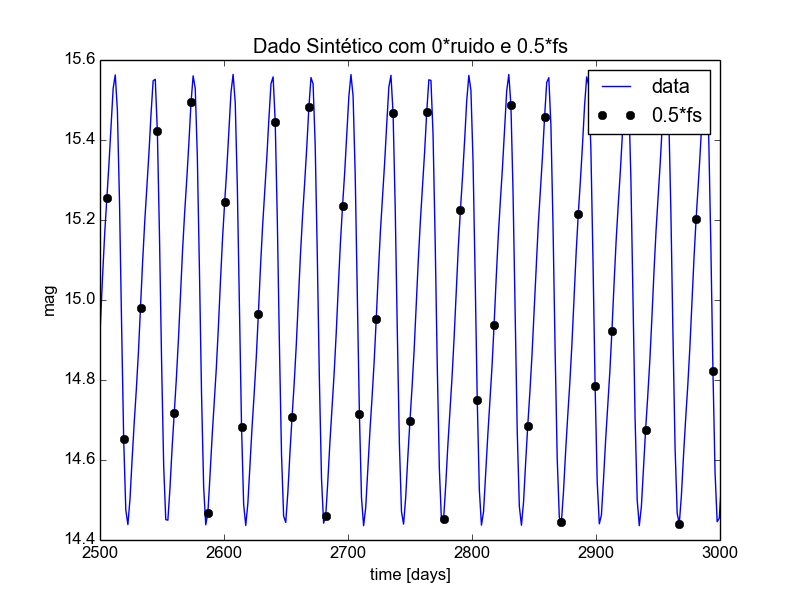
\includegraphics[width=\linewidth]{dado_sintetico_0_ruido_0_5_amos.png}
%  \caption{Dado sem ruído com $n=1/2$}
%  \label{fig:05amos}
%  \end{subfigure}
%\caption{Exemplos curva de luz sintética}
%\label{fig:exemplo_curva_luz}
%\end{figure}
%
%Na figura \ref{fig:exemplo_curva_luz}, os ponto pretos são os pontos de observação e a linha contínua é o dado original com \(n=1\). Podemos perceber que quanto maior a amostragem, maior a quantidade de pontos, assim o método aplicado a um dado com uma grande amostragem deve retornar um período com maior precisão do que comparado à um dado com pequena amostragem.

%Então, para estudar a influencia da amostragem nos dados foram gerados dados sintéticos variando o parâmetro $k$ da amostragem de $0.25$ a $4$ com intervalo de $0.25$ e variando o fator de escala $B$ de $0.0$ até $1.0$ com intervalo de $0.05$ assim obtendo $300$ curvas de luz. No momento, estamos pensando em como demonstrar os resultados obtidos. Uma forma para demonstrar os dados é fazendo um mapa de cor entre ruído e amostragem onde a cor representa o valor \(|(P - P_0)/P_0|\), ou seja, quanto que o período calculado está variando em relação ao período original. O mapa de cor é feito em escala de cinza, em que a cor mais escura representa o valor 0 (período calculado = período real) e quanto mais clara a cor, maior o desvio do período.	%o período calculado menos o período real do sinal dividido pelo período real, em  uma escala de cinza.



Podemos observar que a partir do parâmetro de escala $k=1,0$ para a amostragem, todos os resultado calculados foram corretos, não importando o nível de ruído, com exceção da faixa entre os ruídos $60\%$ e $100\%$ para $k=3$ que apresentam um resultado $\approx 0,4$. Essa exceção significa que o resultado obtido é aproximadamente a metade do período real.


%Os valores iguais a zero (cor preta) representam as configurações em que o método de entropia condicional calculou o período corretamente.

\section{Aplicação dos Resultados}

A grande importância da determinação de períodos de estrelas variáveis está na possibilidade de calcular distâncias a partir da Lei de Leavitt. Desta forma, utilizando a equação \ref{eq:leavitt_law} para magnitude médias, ou seja,
\begin{align}
\bar{M_i} = a \log P_i + b
\end{align}
e convertendo para a magnitude aparente média através da equação \ref{eq:dist_ext}, %para o módulo de distância,
\begin{align}
\bar{m_i} = a \log P_i + b + \mu_i + A_{\lambda_i} \label{eq:cap4_pl}
\end{align}
é possível calcular as constantes $a$ e $b$ utilizando o método dos mínimos quadrados para obter a relação entre o período e a luminosidade aparente. A correção para a extinção interestelar $A_\lambda$ é dada pelo mapa de \citet{Pejcha2009}.


Segundo \citet{Nikolaev2004}, o termo $\mu_i$ na equação \ref{eq:cap4_pl} pode ser escrito em duas partes:
\begin{align}
\mu_i = \bar{\mu} + \Delta \mu_i \label{eq:cap4_mod_dist}
\end{align}
Em que $\bar{\mu}$ é o modulo de distância médio para toda a Grande Nuvem de Magalhães e $\Delta \mu_i$ é a variação na distância para cada estrela. Portanto, podemos reescrever a equação \ref{eq:cap4_pl} como:
\begin{align}
\bar{m_i} = a \log P_i + b^\prime + \Delta \mu_i + A_{\lambda_i}
\end{align}
Em que o termo $\bar{\mu}$ foi incorporado na nova constante $b^\prime$.
Os resultados obtidos para essas constantes utilizando o método dos mínimos quadrados são apresentados na tabela \ref{tab:pl_relacao} para os 4 tipos de estrelas utilizados neste trabalho. As figuras \ref{fig:pl_cep} e \ref{fig:rr_pl} mostram a relação calculada sobre os dados.

\begin{table}[ht]
\begin{center}
\caption{Constantes da Relação PL.}
\begin{tabular}{c|c|c}
\toprule%\hline
Objeto & $a$ & $b^\prime$ \\
\midrule%\hline
Cefeida FU & $-1,292$ & $16,878$ \\
Cefeida FO & $-1,573$  & $16,558$ \\
RR Lyrae AB & $-0,721$ & $18,363$\\
RR Lyrae C & $-0,022$ & $18,841$\\
\bottomrule%\hline
\end{tabular} \\
\label{tab:pl_relacao}
\end{center}
\end{table}



Obtendo essas relações, é possível calcular a variação na distância $\Delta \mu_i$ de cada uma das estrelas pelo residual entre a Lei de Leavitt e a magnitude média obtida pelos dados do catálogo, ou seja,
\begin{align}
\Delta \mu_i = \bar{m}_{OGLE} - \bar{m_i}
\end{align}
e o modulo de distância real é obtida pela equação \ref{eq:cap4_mod_dist} considerando uma distância média de $50\si{kpc}$ ou $\bar{\mu} = 18,495$ \citep{Pejcha2009}. Tendo calculado o modulo de distância para todas as estrelas, a distância é obtida pela equação \ref{eq:dist_vela_padrao} em Parsec.


\begin{figure}[ht]
\centering
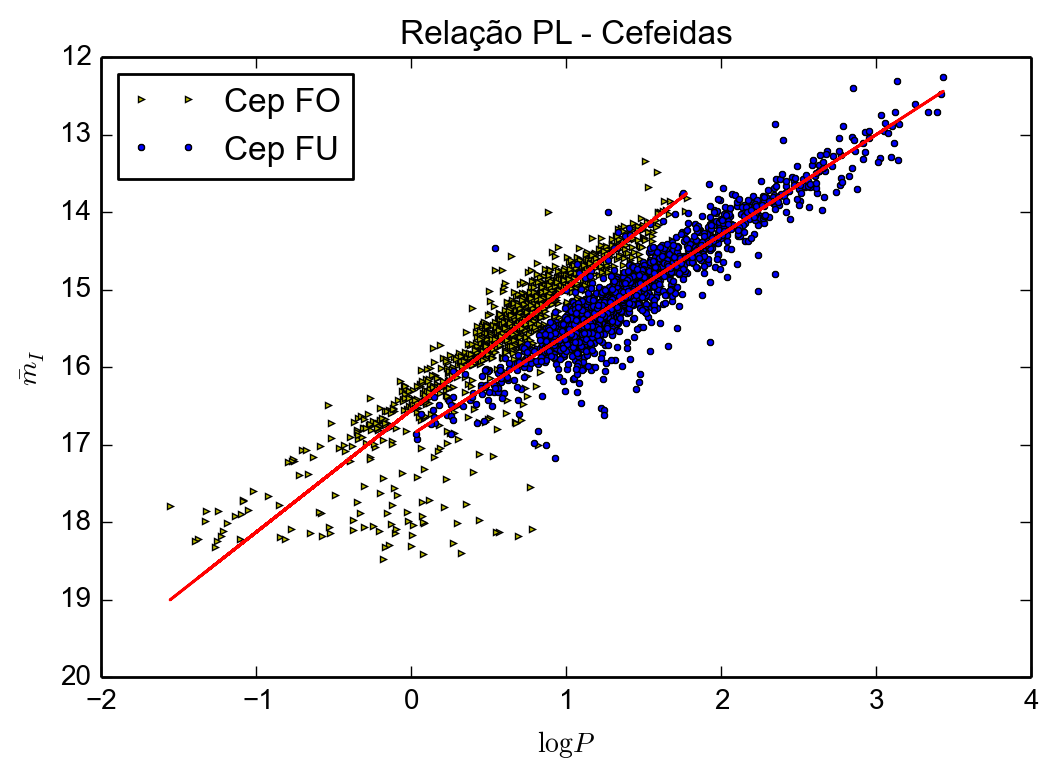
\includegraphics[width=0.6\linewidth]{cep_relacaoPL.png}
\caption[Relação PL para Cefeidas.]{Relação PL para as Cefeidas tipo FU e FO. O eixo das abcissas representa o logaritmo dos períodos calculados utilizando o método de entropia de Shannon condicional. O eixo das ordenadas representas a magnitude média de cada estrela na banda I obtidos no catálogo OGLE.}
\label{fig:pl_cep}
\end{figure}
%utilizando a equação \ref{eq:dist_ext} da seguinte forma: Sendo o modulo da distância dado pela relação,
%\begin{align}
%\mu = m - M - A_\lambda
%\end{align}
%e a magnitude absoluta obtida pela lei de Leavitt,
%\begin{align}
%M = a \log P + b
%\end{align}
%substituindo $M$ no modulo da distância,
%\begin{align}
%\mu = m - a \log P - b - A_\lambda
%\end{align}
\begin{figure}[!ht]
\centering
\begin{subfigure}{.5\textwidth}
  \centering
  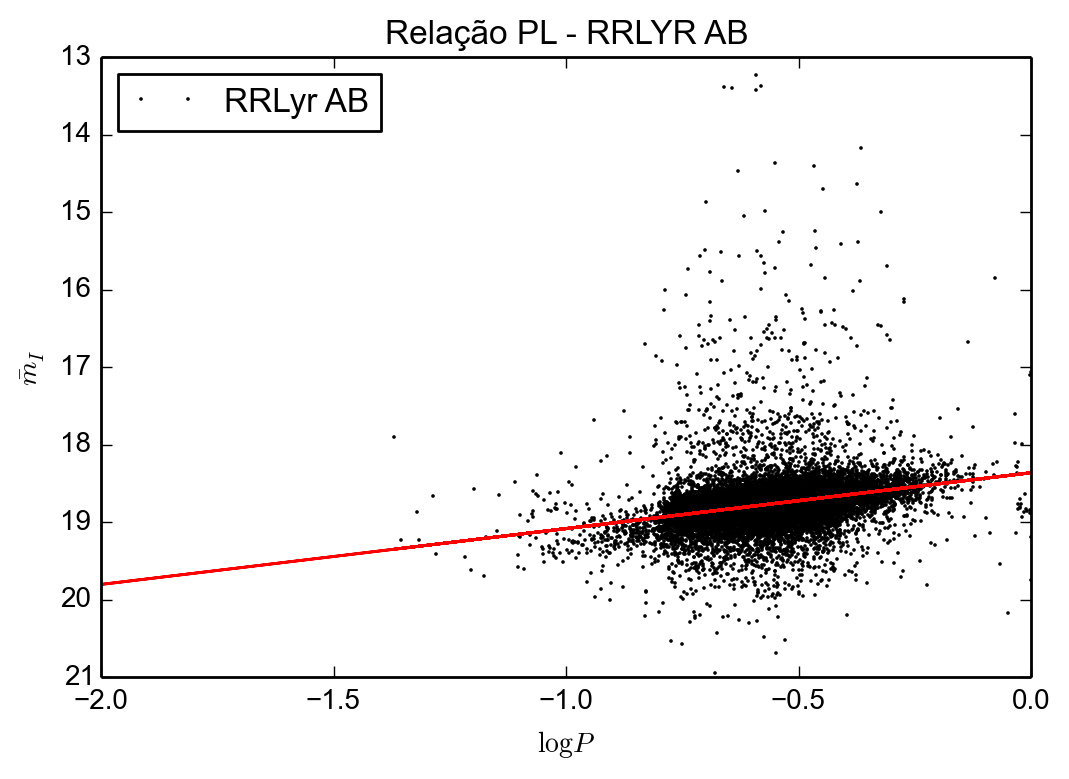
\includegraphics[width=\linewidth]{rrab_relacaoPL.png}
  \caption{RR Lyraes AB}
  \label{fig:ab_pl}
\end{subfigure}%
\begin{subfigure}{.5\textwidth}
  \centering
  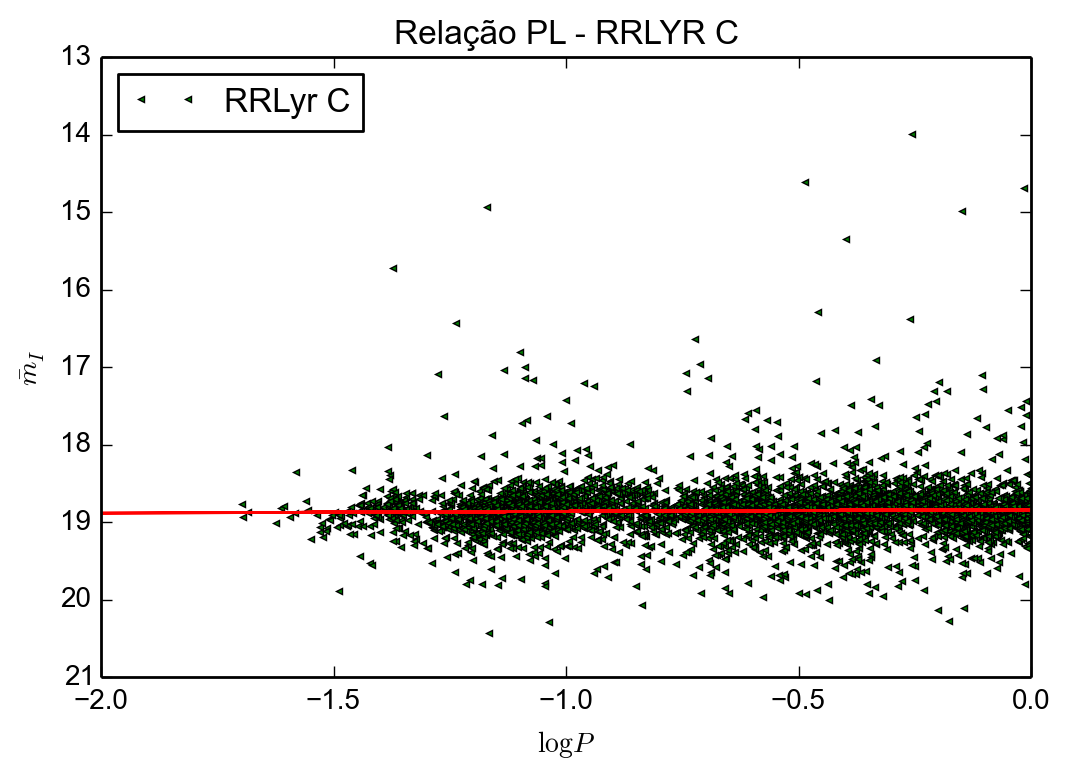
\includegraphics[width=\linewidth]{rrc_relacaoPL.png}
  \caption{RR Lyraes C}
  \label{fig:c_pl}
  \end{subfigure}
\caption[Relação PL para RR Lyraes.]{Relação PL para as estrelas RR Lyraes tipo AB (esquerda) e C (direita). O eixo das abcissas representa o logaritmo dos períodos calculados utilizando o método de entropia de Shannon condicional. O eixo das ordenadas representas a magnitude média de cada estrela na banda I obtidos no catálogo OGLE.}
\label{fig:rr_pl}
\end{figure}
%e isolando a magnitude
%\begin{align}
%m  = a \log P + b + A_\lambda + \mu
%\end{align}
%\textcolor{red}{continuar...}

Para determinar a estrutura da Grande Nuvem de Magalhães é necessário calcular a distribuição em coordenadas cartesianas a partir dos dados de ascensão reta ($\alpha$) e declinação ($\delta$) obtidos do catálogo OGLE e dos dados de distância ($r$) calculados anteriormente. Desta forma, será feita a transformação de um espaço de coordenadas ($\alpha$, $\delta$, $r$) para as coordenadas ($x$, $y$, $z$) considerando que a Grande Nuvem de Magalhães é centrada nas posições ($\alpha_0$, $\delta_0$, $r_0$). As transformações de coordenadas são dadas por \citet{Deb2014} e mostradas a seguir:
\begin{align}
x &= -r \sin \left(\alpha - \alpha_0 \right) \cos \left( \delta \right) \notag \\
y &= r \sin \left( \delta \right) \cos \left( \delta_0 \right) - r \sin \left( \delta_0 \right) \cos \left( \alpha - \alpha_0 \right) \cos \left( \delta \right) \label{eq:cap4_trans}\\
z &= r_0 - r \sin \left( \delta \right) \sin \left(\delta_0 \right) - r \cos \left( \delta_0 \right) \cos \left( \alpha \right) - \alpha_0 \cos \left( \delta \right) \notag
\end{align}

%\begin{align}
%x = -D \sin (\alpha - \alpha_0) \cos(\delta) \\
%y = D \sin (\delta) \cos (\delta_0) − D \sin (\delta_0) \cos (\alpha - \alpha_0) \cos( \delta) \\
%z = D_0 - D \sin(\delta)\sin(\delta_0) - D \cos (\delta_0) \cos( \alpha ) - \alpha_0 \cos (\delta)
%\end{align}

O centro da Grande Nuvem de Magalhães é obtido a partir dos valores médios das coordenadas equatoriais $\alpha$ e $\delta$ e possui valores $\alpha_0 = 80,240^\circ$ e $\delta_0 = -69.608^\circ$, como mostrado na figura \ref{fig:equatorial}.

\begin{figure}[!ht]
\centering
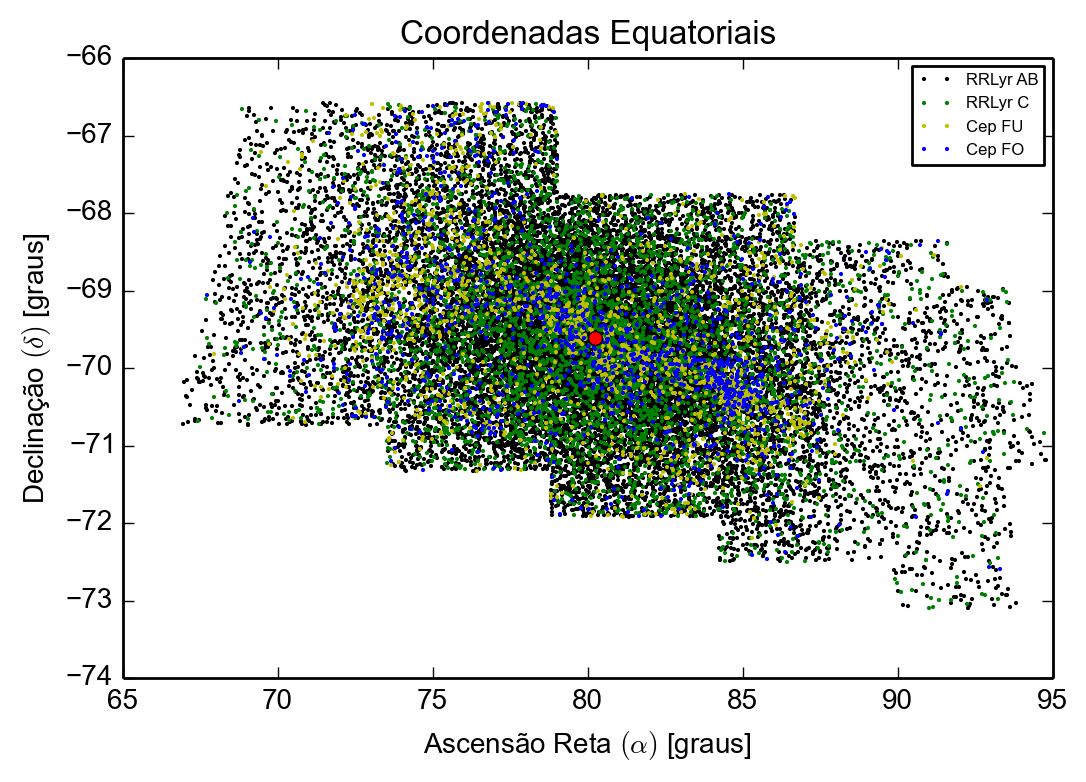
\includegraphics[width=0.6\linewidth]{equatorial.png}
\caption[Distruibuição de estrelas em coordenadas equatoriais.]{Distribuição das posições das estrelas do pulsantes do catálogo OGLE em coordenadas equatoriais. O ponto vermelho no centro representa a centroide e possui posição $\alpha_0 = 80,240^\circ$ e $\delta_0 = -69,608^\circ$.}
\label{fig:equatorial}
\end{figure}

Assim, utilizando as transformações \ref{eq:cap4_trans} foi calculado a distribuição tridimensional da Grande Nuvem de Magalhães como mostra a figura \ref{fig:plot3d}.

\begin{figure}[!ht]
\centering
\begin{subfigure}{.5\textwidth}
\centering
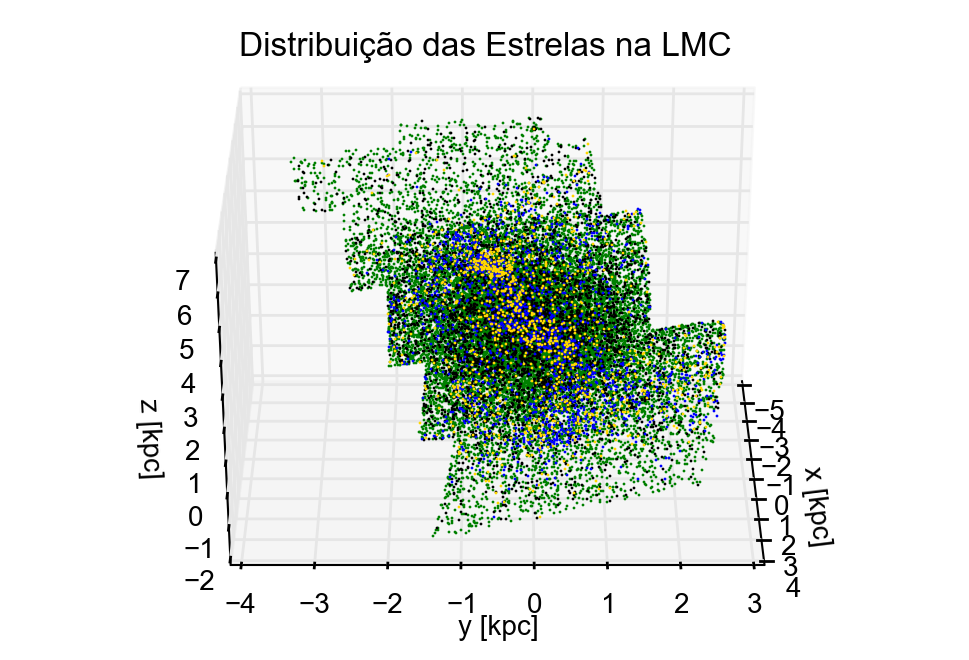
\includegraphics[width=\linewidth]{3d_plot_0.png}
\caption{0}
\end{subfigure}%
\begin{subfigure}{.5\textwidth}
\centering
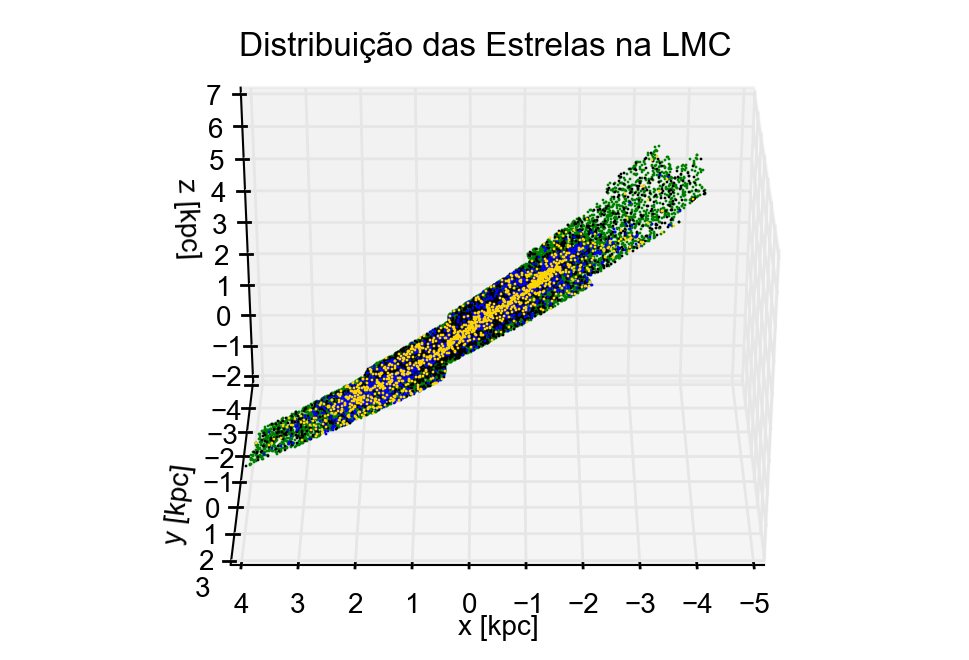
\includegraphics[width=\linewidth]{3d_plot_90.png}
\caption{90}
\end{subfigure}
\\
\begin{subfigure}{.5\textwidth}
\centering
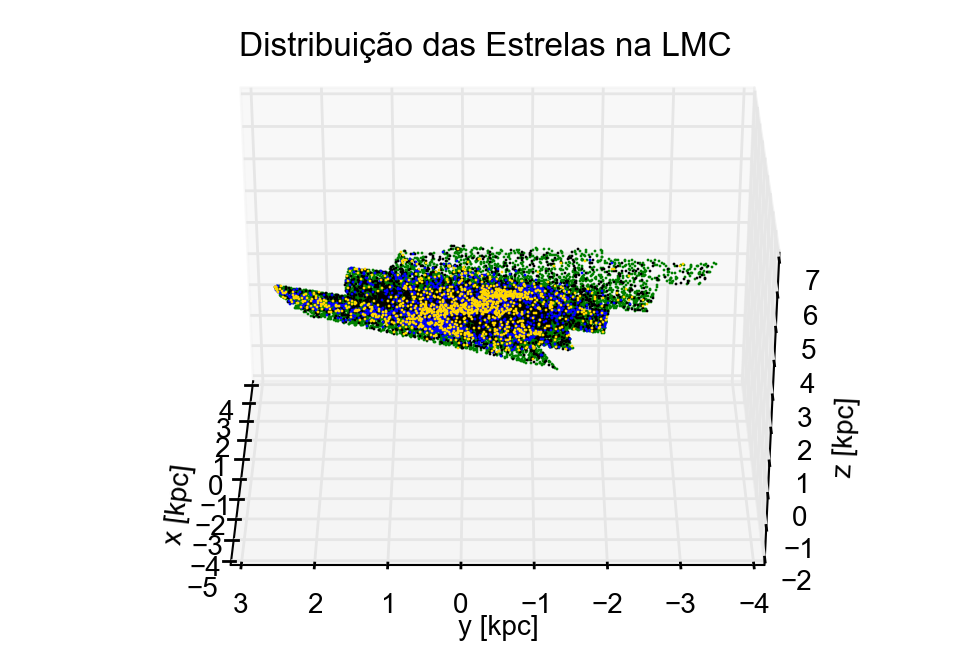
\includegraphics[width=\linewidth]{3d_plot_180.png}
\caption{180}
\end{subfigure}%
\begin{subfigure}{.5\textwidth}
\centering
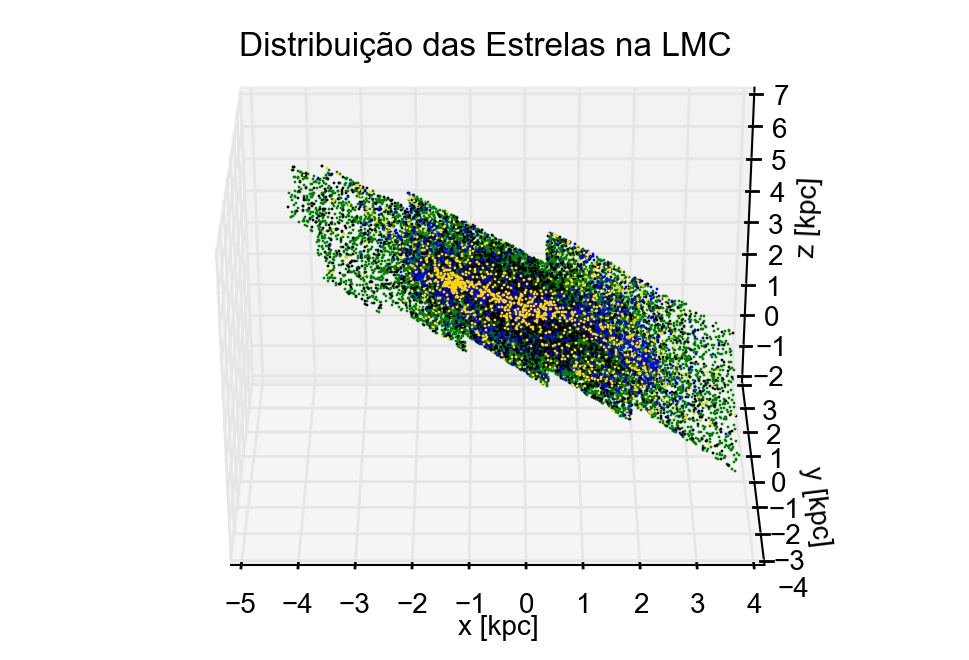
\includegraphics[width=\linewidth]{3d_plot_270.png}
\caption{270}
\end{subfigure}
%\includegraphics[width=0.8\linewidth]{plot3d.png}
\caption[Distruição 3D da Grande Nuvem de Magalhães.]{Distruição tridimensional da Grande Nuvem de Magalhães em coordenadas cartesianas. São mostradas a distruição em 4 ângulos de visão, $0^\circ$ (A), $90^\circ$ (B), $1800^\circ$ (C), $270^\circ$ (D) }
\label{fig:plot3d}
\end{figure}

Assim é possível perceber como a galaxia se distribui espacialmente e perceber que a maioria das estrelas se concentram na região central.

%\section{Conclusão}

%A observação e detecção de períodos de estrelas variáveis é fundamental para descrição desses objetos astronômicos e para a determinação de distâncias. Embora existam diversos métodos para o calculo de período, o desenvolvimento de técnicas que sejam confiáveis e possam ser aplicadas para dados com espaçamento variável entre os pontos de observação é de grande importância em uma realidade em que há dificuldades para observação dos telescópios, sendo essas dificuldades devido ao tempo disponível de observação e as condições climáticas. O método apresentado neste trabalho, a entropia de Shannon condicional, é uma técnica simples de ser entendida e aplicada, possuindo  um embasamento matemático dentro da teoria da informação, o que faz com que a sua análise estatística seja conhecida, fato que não é verdade para alguns métodos de detecção de períodos. Além disso, o método  apresenta um desempenho mais do que satisfatório com uma taxa de acerto maior do que $97\%$ para as $25707$ estrelas pulsantes do catálogo OGLE-III. Além disso, a análise dos dados sintéticos afirma que o método é confiável para qualquer nível de ruído desde que a frequência de pontos dos dados seja maior do que $f_s = 0,1473$. Por fim, com a figura \ref{fig:imshow} foi possível  construir uma ferramenta que nos indica como os dados influenciam no resultado do método, ou ainda, partindo do resultado que se espera obter, é possível determinar como a observação nos telescópios devem ser conduzidas. Parte dos resultados obtidos nesse trabalho foram apresentados em \citet{gabe1} e \citet{gabe2}.

%\input{Chapters/Chapter2} 
%\input{Chapters/Chapter3}
%\input{Chapters/Chapter4} 
%\input{Chapters/Chapter5} 

%----------------------------------------------------------------------------------------
%	THESIS CONTENT - APPENDICES
%----------------------------------------------------------------------------------------

\appendix % Cue to tell LaTeX that the following "chapters" are Appendices

% Include the appendices of the thesis as separate files from the Appendices folder
% Uncomment the lines as you write the Appendices

%\input{Appendices/AppendixA}
%\input{Appendices/AppendixB}
%\input{Appendices/AppendixC}

%----------------------------------------------------------------------------------------
%	BIBLIOGRAPHY
%----------------------------------------------------------------------------------------

\printbibliography[heading=bibintoc]

%----------------------------------------------------------------------------------------

\end{document}